\documentclass{statsmsc}

% Vim note: zo, zc and zm to open and close folds, and close all folds

% Commands {{{

% TODO: alternative title "Automated (data) preprocessing for deep sequence models"
%                  or     "Automated (data) preprocessing for deep neural networks"
\title{Automated data preprocessing for deep neural networks}
\author{Marcus Alexander Karmi September}
\CID{01725740}
\supervisor{Francesco Sanna Passino (Imperial College London), \newline Leonie Tabea Goldmann, and Anton Hinel (American Express)}
\date{\today}
\logoimg{}


% THIS IS WHERE NEW COMMANDS CAN BE DEFINED
% commands below only used in the proof; otherwise can be deleted
\newcommand{\consta}{a}
\newcommand{\X}{X}
\newcommand{\EE}[1]{ \mathrm{E} [ #1 ] }
\newcommand{\inparenth}[1]{\left( #1 \right)}

% }}}

\begin{document}

%%%%% Heading, Abstract and Acknowledgements %%%%%
% Heading {{{

% Generates the Title Page
\maketitle


% Generates plagiarism declaration
\declarationname{Marcus Alexander Karmi September}
\declarationdate{\today}
\declaration

\begin{abstract}
    This project proposes and compares different approaches to data preprocessing for
    increasing the predictive performance of deep neural networks.
    Data preprocessing is an important part of any machine learning modelling task, and
    can have a significant impact on both performance and training efficiency, especially
    if the dataset contains irregularities such as skewness, outliers, or multiple modes.
    All these characteristics are common in real-world datasets, yet a lot of papers only consider
    simple and traditional preprocessing methods such as min-max normalization and standard scaling, which might
    not properly handle these irregularities. 
    In this thesis, three novel more sophisticated preprocessing methods are proposed.
    Instead of using a fixed normalization scheme like traditional methods do, the
    proposed methods adapts the normalization to the given task, giving significant
    performance improvements. These methods are applied
    and evaluated on three datasets: a synthetic dataset, a credit default prediction
    time-series dataset provided by American Express, and a real-world financial forecasting dataset.
    The methods are also compared to related work on time-series preprocessing by \cite{dain} and \cite{bin}.
    Our results demonstrate better performance of the proposed preprocessing methods on all three
    datasets considered.



\end{abstract}

\begin{acknowledgements}
    First and foremost, I want to thank my supervisors Francesco Sanna Passino,
    Leonie Tabea Goldmann, and Anton Hinel for the continued guidance and help they
    have provided me throughout the project. Their advice and ideas have been very
    helpful.
    I also want to thank Andy Thomas and the Department of Mathematics for providing me with
    access to a powerful GPU system that proved very useful during my computational experiments.
    Lastly, I want to thank my parents Alexander and Sarah, and my sister Olivia,
    for their unconditional love and encouragement.

    \begin{flushright}
        \textit{-Marcus}
    \end{flushright}

\end{acknowledgements}

{\thispagestyle{plain}
    \tableofcontents
}
% }}}

%%%% Notation %%%%
% Notation {{{
{\chapter*{Notation}\thispagestyle{plain}
    $\bfx, \bfy, \bfz\in\R^d$ are $d$-dimensional vectors, and unless otherwise specified, they are
    treated as column vectors

    $\bfX \in \R^{p \times q}$ is a matrix

    $\bfX^{(i)} \in \R^{d \times T}$ denotes the $i$th time-series in a dataset, corresponding to a multivariate time-series of length $T$ and dimensionality $d$

    $\bfx^{(i)}_t \in \R^d$ denotes the $d$-dimensional feature vector at timestep $t$ in the $i$th time-series in the dataset

    $\bfx^{(i)}_{*,k} \in \R^T$ denotes the $T$-dimensional slice of the $i$th time-series, only including the $k$th feature at each timestep

    $x^{(i)}_{t,j}\in\R$ is the $j$th feature at timestep $t$ in the $i$th time-series in the dataset

    $f(x)$ denotes a scalar function $f: \R \rightarrow {\R}$ that maps a single element to a single element

    $\mathbf{f}(\bfx)$ denotes a vector function $\mathbf{f}:\R^d \rightarrow {\R^d}$ applied to a $d$-dimensional vector

    $\oplus, \ominus, \odot$, and $\oslash$ denotes addition, subtraction, multiplication, and division, respectively, applied element-wise between two $d$-dimensional vectors. For example, $\bfx \oslash \bfy$ denotes the vector where each element of $\bfx$ has been divided by the corresponding element of $\bfy$

    $\mathcal{D}$ denotes a dataset

    $\mathcal{B}$ denotes a set of indices from a dataset, referred to as a \textit{batch}

    $\mathbf{J}_{\bfZ \rightarrow {\bfY}}$ and $\mathbf{J}_{\mathbf{f}}$ both denote the Jacobian matrix of a function $\mathbf{f} : \R^d \rightarrow {\R^d}$ that maps samples $\bfz \sim \bfZ$ to samples $\bfy \sim \bfY$, that is,
    $\bfy=\mathbf{f}(\bfz)$

    $\mathbb{I}(p)$ denotes the indicator function and takes value 1 when condition $p$ is true,
    0 otherwise.

    $\#A$ and $|A|$ both refer to the cardinality of a set $A$, that is, the number of elements contained in $A$

    $\mathcal{N(\cdot,\cdot)}$ denotes a normal, also known as Gaussian,
    distribution. For example, $X \sim \mathcal{N}(\mu=0, \sigma=5)$ means $X$
    is a random normal variable with mean 0 and variance 25

    $f \circ g$ denotes function composition. For example if $h=f \circ g$, then $h(x)=f(g(x))$

% }}}

%%%% Abbreviations and acronyms %%%%
% Abbreviations {{{
{\chapter*{Abbreviations}\thispagestyle{plain}
    \begin{acronym}[TDMA]
        \acro{DAIN}{Deep Adaptive Input Normalization}
        \acro{RDAIN}{Robust Deep Adaptive Input Normalization}
        \acro{EDAIN}{Extended Deep Adaptive Input Normalization}
        \acro{EDAIN-KL}{Extended Deep Adaptive Input Normalization, optimised with Kullback–Leibler divergence}
        \acro{BIN}{Bilinear Input Normalization}
        \acro{pdf}[PDF]{probability density function}
        \acro{CDF}{cumulative density function}
        \acro{KL-divergence}{Kullbeck-Leibler divergence}
        \acro{PREPMIX-CAPS}{Preprocessing Mixture, optimised with Clustering and Parallel Search}
        \acro{API}{Application Programming Interface}
        \acro{GPU}{Graphics Processing Unit}
        \acro{RNN}{Recurrent Neural Network}
        \acro{GRU}{Gated Recurrent Unit}
        \acro{LSTM}{Long Short-Term Memory}
        \acro{ReLU}{Rectified Linear Unit}
        \acro{LOB}{limit order book}
        \acro{OLS}{ordinary least squares}
        \acro{PCA}{principal component analysis}
        \acro{RV}{Random variable}
        \acro{EDA}{Exploratory data analysis}
    \end{acronym}
}

% VERY IMPORTANT
% This command switches from Roman to Arabic numbering for main part of thesis
\mainmatter

% }}}

%%%%%%%%%%%%%%%%%%%%%%%%%%%%%%%%%%%%%%%%%%%%%%%%%%%%%%
\chapter{Introduction} %%%%     Introduction      %%%%
%%%%%%%%%%%%%%%%%%%%%%%%%%%%%%%%%%%%%%%%%%%%%%%%%%%%%%
% Introduction {{{

% TODO: in addition to methods as part of **MAIN CONTRIBUTIONS**, also present that additional
%       contribution is some novel insight on local- vs. global-ware normalization.

% Main content:


% Tips for writing the introduction:
% * Make it very clear what the **message** of the project is
% * Make the **research question** very clear
% * All statements made in introduction should have a good amount of
%   citations/papers to back it up. Looks very bad if making bold statements in
%   introduction without a paper backing it up!

% <<<<<<<<<<<<<<<<<<< Intro starts >>>>>>>>>>>>>>>>

% First paragraph: Narrowing in on research question/objective
% * 4-5 lines on general setup, with description of machine learning pipeline
% * "One often overlooked part is the preprocessing step \citep{....}", and not
%   many research papers on it
% * Yet this can have a significant impact on the performance \citep{....}
% * As such **present <research question>**
% * (Also including **motivating example from Amex dataset**, e.g. mention
%    skewed distributions, outliers, etc.)
% Note: the literature references in this paragraph focuses on honing in on
% preprocessing in machine learning in general, while the third paragraph picks
% up on this thread, and goes from preprocessing in ML to sophisticated
% preprocessing in deep learning for time-series data

% Explain pipeline

% Old start:
% Deep neural networks have contributed to remarkable progress
% for artificial intelligence, and have been applied in a wide
% variety of fields with great success \citep{dnn_survey}.
% New start:
Deep neural networks are able to learn highly complicated
relationships between input data and target labels, and have been successfully
applied to many difficult classification and prediction problems in a wide
variety of fields \citep{dnn_survey}.
There are many steps required when applying deep neural networks--%
or more generally, any machine learning model--to a problem. First, 
the data needs to be gathered, cleaned, and formatted into numerical,
machine-readable values. Then, these numerical values need to be
\textit{preprocessed} to facilitate model learning.
After this, features are designed from the processed data.
The model architecture, its hyperparameters, or both, then needs to be
chosen appropriately. This is followed by model optimisation and
evaluation using suitable metrics. These steps may then be reiterated
several times.

% Present some research
One step that is often overlooked or not given enough attention is the
\textit{preprocessing step} \citep{stanislav}. Yet, applying appropriate
preprocessing to the data can have significant impact on both performance and
training efficiency \citep{preprocess_origin,nawi,singh,dain,bin,mixture_ct}.
However, determining the most suitable preprocessing method can be time-consuming,
as such, the main purpose of this thesis is: \textit{\textbf{optimising the
predictive performance of neural networks through automated data preprocessing}}.  In
particular, we focus on preprocessing \textit{multivariate time-series} data for use
in \acp{RNN}, which is a neural network architecture designed for sequence data.
We intend to apply our discoveries to the credit default prediction dataset
provided by American Express, which
contains missing values, variables with skewed distributions and outliers. These are all
common characteristics in real-world datasets \citep{nawi,brits}.

% Second paragraph
% * Present strategy for approach the research question, which also ties in with structure of
%   the thesis?
% * Highlight the contributions of the project
To approach the research problem in question, we studied existing preprocessing methods
from the literature. We found that many of these were too simple and thus unable to handle
the many irregularities observed in our datasets. Therefore, more sophisticated adaptive
preprocessing methods were considered, and three new methods were proposed:
\textit{\acl{EDAIN}} (\acs{EDAIN}), \textit{\acl{EDAIN-KL}} (\acs{EDAIN-KL}),
and \textit{\acl{PREPMIX-CAPS}} (\acs{PREPMIX-CAPS}).
These were evaluated on a synthetic time-series dataset, generated with a
novel and flexible data generation procedure that we propose.
They were also evaluated on the credit default prediction dataset provided by American
Express and on a financial forecasting dataset. These two real-world datasets have
very different characteristics, which highlights the preprocessing methods' effectiveness and
limitations in different scenarios. 
On all three datasets, the proposed methods were compared to conventional preprocessing methods and 
to recent work on time-series preprocessing by \cite{dain} and \cite{bin}. In particular,
the proposed \acs{EDAIN} preprocessing method demonstrates
better performance on all three datasets considered.

% Third paragraph:
% Bit of an overview of the existing literature, narrowing in on time-series, DNNs, adaptive etc.
% * Many works study time-series(?) data preprocessing is a widely-studied area of
%   machine learning research, in deep learning? (insert many citations)
% * However, most of these methods are relatively simple static transformations,
%   therefore unable to handle the many irregularities commonly observed in real-world
%   datasets, such as multiple modes, skewness and outliers (cite dain, rdain, nawi)
% * There are more sophisticated adaptive preprocessing layers widely studied, but most of
%   these focus on preprocessing activations within the neural network (cite
%   batchnorm, improving batchnorm, etc.)
% * To the best of my knowledge, only \cite{dain,rdain} and \cite{bin} have looked at more
%   sophisticated methods for preprocessing time-series data before it enters the neural network
% * However, all of these methods have primarily been designed for financial time-series forecasting,
%   not general time-series data, which is the focus of this thesis.

Many works in the literature study how preprocessing methods can improve the predictive performance
of machine learning models in various fields
\citep{preprocess_origin,nawi,singh,dain,bin,mixture_ct}. However, most of these works
\citep{preprocess_origin,nawi,singh,mixture_ct} only consider traditional static transformations
and would therefore not be appropriate for handling the many irregularities and temporal
aspect present in the  time-series datasets considered in this thesis and certain other
real-world scenarios \citep{nawi,dain,rdain,bin}.
There are many sophisticated adaptive preprocessing methods
for normalizing data in neural network models \citep{huang2020,yu2022,batchnorm}, but most
of these focus on normalizing the activations within the neural network.
To the best of my knowledge, only \cite{dain,rdain,bin} have looked at more sophisticated
methods for preprocessing time-series data prior to it entering the neural network.
However, these works primarily focus on normalizing financial time-series for
forecasting tasks. As such, this thesis will shed some light on how more sophisticated
preprocessing methods can best be applied to time-series data in a general setting.

% Fourth paragraph: structure of the thesis
The remainder of the thesis is structured as follows. \Cref{ch:Background}
provides an overview of the deep learning models and techniques that were used
throughout the thesis, including a description of \acp{RNN}.
Additionally, an overview of existing preprocessing
methods from the literature are presented in this chapter. In
\cref{ch:Methods}, we present the main contributions of the thesis: Three novel
preprocessing methods named \acs{EDAIN}, \acs{EDAIN-KL}, and \acs{PREPMIX-CAPS}.
Then, in \cref{ch:Results}, the performance of the
proposed preprocessing methods are assessed and compared to existing work by
evaluating them on three different datasets: a synthetic dataset, the default
prediction dataset provided by American Express, and a financial forecasting
dataset. We then discuss the experimental results and highlight the different
preprocessing methods' advantages and limitations in \cref{ch:Discussion}.  In
\cref{ch:Conclusion}, we end the thesis with a conclusion and plans for future
work.
% Link to code
We note that an open-source implementation of all the preprocessing methods proposed,
along with scripts
to reproduce the experiments conducted in the thesis, can be found at
\url{https://github.com/marcusGH/automated-preprocessing-for-deep-neural-networks}, with
more implementation details in \cref{cha:imp_notes}.

% }}}

%%%%%%%%%%%%%%%%%%%%%%%%%%%%%%%%%%%%%%%%%%%%%%%%%%%%%%
\chapter{Background} %%%%        Background       %%%%
%%%%%%%%%%%%%%%%%%%%%%%%%%%%%%%%%%%%%%%%%%%%%%%%%%%%%%
\label{ch:Background}

% Introduction
% Introduction {{{

In this project, we make extensive use of deep learning methods, especially sequence models, as
both of the real-world datasets and the synthetic dataset we will be working with all contain
multivariate time-series.  Therefore, we start this chapter off with a background on deep
learning, building up to deep sequence models such as \acp{RNN}.
Another big part of the project is investigating the effect of different
preprocessing techniques applied to the data before it is passed to the deep neural network.
As such, this chapter also covers the most commonly used \textit{static preprocessing methods} used
in the literature. Additionally, we will look at the current state of the art when it comes
to preprocessing multivariate time-series data, which includes three
\textit{adaptive preprocessing methods} whose unknown parameters are trained in the same
fashion as neural networks.

% }}}

\section{Deep learning}% Deep learning
% Methods: Deep learning {{{
\label{sec:Deep learning}

% TODO: change wording somewhere to highlight that the multi-layer perceptron (MLP) model
%       is in fact non-linear by having non-linear activation functions between the layers.
%       Nvm, MLP is misnomer, so better to refer to it as feed-forward neural network

Deep learning has played a significant role in improving predictive performance in many fields,
ranging from financial forecasting \citep{dain,rdain,bin} to machine
translation \citep{gru_cho,attention} to computed tomography analysis
\citep{mixture_ct}. In this section, we provide a brief overview of how neural networks work and
how they are trained using a dataset. We do this by first describing the standard \textit{linear},
or feedforward-type, neural network. Then we move onto describing how neural networks are trained,
including descriptions of loss functions, stochastic gradient descent, and backpropagation. We will
also cover extensions to the standard training framework, including early stoppers, learning
rate schedulers and optimizers with adaptive learning rates.

\subsection{The standard linear neural network}%
\label{sub:The standard linear neural network}

The standard neural network consists of $L$ \textit{linear} layers, each containing
$n_1,n_2,\dots,n_L$ perceptrons, or \textit{units} \citep{dnn}. An input sample $\bfx \in \R^d$ can be fed
through the neural network, producing \textit{post-activations} at each layer, denoted
$\bfz^{(1)}, \dots, \bfz^{(L)}$. The post-activations are produced through weighted
connections between each neuron and all the neurons in the previous layer. If we let
$\bfz^{(0)}=\bfx \in \R^d$ denote the input and let $n_0=d$, we have for $\ell=1,\dots,L$
\begin{equation}\label{eq:nn_update}
    z_j^{(\ell)} = \sigma \left(\left[ \boldsymbol{W}^{(\ell)} \bfz^{(\ell-1)} + \boldsymbol{b}^{(\ell)} \right]_j \right),\qquad j=1,\dots,n_\ell,
\end{equation}
where $\boldsymbol{W}^{(\ell)} \in \R^{n_{\ell} \times n_{\ell-1}}$ is a \textit{weight matrix},
$\boldsymbol{b}^{(\ell)} \in \R^{n_{\ell}}$ is a \textit{bias} term and
$\sigma : \R \rightarrow {\R}$ is some deterministic \textit{activation function}.
To get the output of the neural network, we iteratively calculate the post-activations
$\bfz^{(1)},\bfz^{(2)},\dots$ until we get to $\bfz^{(L)}$, which we denote as the output
$\hat{\bfy}$. The dimensionality of $\hat{\bfy}=\bfz^{(L)} \in \R^{n_L}$
depends on the problem one wants
to apply the neural network to. For example, if doing regression, one typically sets
$n_L=1$, giving $\hat{\bfy} \in \R$. If one wants to classify some inputs in one of three classes,
one could set $n_L=3$ and interpret $\hat{\bfy} \in \R^3$ as unnormalized log-probabilities of
the sample $\bfx \in \R^d$ belonging to each of the 3 classes.

\subsection{Training a neural network}%
\label{sub:Training a neural network}

During training of the neural network, we want to optimise the \textit{unknown
parameters} $\bm{\theta}=(\mathbf{W}, \mathbf{b})$, where
$\mathbf{W}=\left(\boldsymbol{W}^{(1)},\dots,\boldsymbol{W}^{(L)}\right)$ and
$\mathbf{b}=\left(\boldsymbol{b}^{(1)},\dots,\boldsymbol{b}^{(L)}\right)$, in
order to minimize some \textit{criterion} $\mathcal{L}: \R^{n_L} \times \R^{n_L}
\rightarrow {\R}$. Some common criteria are the mean squared error and the
cross-entropy loss function.
More concretely, given a \textit{training dataset }
$\mathcal{D}=\{(\bfx^{(i)}, \bfy^{(i)})\}_{i=1,2,\dots,N}$ of inputs
$\bfx^{(i)} \in \R^d$ and \textit{targets} $\bfy \in \R^{n_L}$, we want to find
\begin{equation}\label{eq:nn_loss}
    \widehat{\bm\theta}= \argmin_{\bm\theta}
    \frac{1}{N}  \sum^{N}_{i=1} \mathcal{L}(\hat{\bfy}^{(i)}, \bfy^{(i)}).
\end{equation}
Recall from \cref{eq:nn_update} that $\hat{\bfy}^{(i)}=\mathbf{z}^{(L)}$ is a function of
$\bfx^{(i)}$ and the unknown parameters $\bm\theta$.
In most situations, there is no analytic solution to \cref{eq:nn_loss}, so
the parameters $\bm\theta$ are optimised through \textit{stochastic gradient descent},
where the gradients are computed with \textit{backpropagation}.
The backpropagation algorithm is an efficient method of computing the gradients
$\frac{\partial }{\partial \bm\theta} \mathcal{L}(\hat{\bfy}^{(i)}, \bfy^{(i)}) $
using the chain-rule. A more comprehensive description of the algorithm can be
found in \cite{backprop}.
After computing the gradients, the weights and biases, $\bm\theta=(\mathbf{W},\mathbf{b})$, are updated through
stochastic gradient descent. This means that
the full gradient is estimated using only a \textit{sample batch} of the training data,
$\mathcal{B}=\{i_1,i_2,\dots,i_B\}$, where $B$ is the \textit{batch-size} and
$1\leq i_1,i_2,\dots,i_B \leq N$ are indices in the training dataset $\mathcal{D}$.
Let $J(\bm\theta)$ denote the \textit{objective} to minimize in \cref{eq:nn_loss}, that is
\begin{equation}
    J(\bm\theta)=\frac{1}{N} \sum^{N}_{i=1} \mathcal{L}(\hat{\bfy}^{(i)}, {\bfy}^{(i)}),
\end{equation}
then we estimate its gradient with
\begin{equation}
    \widehat{\nabla_{\bm\theta} J(\bm\theta)} = \frac{1}{|\mathcal{B}|} \sum_{i \in \mathcal{B}}
    \nabla_{\bm\theta} \mathcal{L}(\hat{\bfy}^{(i)}, {\bfy}^{(i)}).
\end{equation}
After computing this estimate, we update the unknown parameters by setting a \textit{stepsize}
$\eta \in \R$ and performing the parameter update:
\begin{equation}\label{eq:sadaosidhaoisdh89}
    \bm\theta' \leftarrow \bm\theta - \eta \widehat{\nabla_{\bm\theta} J(\bm\theta)}.
\end{equation}
This is usually done once for each of the batches
$\mathcal{B}_1,\mathcal{B}_2,\dots, \mathcal{B}_{\lceil N / B \rceil}$, where
the batches constitute a partition of the indices of the training dataset
$\mathcal{D}$. This sequence of $\lceil N / B \rceil$ parameter updates, once for each batch, is
referred to as one \textit{training epoch}.
When training a neural network, one usually optimises the parameters by repeating this process
for several epochs, for example 20.


% Early stopping paragraph
One way of improving generalization performance, that is, how well the model performs on data
not present in the training data, is to use \textit{early stopping} when training the neural
network. To do this, the training data $\mathcal{D}$ is split into a \textit{training set}
$\mathcal{D}_{\textrm{train}}$ and \textit{validation set} $\mathcal{D}_{\textrm{val}}$, where only
$\mathcal{D}_{\textrm{train}}$ is used to update the parameters $\bm\theta$.
Then, after each epoch, the average value of the criterion $\mathcal{L}(\cdot,\cdot)$ is computed on
the validation set, giving the \textit{validation loss}. If we start seeing the validation loss
increasing at some point, training is terminated. However, during neural network training, the loss
might jump around a lot, so one typically specifies a
\textit{patience} parameter $p\in\mathbb{N}$
for the early stopper. After each epoch, one also keeps track of the lowest validation loss achieved
so far, and if the model trains for $p$ epochs, without achieving a validation
loss lower than the lowest recorded validation loss found so far, training is terminated.

% Learning rate scheduling paragraph
Certain neural network architectures might also not efficiently converge if the learning
rate $\eta \in \R$ is held fixed, which can be solved by using a \textit{learning rate scheduler}.
A learning rate scheduler, $\eta: \mathbb{N} \rightarrow {\R}$ is usually a
monotonically non-increasing function that maps the current epoch number $t \in \mathbb{N}$
to the learning rate $\eta \in \R$ that is used when updating the parameters at epoch $t$. With
a learning rate scheduler, the parameter update in \cref{eq:sadaosidhaoisdh89} can be reformulated
as
\begin{equation}
    \bm\theta' \leftarrow \bm\theta - \eta(t) \widehat{\nabla_{\bm\theta} J\left(\bm\theta\right)},
\end{equation}
where $\bm\theta$ denotes the parameter values at one of the iterations in epoch $t \in \mathbb{N}$.

Another common way of increasing model convergence efficiency is using an optimizer with adaptive
learning rates, such as the Adam optimizer proposed by \cite{adam}.
At each parameter update step $t$, the optimizer maintains exponential moving average
estimates,
$\widehat{\mathbf{m}_t}$ and $\widehat{\mathbf{v}_t}$, of
the first and second moment of the gradient $\widehat{\nabla_{\bm\theta}
J\left(\bm\theta^{(t)}\right)}$, respectively. These estimates are also corrected for bias,
of which \cite{adam} provide more details.
The stepsize used for the parameter update in \cref{eq:sadaosidhaoisdh89} is then given by
\begin{equation}
    \bm\eta(t)=\gamma \frac{\widehat{\mathbf{m}_t}}{\sqrt{\widehat{\mathbf{v}_t}}+\epsilon},
\end{equation}
where $\gamma \in \R$ is the base learning rate and $\epsilon>0$ is a small constant to avoid
numerical errors.
This gives the parameter updates a sense of \textit{momentum}, meaning that if one parameter has
repeatedly been updated in one direction, it is likely to continue contributing to lower loss if
it keeps moving in that direction,
so the stepsizes for that parameter will keep increasing  as momentum builds up.
Another commonly used adaptive optimization algorithm is the RMSprop algorithm,
proposed by \cite{rmsprop}.

% Brief background on GPUs
During both the \textit{forward passes}, as described by \cref{eq:nn_update}, and the
\textit{backwards passes}, where the gradients are computed, we perform
several matrix multiplications operations \citep{backprop}.
This can efficiently be parallelised on a \ac{GPU}, so deep learning is typically done using
libraries built to execute code on the computer's \ac{GPU}, as this reduces computation time
during both training and inference. Popular Python libraries for deep learning that leverage
\acp{GPU} to efficiently speed up computation include PyTorch \citep{pytorch} and TensorFlow \citep{tensorflow}. For all the code in this thesis, I have used PyTorch. More details on the implementation and the hardware used are presented in \cref{cha:imp_notes}.

\subsection{Sequence models}%
\label{sub:Sequence models}

In the previous section, we talked about conventional feedforward--or linear--neural networks,
and how these take input samples of the form $\bfx \in \R^d$. Sequence models such as
\acfp{RNN} extend the linear neural networks and can handle variable-length sequences
$\bfX \in \R^{d \times T}$, where $T \in \mathbb{N}$ is the sequence length. We might alternatively
denote these sequences with $\bfxvec=(\bfx_1,\bfx_2,\dots,\bfx_T)$, where $\bfx_t\in\R^d$ is the
value of the sequence at timestep $t$.
A traditional \ac{RNN} of dimensionality $p$ can then process the sequence $\bfxvec$ by
iteratively updating its \textit{recurrent hidden state} $\mathbf{h}_t \in
\R^{p}$ with
\begin{equation}\label{eq:rnn_trad}
    \mathbf{h}_t=
    \left\{
        \begin{array}{ll}
            0, & t=0; \\
            \sigma\left(\mathbf{W}\bfx_t + \mathbf{U}\mathbf{h}_{t-1} \right), & \textrm{otherwise,}
        \end{array}
    \right.
\end{equation}
where $\sigma(\cdot): \R \rightarrow {\R}$ is a smooth non-linear activation function,
and $\mathbf{W} \in \R^{p \times d}$ and $\mathbf{U} \in \R^{p \times p}$ are the unknown
weights \citep{gru}.
The output of the \ac{RNN} is then the sequence
$\vec{\bfh}=\left(\bfh_1,\bfh_2,\dots,\bfh_T \right)$, which can subsequently be fed into other
neural network components depending on the task to be solved. For example, if
classifying sequences, the last element of $\vec{\bfh}$ can be fed into a conventional
linear neural network that outputs a vector of unnormalized log-probabilities for each of
the classes. On the other hand, if the task is to predict the next \textit{token} in the
sequence, the vectors $\bfh_1,\bfh_2,\dots,\bfh_T$ can separately be fed into a feedforward
neural network that produces a probability distribution over the set of all possible next tokens.

Unfortunately, the traditional \ac{RNN} presented in \cref{eq:rnn_trad} cannot
capture long-term dependencies in the input sequences very well
\citep{long_term_dep}. Therefore, more sophisticated recurrent update equations
than the one in \cref{eq:rnn_trad} have been proposed, such as the \ac{LSTM}
cell \citep{lstm} and the \ac{GRU} \citep{gru_cho}.
In later years, even more sophisticated model architectures for handling sequence data with
long-term dependencies, such as the transformer \citep{attention}, have been proposed.

% }}}

\section{Data preprocessing}% Data preprocessing
% Methods: Data preprocessing {{{
\label{sec:Data preprocessing}

Data preprocessing in machine learning has been studied as early
as \citeyear{preprocess_origin} by for instance \citeauthor{preprocess_origin}.
Moreover, several works study its effects on neural networks \citep{stanislav, nawi, singh, hassan}.
In this section, we first cover \textit{static preprocessing methods}, which
are transformations where the parameters are normalization statistics that can be
computed directly
from the dataset, such as the mean, minimum, standard deviation, etc.
We cover the methods most commonly used in the literature, such as min-max
normalization, Z-score scaling, decimal scaling, Box-Cox transformation,
and winsorization \citep{stanislav, nawi, singh, hassan, winsorization}.
We will also look at two different ways all these methods can be applied to multivariate
time-series data.
%
After this, we move onto describing three state of the art adaptive
preprocessing methods from work by \cite{dain,rdain,bin}.
In the adaptive preprocessing techniques, the preprocessing layers also have
unknown parameters, but instead of setting them equal to normalization statistics of
the dataset, we iteratively update them through gradient descent while training the
neural network. Additionally, these three layers all
perform a \textit{local-aware} normalization, meaning they also consider
summary statistics computed for each individual time-series sample when
deciding how to normalize it.

% Static distribution transformations
\subsection{Static distribution transformations}% {{{
\label{sub:Static distribution transformations}

In this subsection, we are working with $N$ samples, each of $d$ dimensions, which we
denote as $\mathcal{D}=\{\bfx^{(i)} \}_{i=1,2,\dots,N}$. When talking about a general operation
on a sample $\bfx^{(i)}\in\R^d$, as in \cref{eq:pp1,eq:pp2,eq:pp3,eq:pp4,eq:pp5,eq:pp6,eq:pp7},
we will drop the sample index and just use the notation
$\tilde{\bfx}=\left(\tilde{x}_1,\tilde{x}_2,\dots,\tilde{x}_d \right)
=(f_1(x_1), f_2(x_2),\dots,f_d(x_d))$ to denote applying some transformation $\mathbf{f}(\cdot)$ to
$\bfx$, element-wise, but with different parameters for each element.
Moreover, for $j=1,2,\dots,d$, we let
\begin{align}
    x_j^{(min)}=\min_i x^{(i)}_j,  \qquad\qquad&\quad
    x_j^{(max)}=\max_i x^{(i)}_j, \nonumber\\
    \mu_j = \frac{1}{N} \sum^{N}_{i=1} x^{(i)}_j, \quad
    \textrm{ and }&\quad
    \sigma_j = \sqrt{\frac{1}{N} \sum^{N}_{i=1} \left( x^{(i)}_j - \mu_j\right)^2}.
\end{align}

With notation out of the way, we now proceed with describing some of the most common
static preprocessing techniques.  The min-max transformation can be
used to constrain the data to the range $[0, 1]$ using the following operation:
\begin{equation}\label{eq:pp1}
    \tilde{x}_j = \frac{x_j-x_j^{(min)}}{x_j^{(max)}-x_j^{(min)}} .
\end{equation}
It can also be modified to transform the data to the range $[-1,+1]$ with
\begin{equation}\label{eq:pp2}
    \tilde{x}_j = 2\cdot\frac{x_j-x_j^{(min)}}{x_j^{(max)}-x_j^{(min)}}-1.
\end{equation}
Standard scaling, also known as Z-score scaling, is another common preprocessing technique and
uses the transformation:
\begin{equation}\label{eq:pp3}
    \tilde{x}_j=\frac{x_j-\mu_j}{\sigma_j}.
\end{equation}
One can also apply an activation function after performing Z-score scaling \citep{nawi},
giving
\begin{equation}\label{eq:pp4}
    \tilde{x}_j=f\left(\frac{x_j-\mu_j}{\sigma_j}\right).
\end{equation}
For example, \cite{mixture_ct} use $f(\cdot)=\tanh(\cdot)$ to constrain the data into 
the range $[-1,+1]$.
Another option is decimal scaling, which is the operation
\begin{equation}\label{eq:pp5}
    \tilde{x}_j=\frac{x_j}{10^{a_j}}, \quad \textrm{ where } a_j
    \textrm{ is the smallest integer that satisfies }
        \left|\frac{x_j^{(max)}}{10^{a_j}}  \right|<1.
\end{equation}
We also have the Box-Cox transformation, proposed by \cite{boxcox}:
\begin{equation}\label{eq:pp6}
    \tilde{x}_j=\left\{
        \begin{array}{ll}
            \frac{x_j^\lambda-1}{\lambda}, & \textrm{ if } \lambda \neq 0; \\
            \log(x_j), & \textrm{ if } \lambda=0,
        \end{array}
    \right.
\end{equation}
which works for positive $x_j$ and is a power-transformation that can reduce the skewness of
a distribution.  If the data has outliers, a transformation for reducing the effects of these
is \textit{winsorization}, or clipping,
where the transformation applied is
\begin{equation}\label{eq:pp7}
    \tilde{x}_j=\max\left\{q_j^{(\alpha/2)},\;\min\left(q_j^{(1-\alpha/2)},\; x_j\right)\right\},
\end{equation}
where $q_j^{(\beta)}$ denotes the $\beta$th quantile along the $j$th dimension of the dataset
$\mathcal{D}$. The effect of this preprocessing method for handling outliers has been
studied by \cite{winsorization}.

% Types of preprocessing methods diagram fig:local_vs_global
% figure {{{
% \begin{equation}
%     % Used this for the first one
%     \mathbf{X}^{(i)}=
%     \begin{bmatrix}
%         x_{1,1}^{(i)} & \cdots & x_{1,j}^{(i)} &\cdots & x_{1,d}^{(i)} \\
%         \vdots & \ddots & \vdots & \ddots & \vdots \\
%         x_{t,1}^{(i)} & \cdots & x_{t,j}^{(i)} & \cdots & x_{t,d}^{(i)} \\
%         \vdots & \ddots & \vdots & \ddots & \vdots \\
%         x_{T,1}^{(i)} & \cdots & x_{T,j}^{(i)} & \cdots & x_{T,d}^{(i)}
%     \end{bmatrix}
%     % Used this for the second one
%     \tilde{\mathbf{X}}^{(i)}=
%     \begin{bmatrix}
%         \tilde{x}_{1,1}^{(i)} & \cdots & \tilde{x}_{1,j}^{(i)} &\cdots & \tilde{x}_{1,d}^{(i)} \\
%         \vdots & \ddots & \vdots & \ddots & \vdots \\
%         \tilde{x}_{t,1}^{(i)} & \cdots & \tilde{x}_{t,j}^{(i)} & \cdots & \tilde{x}_{t,d}^{(i)} \\
%         \vdots & \ddots & \vdots & \ddots & \vdots \\
%         \tilde{x}_{T,1}^{(i)} & \cdots & \tilde{x}_{T,j}^{(i)} & \cdots & \tilde{x}_{T,d}^{(i)}
%     \end{bmatrix}
%     % Used this one for the blue box
%     \tilde{x}^{(i)}_{t,j} = f\left(x_{t,j}^{(i)} ; \lambda_j,\theta_j\right)
% \end{equation}
\begin{figure}
    \begin{center}
        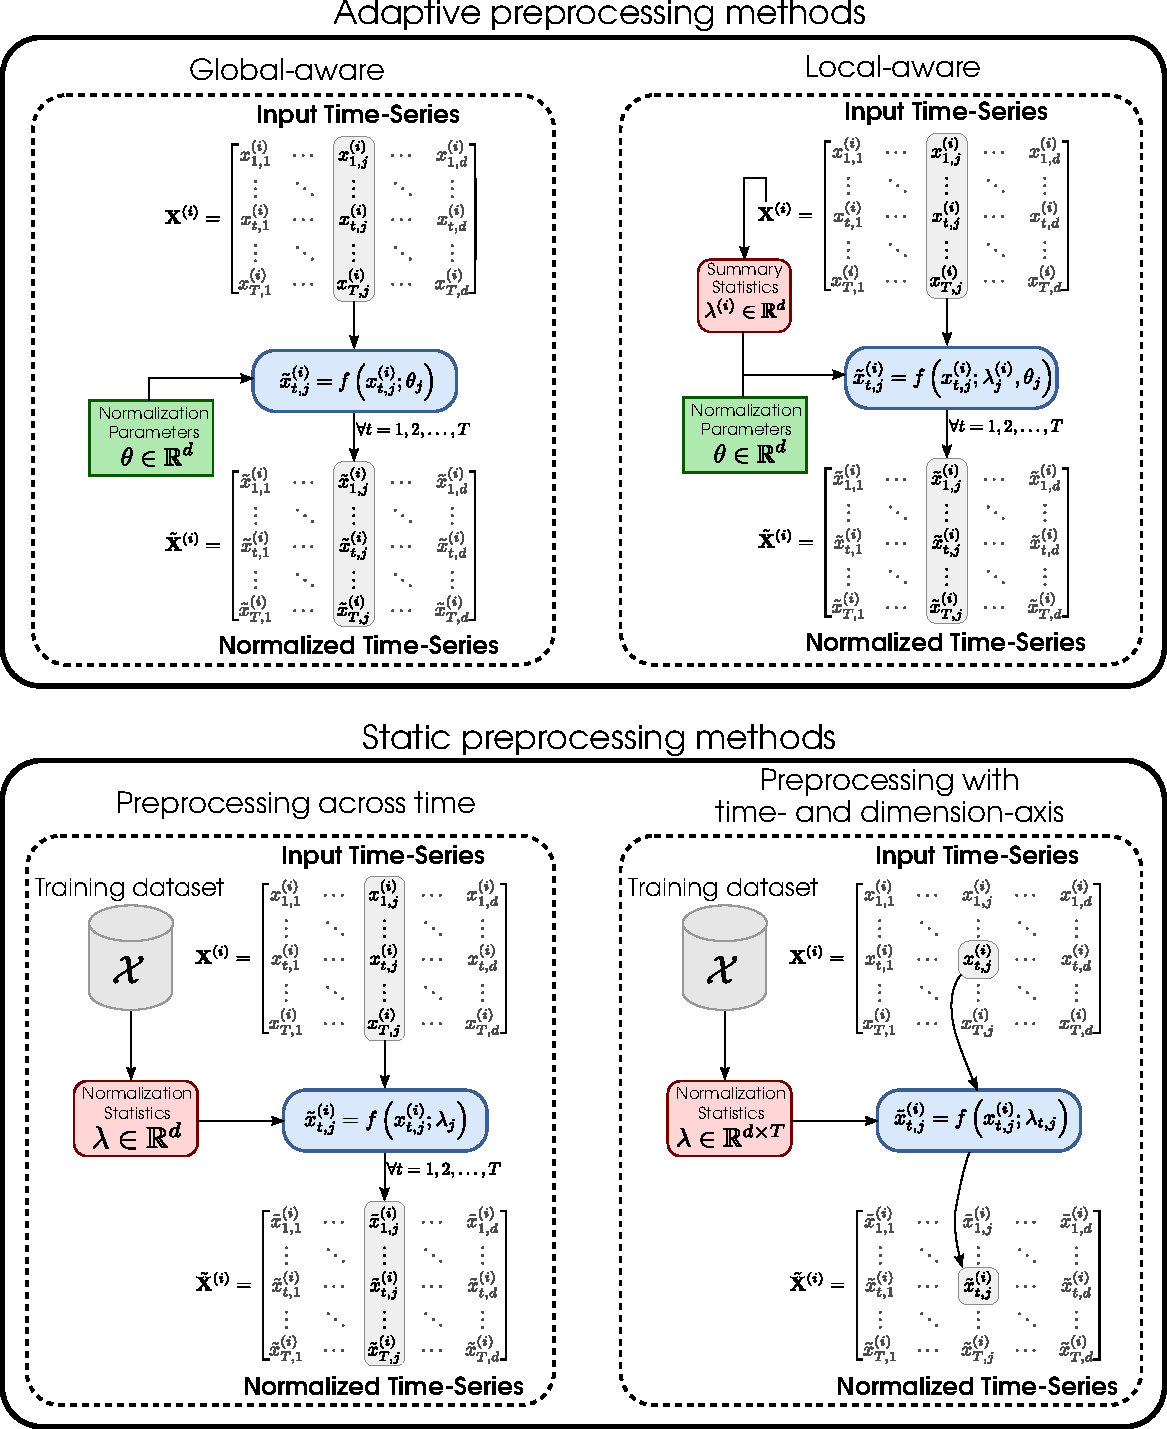
\includegraphics[width=\textwidth]{diagrams/local-vs-global-diagram.pdf}
    \end{center}
    \caption{The four different approaches to preprocessing a time-series sample. For the adaptive
        preprocessing methods, where the normalization parameters are learned with backpropagation, there
        are two types: local-aware and global-aware normalization. There are also two ways to apply
    static preprocessing methods, one across time and with both the time- and dimension-axis.}
    \label{fig:local_vs_global}
\end{figure}
% }}}

So far, we have only considered $d$-dimensional datasets, but when working with multivariate
time-series, there is also a temporal dimension, giving samples of the form
$\bfX \in \R^{d\times T}$. There are two approaches to applying the static
transformations in \cref{eq:pp1,eq:pp2,eq:pp3,eq:pp4,eq:pp5,eq:pp6,eq:pp7}
to such datasets, both of which are illustrated in the lower section of \cref{fig:local_vs_global}.
Say we are working with a transformation $\mathbf{f}: \R^d \rightarrow {\R^d}$, where the \textit{normalization statistics}, such as $\bm\mu$, $\bm\sigma$, $\bfx^{(min)}$, and $\bfx^{(max)}$, have been learned
from the dataset $\mathcal{D}$. The first approach, which I will refer to as
\textit{preprocessing across time}, involves merging the time-axis with the sample-axis, giving
an augmented dataset $\mathcal{D}'=\{\bfx^{(i\cdot T +t)}\}_{i=1,2,\dots,N,t=1,2,\dots,T}$
containing $N \cdot T$ samples, each of dimensionality $d$. This dataset $\mathcal{D}'$ is then
used to compute the normalization statistics $\bm\lambda \in \R^d$, and to transform each sample, we do
$\tilde{x}_{t,j}=f(x_{t,j};\lambda_j)$ for all $t=1,2,\dots,T$. In other words, we apply the same
transformation \textit{across time}.
%
In the second approach, which will be referred to as
\textit{preprocessing with time- and dimension-axis}, we do not augment the dataset. Instead,
we merge the time-axis and dimension-axis, and compute normalization statistics for
each of the $d \cdot T$ ``new features''. That is, we let
$\mathcal{D}''=\left\{\left[\bfx^{(i)}_{1} \; \bfx^{(i)}_{2} \; \cdots \; \bfx^{(i)}_{T} \right]^\top \right\}_{i=1,2,\dots,N}$ be our new dataset of $N$ samples, each $d\cdot T$-dimensional.
This gives normalization statistics on the form $\bm\lambda \in \R^{d\times T}$.
When transforming a data-point $x^{(i)}_{t,j}\in\R$, the transformation depends on both $j$ and $t$,
unlike the first method which only depended on $j$. This difference is illustrated
in \cref{fig:local_vs_global}.

% }}}


% Adaptive distribution transformation
\subsection{Adaptive distribution transformations}% {{{
\label{sub:Adaptive distribution transformations}

We now move onto the adaptive preprocessing techniques. The static
preprocessing techniques have unknown parameters that can be fully represented
by summary statistics, for instance the mean and standard deviation of the
training dataset. The adaptive preprocessing techniques, however, have unknown
parameters that need to be trained with the problem setting and neural network in
mind. As we see in \cref{fig:local_vs_global}, this makes the adaptive preprocessing methods
not rely on any normalization statistics directly computed from the training dataset.
That is, they are inferred in an end-to-end fashion. That way, the
preprocessing layers can \textit{adapt} to normalize the data in whatever
fashion is most suitable for the particular task and model architecture being used.


% DAIN layer subsection
\subsubsection{DAIN}% {{{
\label{ssub:DAIN}


% Talking about DAIN:
% * Main motivation is being able to handle nonstationarity of time-series,
%   that is mean and or variance might be a function of time
% * More on this..
% * Three sublayers:
%   * shift the data, which centres the the data in the feature space
%   * scaling, increase or reduce variances of samples, depending on what's most appopriate
%   * third layer performs gating, which is a non-linear operation that is able
%     to supress irrelvant features, that is, perform some notion of feature
%     selection
% * adaptive in the sense that the parameters can be trained on input data
% * local-aware in the sense that each normalization operation depends on the
%   current sample through summary aggregators. The normalization "adapts" to the
%   local distribution
% * Designed around application to financial forecasting problems, where dataset highly multimodal
% * local-aware normalization, which transforms all time-series into common representation space


The \acf{DAIN} layer, proposed by \cite{dain}, is one of the earliest preprocessing methods that can
handle highly multimodal and non-stationary multivariate time-series in an adaptive,
end-to-end fashion.
This layer was designed for financial forecasting tasks, where highly multi-modal
time-series are common. Additionally, these time-series are often non-stationary, that is, the
mean and variance of the data do not remain constant across time.
Both of these aspects makes Z-score normalization unsuitable as the statistics can differ
from one timestep to another, and Z-score scaling is not suitable on multimodal distributions.
The \ac{DAIN} layer handles these issues through three adaptive sublayers that all depend
on both summary statistics of the current time-series sample being normalized, as well as unknown normalization
parameters that are trained for the specific dataset and problem task considered.
As we see in \cref{fig:dain-arch}, the first sublayer is an adaptive shift layer
that centres the data. The second sublayer is an adaptive scaling layer that can increase or
reduce the variance of each sample. The third sublayer is a non-linear gating operation
that can suppress irrelevant features, that is, perform feature selection.


% To produce the diagram, run
%     pdfcrop --margins '-15 -30 0 -560' dain_paper_page2.pdf dain_diagram.pdf
% on the second page of a PDF copy of the DAIN paper by Passalis et al.
\begin{figure}
    \begin{center}
        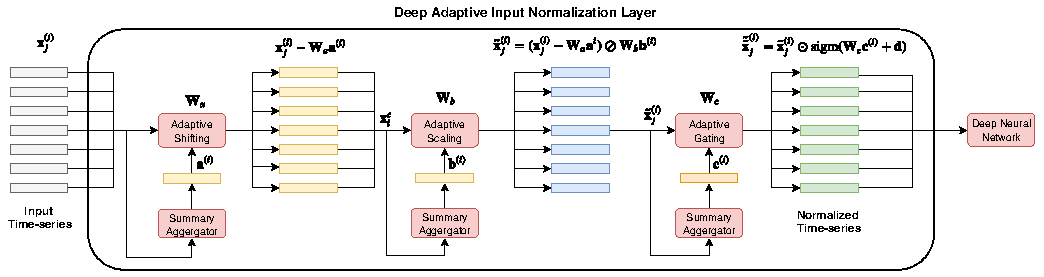
\includegraphics[width=\textwidth]{diagrams/dain_diagram.pdf}
    \end{center}
    \caption{Architecture of the \acf{DAIN} layer, proposed by \citeauthor{dain}. The diagram
    is taken from Figure 1 on page 2 of \cite{dain}.}
    \label{fig:dain-arch}
\end{figure}

Before delving deeper into how exactly the sublayers operate, we consider an illustrative
example of what might cause a high number of modes in financial data and why this might
be problematic for deep sequence models. In
\cite{dain}, the authors gives the example:
\begin{quote}
    ``\textit{[A]ssume two tightly
    connected companies with very different stock prices, e.g., 1\$
    and 100\$ respectively. Even though the price movements can
    be very similar for these two stocks, the trained forecasting
    models will only observe very small variations around two
    very distant modes (if the raw time series are fed to the model).}''
\end{quote}
Therefore, the time-series are normalized in what I will refer to as a
\textit{local-aware} fashion, that is, the transformation applied also depends
on summary statistics
computed from  the particular time-series being normalized. This local-aware method of normalization
is illustrated in \cref{fig:local_vs_global}, and it allows
the amount of shifting and scaling to also depend on the particular mode in the dataset the sample
came from, and this information can then be discarded.
This enables transforming all the samples into a common more unimodal
representation space, despite the input data being highly multimodal.
Illustrative plots of this phenomenon are presented later in the thesis in
\cref{sub:local_vs_global}.

We now look more closely at  the \ac{DAIN} architecture, of which an overview is shown
in \cref{fig:dain-arch}. The unknown parameters are the weight matrices
$\mathbf{W}_a$, $\mathbf{W}_b$, $\mathbf{W}_c \in \R^{d \times d}$, and the bias
term $\mathbf{d} \in \R^d$, and are used
for the shift, scale, and gating sublayer, respectively. The adaptive shift layer and
adaptive scale layer, together, perform the operation
\begin{equation}\label{eq:dain_tild}
    \tilde{\bfx}_t^{(i)}=\left(
        \bfx_t^{(i)}-\mathbf{W}_a \mathbf{a}^{(i)}
    \right) \oslash \mathbf{W}_b \mathbf{b}^{(i)},
\end{equation}
where $\mathbf{a}^{(i)}$ and $\mathbf{b}^{(i)}$ are summary statistics that are computed for
the $i$th sample as follows:
\begin{align}
    \mathbf{a}^{(i)}& =\frac{1}{T} \sum^{T}_{t=1} \bfx_t^{(i)}, \label{eq:dain_a}\\
    b_k^{(i)}&=\sqrt{
    \frac{1}{T} \sum^{T}_{t=1} \left(x^{(i)}_{t,k} - \left[\mathbf{W}_a  \mathbf{a}^{(i)}\right]_k \right)^2},
    \qquad k=1,2,\dots,d. \label{eq:dain_b}
\end{align}
The third sublayer, the gating layer, performs the operation
\begin{equation}
    \tilde{\tilde{\bfx}}_t^{(i)}=\tilde{\bfx}^{(i)} \odot \textrm{sigm}\left( \mathbf{W}_c \mathbf{c}^{(i)} + \mathbf{d}\right),
\end{equation}
where $\textrm{sigm}(\cdot)$ denotes the sigmoid function, defined as
$\textrm{sigm}(x)=1/(1+e^{-x})$, and $\mathbf{c}^{(i)}$ is the third summary statistic, computed
with
\begin{equation}
    \mathbf{c}^{(i)}=\frac{1}{T} \sum^{T}_{t=1} \tilde{\bfx}_t^{(i)}.
\end{equation}

% }}}

% RDAIN layer subsection
\subsubsection{RDAIN}% {{{
\label{ssub:RDAIN}

% RDAIN:
% * By same author as DAIN paper, extends it with a residual connection
% * Additionally, introduce bias terms
% * Show diagram
A few years after \citeauthor{dain} proposed the \ac{DAIN} layer in \citeyear{dain}, they
improved on
this layer with the \acf{RDAIN} architecture \citep{rdain}. This adaptive preprocessing layer
extends \ac{DAIN} with a local-aware residual connection that skips the adaptive shift and
scale sublayers. Additionally, the adaptive shift and scale sublayers in \ac{RDAIN} also
include a trainable bias term, not just a weight matrix.

% \begin{equation}
%     \bm\alpha(\bfx)=\mathbf{W}_\alpha \mathbf{s}_\alpha(\bfx) + \mathbf{b}_\alpha \in \R^d
% \end{equation}
% \begin{equation}
%     \bm\beta(\bfx)=\left(\mathbf{W}_{\beta} \mathbf{s}(\bfx)+\mathbf{b}_\beta \right)^{-1}
% \end{equation}
% \begin{equation}
%     \gamma(\bfx)=\textrm{sigm}\left(\mathbf{W}_\gamma \mathbf{s}_\gamma(\bfx)+\mathbf{b}_\gamma \right)
% \end{equation}


% }}}

% BIN layer
\subsubsection{BiN}% {{{
\label{ssub:BiN}


% BIN:
% * Also uses "sample-level statistics" to adapt to the local distribution
% * Performs similar operation as DAIN layer, but does it across both time and dimension axis,
%   then it combines the two results with a linear combination
% * Using the same notation is with DAIN, the operation is
% * TODO: equations for the operations, such that easy to understand ....
%   * Do this while reading the BIN paper

The third adaptive preprocessing method is the \acf{BIN} layer, initially
presented by \cite{bin}. It has a similar architecture to \ac{DAIN}, but drops the
third gating layer. Additionally, while the \ac{DAIN} only does an adaptive shift and scale layer
based on a summary representation computed from a sum along the time-axis, the \ac{BIN} layer
does a similar operation twice, once across the time-axis, and once across the dimension-axis.
It then returns a linear combination of these two normalized time-series as the
final output. Visually, this can be thought of as performing the local-aware normalization
shown in \cref{fig:local_vs_global} two times, once for $\bfX^{(i)}$ and once for its transpose,
and outputting trainable a linear combination of the two.

We now look at the adaptive scale- and shift sublayers of the \ac{BIN} architecture.
Recall that one sample is a multivariate time-series of the form $\bfX^{(i)} \in \R^{d \times T}$.
Like the \ac{DAIN} layer in \cref{eq:dain_a,eq:dain_b}, the \ac{BIN} layer also
computes two summary representations of each sample along the time-\textit{column}:
\begin{align}
    \overline{\mathbf{c}}^{(i)}& =\frac{1}{T} \sum^{T}_{t=1} \bfx_t^{(i)} \in \R^d, \\
    \bm\sigma_c^{(i)}&=\sqrt{
    \frac{1}{T} \sum^{T}_{t=1} \left(\bfx^{(i)}_{t} - \overline{\mathbf{c}}^{(i)} \right)
    \odot \left(\bfx^{(i)}_{t} - \overline{\mathbf{c}}^{(i)} \right)
} \in \R^d.
\end{align}
These summary representation are then used together with unknown parameters
$\bm\gamma_c \in \R^d$ and $\bm\beta_c \in \R^d$ to produce a sample that is normalized across
the time-\textit{column}:
\begin{equation}
    \tilde{\bfx}^{(i)}_t= \bm\gamma_c \odot \left\{
        \left(\mathbf{x}^{(i)}_t - \overline{\mathbf{c}}^{(i)}\right)\oslash \bm\sigma_c^{(i)}
    \right\}+\bm\beta_c, \qquad \forall t=1,2,\dots,T.
\end{equation}
Note that the multiplication order of the unknown parameters differ from what
\ac{DAIN} does in \cref{eq:dain_tild}, where the summary representations and unknown parameters
are first multiplied together before being used to transform the sample.
Similarly, along the dimension-\textit{row}, we compute
the summary representations:
\begin{align}
    \overline{\mathbf{r}}^{(i)}& =\frac{1}{d} \sum^{d}_{k=1} \bfx_{*,k}^{(i)} \in \R^T, \\
    \bm\sigma_r^{(i)}&=\sqrt{
        \frac{1}{d} \sum^{d}_{k=1} \left(\bfx^{(i)}_{*,k} - \overline{\mathbf{r}}^{(i)} \right)
        \odot \left(\bfx^{(i)}_{*,k} - \overline{\mathbf{r}}^{(i)} \right)
    } \in \R^T.
\end{align}
The row-summaries are then used together with new unknown parameters
$\bm\gamma_r \in \R^T$ and $\bm\beta_r \in \R^T$ to produce
a sample that is normalized across the dimension-\textit{row}:
\begin{equation}
    \tilde{\tilde{\bfx}}^{(i)}_{*,k}= \bm\gamma_r \odot \left\{
        \left(\mathbf{x}^{(i)}_{*,k} - \overline{\mathbf{r}}^{(i)}\right)\oslash \bm\sigma_r^{(i)}
    \right\}+\bm\beta_r, \qquad \forall k=1,2,\dots,d.
\end{equation}
The output of the \ac{BIN} layers is then a linear combination of these two normalized samples:
\begin{equation}
    \textrm{BIN}_{OUTPUT}\left( x_{t,k}^{(i)}\right)
    = \lambda_c \tilde{x}^{(i)}_{t,k} + \lambda_r \tilde{\tilde{x}}^{(i)}_{t,k},
\end{equation}
where $\lambda_c \in \R$ and $\lambda_r\in\R$ are two learnable scalars that allows the \ac{BIN} layer
to learn how much to weigh each of the normalization methods.


% }}}


% END adaptive layer }}}


% END data preprocessing }}}

\section{Conclusion}% Conclusion
\label{sec:Conclusion}% {{{

% Deep learning:
% * Linear layer, works by multiplying post-activations from previous layer with
%   weight matrix and bias term, then passed through activation function,
% * training NN using stochastic gradient descent, where pass one batch of
%   samples at the time and look at the average gradient of the loss with respect
%   to unknown parameters,
% * iteratively update the parameter values based on this gradient with a learning rate
% * also covered early stoppers for imrpvoing generalization performance, and
%   lr scheduler for more stable convergence
% * Then moved onto sequence model and described the basic RNN cell as well as the GRU cell
In this chapter, we provided an overview of deep learning and various data preprocessing techniques
suitable for multivariate time-series. We looked at the linear neural network layer, which
produces pre-activations that are weighted sums of the previous post-activations and bias terms.
These are then passed through a non-linear activation function to produce the next vector of
post-activations. We also looked at training a neural network with stochastic gradient descent,
where the gradients of the loss with respect to the unknown parameters are estimated on a batch of
data using backpropagation. The gradient estimates are then used to iteratively update the model
parameters until a certain number of epochs have elapsed. We also looked at using early stopping,
learning rate scheduling and adaptive optimizers to make the training process more efficient and
stable, as well as improving generalization performance. Finally, we covered some common building
blocks used in deep sequence models.

% * data preprocessing.Covered static distribution transformations such as min-max, Z-score
%   scaling, Z-score scaling with tanh activation function, decimal scaling,
%   the Box-Cox transformation for handling skewed data, and winsorization for
%   handling outliers
% * computed using statistics to estimate the mean, standard deviation, minimum, maximum, etc.
% * then moved onto adaptive preprocessing techniques, such as the DAIN, RDAIN, BIN
% * DAIN consists of an adaptive scale and shift layer, followed by an adaptive
%   gating layer used for feature selection. The BIN layer similarly contains an adaptive scale
%   and shift layer, and applies this along both the time-axis and dimension-axis and returns
%   a learned linear combination of these, while the DAIN layer only summary representation along
%   time-axis
We then looked at the most commonly used data preprocessing techniques, which are mostly static
distribution transformations such as min-max scaling, Z-score scaling, Z-score scaling with a
$\tanh$ activation function, decimal scaling, the Box-Cox transformation for handling skewed data,
and winsorization for handling outliers. All of these techniques use normalization
statistics such as the
mean, the standard deviation, etc.\ to compute the transformation parameters. We then looked at
another more recent class of preprocessing techniques: adaptive preprocessing methods.
We considered \ac{DAIN}, \ac{RDAIN}, and \ac{BIN}, which were proposed by
\cite{dain,rdain,bin}, respectively. These three adaptive preprocessing
methods have trainable parameters that are optimised together with the neural
network instead of using normalization statistics. They are also all local-aware, meaning that they use
a summary representation of each sample to adjust the extent at which the normalization is applied
to each sample. The \ac{BIN} method does this over both the time- and dimension-axis while the
\ac{DAIN} method only uses summary representations computed by summing over the time-axis.

% }}}

%%%%%%%%%%%%%%%%%%%%%%%%%%%%%%%%%%%%%%%%%%%%%%%%%
\chapter{Methods} %%%%       METHODS         %%%%
%%%%%%%%%%%%%%%%%%%%%%%%%%%%%%%%%%%%%%%%%%%%%%%%%
\label{ch:Methods}

% Introduction
% Introduction {{{
In this chapter, I present the main contributions of this thesis: three novel
preprocessing methods. The first method, abbreviated \acs{EDAIN}, is based on
existing work by \cite{dain} and \cite{bin}. It is an adaptive
preprocessing method, so it performs a sequence of parametrised transformations
on the input data before passing it to a deep neural network. To optimize the
adaptive layer, the deep neural network is augmented with the \acs{EDAIN} layer
and both the neural network parameters and the \acs{EDAIN} parameters are
trained with stochastic gradient descent.  In \cref{sec:EDAIN-KL-method}, I
present the second method, abbreviated \acs{EDAIN-KL}.  This method uses a very
similar architecture to the \acs{EDAIN} layer, but instead of fitting the
parameters using stochastic gradient descent, it is optimised with a technique
inspired by \textit{normalizing flow} networks. In
\cref{sec:PREPMIX-CAPS-method}, my third contribution, the \acs{PREPMIX-CAPS}
procedure, is presented. This procedure is fundamentally different from the
first two methods, as it automatically selects a mixture of static
preprocessing techniques to apply to the data instead of using adaptive
transformations.

% }}}

\section{EDAIN}% EDAIN
% Methods: EDAIN {{{
\label{sec:EDAIN-method}

% Topics of this section:
% * Illustrative diagram of the 4 layers, and the weights, justifying order of operations
% * Differences to DAIN, explaining batch awareness, and specifics of (amex) dataset worked with
% * Explaining the 3 parts:
%   * outlier removal: Inspired by winsorization, plot of curve for different values,to show how work
%   * scale&shift: able to generalise standard scaling
%   * power transform: should also work for negative and positive values, while being numerically stable

My first contribution is the \acf{EDAIN} layer. This adaptive preprocessing layer is inspired
by \ac{DAIN} and \ac{BIN}, from work by \cite{dain} and \cite{bin}, respectively. However,
unlike their adaptive preprocessing methods, the
\ac{EDAIN} layer also supports normalizing the data in a \textit{global-aware} fashion, whereas
the \ac{DAIN}, \ac{RDAIN} and \ac{BIN} layers are all \textit{local-aware}.
The \ac{EDAIN} layer has four different sublayers. The first sublayer reduces the effect of
outliers in the data, while the second and third sublayer perform an adaptive shift and
scale operation. Finally, an adaptive power transform operation is applied to reduce the
skewness of the input data.

\subsection{Architecture}%
\label{sub:edain_arch}

% Latex equations used:
% \(\mathbf{\alpha}' \odot \left(\mathbf{\beta}' \odot \tanh\left\{(\mathbf{x}_t^{(i)}-\hat{\mathbf\mu}) \oslash \mathbf{\beta}'  \right\}+\hat{\mathbf\mu} \right)+\left(1-\mathbf{\alpha}' \right) \odot \mathbf{x}_t^{(i)}\)
% \((\mathbf{\tilde{x}}_t^{(i)}  - \mathbf{\gamma} \mathbf{\mu}_{\mathbf{\tilde{x}}_t^{(i)}}) \oslash \mathbf{\lambda} \sigma_{\mathbf{\tilde{x}}_t^{(i)}}, \textrm{ if local-aware} \)
% TODO: add w=(alpha, beta) above the red boxes to highlight which parameters are optimized...
\begin{figure}
\begin{center}
    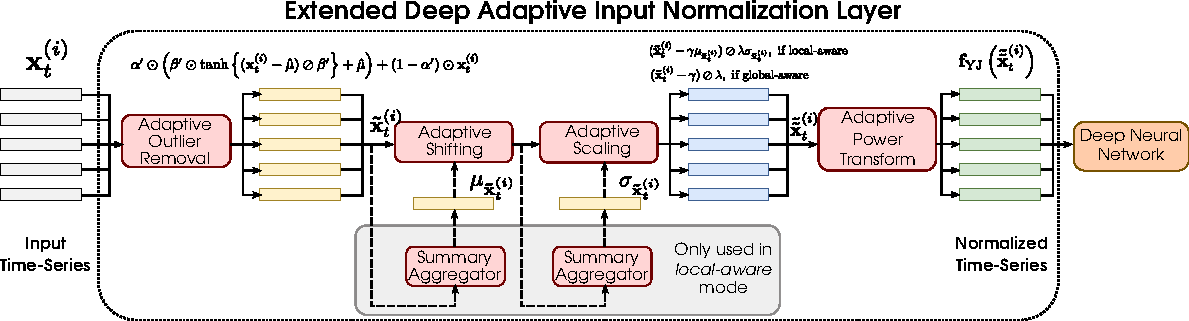
\includegraphics[width=\textwidth]{diagrams/edain-diagram.pdf}
\end{center}
\caption{An overview of the architecture of the proposed \ac{EDAIN} normalization layer. The
style and colours chosen in the diagram is inspired by Figure 1 in \cite{dain}.}
\label{fig:edain-arch}
\end{figure}

An overview of the layer's architecture is shown in \cref{fig:edain-arch}.
Given some input time-series $\bfX^{(i)} \in \R^{d \times T}$, each temporal segment
$\bfx^{(i)}_t$ is passed through an adaptive outlier removal layer $\mathbf{h}_1$, followed by an adaptive shift operation $\mathbf{h}_2$, an adaptive scale operation $\mathbf{h}_3$, and then
finally through an adaptive power transformation layer $\mathbf{h}_4$.
The architecture also has two modes, \textit{local-aware} and \textit{global-aware}.
In
global-aware mode, the \ac{EDAIN} layer applies the same operation to each time-series such
that the relative order in the ``global distribution'' is maintained.
In local-aware mode,
the \ac{EDAIN} layer's normalization operations
also depend on summary statistics of each input time-series $\bfX^{(i)}$, which allows to normalize
each mode  in the data differently,
independent of where in the ``global distribution'' the sample originated from.
The high-level difference between these two
modes of adaptive normalization is shown in \cref{fig:local_vs_global}.
The local-aware mode is most suitable for
multi-modal input data, as samples from different modes can all be transformed into one common
normalized unimodal representation space. On the other hand, the global-aware mode
is most suitable if all the data comes from a similar data generation mechanisms,
and works best if the input data has few modes.
In local-aware mode, the \ac{EDAIN} architecture is similar to the
\ac{DAIN} architecture proposed by \cite{dain} and shown
in \cref{fig:dain-arch}, but it
extends it with an adaptive outlier removal sublayer and an adaptive power transform sublayer.
The global-aware mode was not considered by \cite{dain} and is one of our contributions.

% Outlier removal
\subsubsection{Outlier removal}% {{{
\label{ssub:Outlier removal}

Treating outliers and extreme values in our dataset can increase predictive performance if done
correctly \citep{outlier_wind}.
Two common ways of doing this are omission and winsorization
\citep{winsorization}. With the former, observations that are deemed to be extreme are simply
removed during training. With the latter, all the data is still used, but observations lying
outside a certain number of standard deviations from the mean, or below or above certain
percentiles, are \textit{clipped} to be closer to the mean or median of the data. We refer to this
technique as \textit{winsorization}.
For example, if winsorizing data using three standard deviations, all values less than
$\mu-3\sigma$ are set to be exactly $\mu-3\sigma$. Similarly, the values above
$\mu+3\sigma$ are clipped to this value. Winsorization can also be done using percentiles,
where common boundaries are the first and fifth percentiles \citep{winsorization}.
However, the type of winsorization, as well as the number of standard deviations
or percentiles to use, might depend on the dataset. Additionally, it might not
be necessary to winsorize the data at all if the outliers turn out to not
negatively affect performance. All this introduces more hyperparameters to tune
during modelling. The outlier removal operation presented here aims to automatically  determine both
whether winsorization is necessary for a particular feature, and determine the threshold at
which to apply winsorization.

For input vector $\bfx_t^{(i)} \in \R^d$, the adaptive outlier removal operation is defined as:
\begin{equation}\label{eq:adaptive-outlier-removal}
    \mathbf{h}_1\left(\bfx_t^{(i)}\right)=\bm\alpha' \odot \underbrace{\left(\bm\beta' \odot
        \tanh\left\{\left(\bfx_t^{(i)}-\hat{\bm\mu}\right) \oslash \bm\beta'  \right\}+\hat{\bm\mu}
\right)}_{\text{smooth adaptive centred winsorization}}
    +\underbrace{\left(1-\bm\alpha' \right) \odot \bfx}_{\text{residual connection}},
\end{equation}
where
$\bm\alpha' \in [0,1]^d$ is a parameter controlling how much winsorization to apply to each feature,
and $\bm\beta' \in [\beta_{\text{min}},\infty)^d$ controls the winsorization threshold for
each feature, that is, the maximum absolute value of the output, thus controlling the range of the
output. The effect of the two parameters is illustrated in \cref{fig:adaptive_outlier}.
The unknown parameters of the model are $\bm\alpha \in \R^d$ and $\bm\beta \in \R^d$, and they
are transformed into the constrained parameters $\bm\alpha'$ and $\bm\beta'$, as used in
\cref{eq:adaptive-outlier-removal}, through the following  mappings:
\begin{equation}
    \bm\alpha'=\frac{e^{\bm\alpha}}{1\oplus e^{\bm\alpha}} \qquad\qquad
    \bm\beta'=\beta_{\text{min}}\oplus e^{\bm\beta},
\end{equation}
where $\beta_{\textrm{min}} \in \R$ is a hyperparameter that can be tuned, but a suitable value is $\beta_{\textrm{min}}=1$. We introduce $\beta_{\textrm{min}}>0$ to prevent the sublayer from
squeezing all the data into the range $[0,0]$ during training, as the smallest possible range
with the parameter becomes $[-\beta_{\textrm{min}}, \beta_{\textrm{min}}]$.


The $\hat{\bm\mu}\in \R^d$ vector in \cref{eq:adaptive-outlier-removal} is an estimate of the mean of the data, and is used
to ensure the winsorization is centred. When setting the \ac{EDAIN} layer in \textit{local-aware}
mode, it is simply the mean of the current time-series sample:
\begin{equation}
    \hat{\bm\mu}=\frac{1}{T} \sum_{t=1}^T \bfx_{t}^{(i)}. %, \qquad k=1,\dots,d.
\end{equation}
In global-aware mode, it is iteratively updated using a \textit{cumulative
moving average estimate} at each forward pass of the sublayer.
This is to better approximate the global mean of the data.
With this approach, we simply keep track of the current estimated average at forward pass $i$,
denoted $\hat{\bm\mu}^{(i)}$, and update it with
\begin{equation}
    \hat{\bm\mu}^{(i+1)}= \frac{iT\cdot\hat{\bm\mu}^{(i)}+\sum^{T}_{t=1} \bfx_t^{(i)}}{(i+1)T}
\end{equation}
when the sublayer receives a new time-series $\bfX^{(i)}\in\R^{d\times T}$. We also initialise
$\hat{\bm\mu}^{(0)}=\mathbf{0}$.

\begin{figure}
\begin{center}
    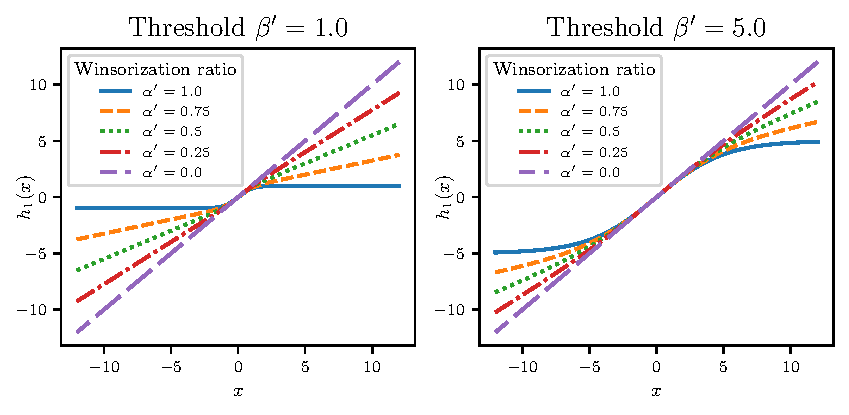
\includegraphics[width=\textwidth]{figures/adaptive_outlier_removal.pdf}
\end{center}
\caption{Plot of the adaptive outlier removal operation for different combinations of parameter
values for $\alpha'$ and $\beta'$.}
\label{fig:adaptive_outlier}
\end{figure}


% }}}

% Scale and shift
\subsubsection{Scale and shift}% {{{
\label{ssub:Scale and shift}

Depending on the dataset, one might want to aim for a \textit{global
normalization}, in which case a \textit{global-aware} scale and shift operation is most
suitable. If the dataset has many different modes, with significantly different distribution characteristics, a \textit{local normalization} based on the specific mode each data point comes from is more suitable, in which case a \textit{local-ware} scale and shift
operation works best. This gives two different approaches to scaling and
shifting the data in an adaptive fashion, both illustrated in \cref{fig:local_vs_global}.

\paragraph{Global-aware}%
\label{par:Global-aware}

In global-aware mode, the adaptive shift and scale layer, combined, simply perform the operation
\begin{equation}\label{eq:adaptive-scale-shift}
    \mathbf{h}_3\left(\mathbf{h}_2\left(\bfx_t^{(i)}\right)\right)=(\bfx_t^{(i)} - \bm\gamma) \oslash \bm\lambda,
\end{equation}
where the unknown parameters are $\bm\gamma \in \R^d$ and $\bm\lambda \in (0,\infty)^d$.
This makes the scale-and-shift layer a generalised version of
Z-score scaling, or standard scaling, as setting
\begin{equation}
    \bm\gamma=\frac{1}{N T}  \sum^{N}_{i=1} \sum^{T}_{t=1} \bfx_{t}^{(i)}
\end{equation}
and
\begin{equation}
    \bm\lambda=\frac{1}{N T} \sum^{N}_{i=1} \sum^{T}_{t=1} \left(\bfx_{t}^{(i)}- \bm\gamma\right)^2
\end{equation}
makes the operation in \cref{eq:adaptive-scale-shift} equivalent applying Z-score scaling
across time.
This global-aware mode is useful if the distribution is similar across samples
and resembles a global unimodal distribution that should be standardized, as the operation
can generalise Z-score scaling.

\paragraph{Local-aware}%
\label{par:Local-aware}

Some datasets might have multiple modes arising from significantly different
data generation mechanisms. Attempting to scale and shift each time-series sample
by the same amount, according to some global mean and
standard deviation, might hurt performance in such a case. Instead, \cite{dain} propose
basing the scale and shift on a \textit{summary representation} of each data point, allowing
each time-series to be normalized according the specific mode of the data it originated from.
We define
\begin{equation}
    \mathbf{h}_3\left(\mathbf{h}_2\left(\bfx_t^{(i)}\right)\right)=
    \left(\bfx_t^{(i)} - \left[\bm\gamma \odot \mu_{\bfx}^{(i)}\right]\right) \oslash \left[\bm\lambda \odot \sigma_{\bfx}^{(i)}\right],
\end{equation}
where the summary representations $\sigma_{\bfx}^{(i)} \in \R^d$ and $\mu_{\bfx}^{(i)} \in \R^d$,
which as shown in \cref{fig:local_vs_global},  are computed through a reduction
along the temporal dimension of each observation $\bfX^{(i)}$:
\begin{align}
    \mu_\bfx^{(i)}&=\frac{1}{T} \sum^{T}_{t=1} \bfx^{(i)}_t  \\
    \sigma_\bfx^{(i)}&=\sqrt{\frac{1}{T}  \sum^{T}_{t=1} \left(\bfx^{(i)}_t- \mu_\bfx^{(i)} \right)^2}.
\end{align}
With this mode, it is difficult for the layer to generalise Z-score scaling, but it allows
discarding mode information such that highly multimodal distributions become unimodal after 
being transformed by the preprocessing layer.

% }}}

% Power transform
\subsubsection{Power transform}% {{{
\label{ssub:Power transform}

Many real-world datasets exhibit significant skewness, which is often treated using power
transformations \citep{skewed_data}.
The most common transformation is the Box-Cox transformation,
but this is only valid for positive values, so it is not applicable to most real-world datasets
\citep{boxcox}. An alternative is the transformation proposed by \cite{yeoJohnson},
known as the Yeo-Johnson transform:
\begin{equation}\label{eq:yeo-johnson}
    f_{\textrm{YJ}}^\lambda(x)= \left\{
        \begin{array}{ll}
            \frac{(x+1)^{\lambda}-1}{\lambda}, & \textrm{if } \lambda \neq 0, x \geq 0; \\
            \log(x + 1), & \textrm{if } \lambda = 0, x \geq 0;  \\
            \frac{(1-x)^{2-\lambda}-1}{\lambda-2} , & \textrm{if } \lambda \neq 2, x < 0; \\
            -\log(1-x), & \textrm{if } \lambda=2, x < 0.
        \end{array}
    \right.
\end{equation}
Like the Box-Cox transformation, the transformation $f_{\textrm{YJ}}$ only has one unknown parameter, $\lambda$, but
it works for any $x \in \R$, not just positive values \citep{yeoJohnson}.
The power transform layer simply applies the transformation in
\cref{eq:yeo-johnson} along each dimension of the input. That is, for each
$i=1,\dots,N$ and $t=1,\dots,T$, we define
\begin{equation}
    \left[\mathbf{h}_4\left(\bfx_t^{(i)}\right)\right]_j=f^{\lambda_j^{(\textrm{YJ})}}_{\textrm{YJ}}\left(x_{t,j}^{(i)}\right), \;\;\; j=1,\dots,d.
\end{equation}
The vector of the $d$ unknown parameter for the Yeo-Johnson transformation will be
denoted $\bm\lambda^{(\textrm{YJ})} \in \R^d$, as to not be confused with the scale parameter
$\bm\lambda \in \R^d$.


% }}}

% Optimising the parameters
\subsection{Optimisation through stochastic gradient descent}% {{{
\label{sub:edain_opt_sgd}

To optimise the unknown parameters
$\left( \bm{\alpha}, \bm{\beta}, \bm{\gamma}, \bm{\lambda}, \bm{\lambda}^{(\textrm{YJ})}\right)$,
the deep neural network is augmented by prepending the \ac{EDAIN} layer, as shown in
\cref{fig:edain-arch}. Then the input data is fed into the augmented model in batches,
as when training a neural network, and after each forward pass of the model, the weights
are updated through stochastic gradient descent while training the neural network.
As observed by \cite{dain}, the model convergence is unstable if the same learning rate
$\eta \in \R$ that is used for training the deep neural network is also used for training all
the sublayers of the adaptive preprocessing layer. Therefore, separate learning rate modifiers
$\eta_{\textrm{out}}$,
$\eta_{\textrm{shift}}$,
$\eta_{\textrm{scale}}$ and
$\eta_{\textrm{pow}}$ for the outlier removal, shift, scale and power transform sublayers are
introduced as additional hyperparameters. The parameter updates happen according to the equation:
\begin{equation}
    \Delta \left( \bm{\alpha}, \bm{\beta}, \bm{\gamma}, \bm{\lambda}, \bm{\lambda}^{(\textrm{YJ})}\right)
    =
    -\eta\left(
        \eta_{\textrm{out}} \frac{\partial \mathcal{L}}{\partial \bm\alpha},
        \eta_{\textrm{out}} \frac{\partial \mathcal{L}}{\partial \bm\beta},
        \eta_{\textrm{shift}} \frac{\partial \mathcal{L}}{\partial \bm\gamma},
        \eta_{\textrm{scale}} \frac{\partial \mathcal{L}}{\partial \bm\lambda},
        \eta_{\textrm{pow}} \frac{\partial \mathcal{L}}{\partial \bm{\lambda}^{(\textrm{YJ})}}
    \right),
\end{equation}
where $\mathcal{L}$ denotes the criterion evaluated at a batch of inputs and targets, and
$\eta \in \R^+$ is the base learning rate.


% }}}

% }}}

\section{EDAIN-KL}% EDAIN-KL
% Methods: EDAIN-KL {{{
\label{sec:EDAIN-KL-method}

The \ac{EDAIN-KL} layer has a very similar architecture to the earlier-presented
\ac{EDAIN} layer, but the unknown parameter are optimised in a completely different
manner. Unlike the \ac{EDAIN} layer, the \ac{EDAIN-KL} layer is not attached to the deep neural
network during training and thus not trained simultaneously with the neural network. Instead,
before training the neural network, we train the \ac{EDAIN-KL} layer in isolation.
This is done by using it to transform a standard
normal distribution into a distribution that is similar to our training dataset. Then, after
the \ac{EDAIN-KL} weights have been optimized, we use the layer in reverse to normalize samples
from the training dataset before passing it to the neural network.

\subsection{Architecture}%
\label{sub:Architecture}

The \ac{EDAIN-KL} layer has a very similar architecture to the \ac{EDAIN} layer, described in
\cref{sec:EDAIN-method}, but the outlier removal transformation has been simplified to ensure its
inverse is analytic. Additionally, the layer no longer supports local-aware mode, as this
would make the inverse intractable. The \ac{EDAIN-KL} transformations are:
\begin{align}
    \textrm{(Outlier removal)} \qquad& \mathbf{h}_1\left(\bfx^{(i)}_t\right)=\bm\beta' \odot \tanh\left\{(\bfx^{(i)}_t - \hat{\bm\mu}) \oslash \bm\beta' \right\}+\hat{\bm\mu} \label{eq:kl1}\\
    \textrm{(shift)} \qquad& \mathbf{h}_2\left(\bfx^{(i)}_t\right)=\bfx^{(i)}_t- \bm\gamma \label{eq:kl2}\\
    \textrm{(scale)} \qquad& \mathbf{h}_3\left(\bfx^{(i)}_t\right)=\bfx^{(i)}_t \oslash \bm\lambda  \label{eq:kl3}\\
    \textrm{(power transform)} \qquad& \mathbf{h}_4\left(\bfx^{(i)}_t\right)=\left[
        f^{\lambda_1^ {(\textrm{YJ})} }_{\textrm{YJ}}\left(x^{(i)}_{t,1}\right),
        % \quad f^{\lambda_2^ {(\textrm{YJ})}}_{\textrm{YJ}}\left(x^{(i)}_{t,1}\right)
        \quad \cdots,
        \quad f^{\lambda_d^ {(\textrm{YJ})}}_{\textrm{YJ}}\left(x^{(i)}_{t,d}\right)
    \right], \label{eq:kl4}
\end{align}
where $f^{\lambda_i^ {(\textrm{YJ})}}_{\textrm{YJ}}(\cdot)$ is defined in \cref{eq:yeo-johnson}.

\subsection{Optimisation through Kullback-Leibler divergence}%
\label{sub:opt_with_kl}

The  optimisation approach used to train the \ac{EDAIN-KL} method is inspired by normalizing flows,
of which \cite{normalizing_flows} provide a great overview of.
Before describing the approach, we provide a brief overview of related notation and some
background on the concept behind normalizing flows. After this, we go through how the
\ac{EDAIN-KL} layer itself can be treated as an invertible bijector to fit into the
normalizing flow framework. In doing so, we realize the need for analytic and differentiable
expressions for certain terms related to the \ac{EDAIN-KL} layer. Derivations for these terms are
then presented.

\subsubsection{Brief background on normalizing flow}%
\label{ssub:Brief background on normalizing flow}

The idea behind normalizing flows is taking a simple random variable, such as a standard
Gaussian, and transforming it into a more complicated distribution, for example, one that
resembles the distribution of a given dataset of samples.
Consider a random variable $\bfZ \in \R^d$ with a known and
analytic expression for the \ac{pdf} $p_\bfz: \R^d \rightarrow {\R}$. We refer to $\bfZ$ as
the \textit{base distribution}. We then define
a parametrised invertible function
$\mathbf{g}_{\bm \theta}:\R^d \rightarrow {\R^d}$, also known as a \textit{bijector},
and use this to transform the base distribution into a new
 probability distribution: $\bfY=\mathbf{g}_{\bm\theta}(\bfZ)$.
By increasing the complexity of the bijector $\mathbf{g}_{\bm\theta}$, by for instance using
a deep neural network, the transformed distribution $\bfY$ can grow arbitrarily complex as well.
The \ac{pdf} of the transformed distribution can then be computed using the change of variable
formula \citep{normalizing_flows}, where
\begin{align}
    p_\bfY(\bfy)&=p_\bfZ(\mathbf{g}_{\bm\theta}^{-1}\left(\bfy\right))\cdot \left|\det \mathbf{J}_{\bfY \rightarrow {\bfZ}}\left(\bfy \right) \right| \nonumber \\
                & = p_\bfZ(\mathbf{g}_{\bm\theta}^{-1}\left(\bfy\right))\cdot \left|\det \mathbf{J}_{\bfZ \rightarrow {\bfY}}\left( \mathbf{g}^{-1}_{\bm\theta}(\bfy) \right) \right|^{-1}, \label{eq:sj98days9dohao}
\end{align}
where $\mathbf{J}_{\bfZ \rightarrow {\bfY}}$ is the Jacobian matrix for the \textit{forward mapping}
$\mathbf{g}_{\bm\theta} : \bfz \mapsto \bfy$. Recall
that the $(i,j)$th entry of the Jacobian matrix of some multivariate function $\mathbf{f}$ is
given by $\mathbf{J}_{ij}=\frac{\partial f_i}{\partial x_j}$.
Taking logs on both sides of \cref{eq:sj98days9dohao}, it follows that
\begin{equation}\label{eq:logDetJac}
    \log p_\bfY(\bfy)= \log p_\bfZ(\mathbf{g}_{\bm\theta}^{-1}\left(\bfy\right)) - \log \left|\det \mathbf{J}_{\bfZ \rightarrow {\bfY}}\left(\mathbf{g}_{\bm\theta}^{-1}\left(\bfy\right) \right) \right|.
\end{equation}

One common application of normalizing flows is density estimation \citep{normalizing_flows}:
Given a dataset $\mathcal{D}=\{\bfy^{(i)}\}_{i=1}^N$ with samples from some
unknown, complicated distribution, we want to estimate its \ac{pdf}.
This can be done with likelihood-based estimation, where we assume the data points
$\bfy^{(1)}, \bfy^{(2)},\dots,\bfy^{(N)}$ come from, say,
the parametrised distribution $\bfY=\mathbf{g}_{\bm \theta}(\bfZ)$ and
we optimise $\bm\theta$ to maximise the data log-likelihood,
\begin{align}
    \log p(\mathcal{D}| \bm\theta)
    & = \sum_{i=1}^N \log p_\bfY(\bfy^{(i)}| \bm\theta ) \\
    &\stackrel{\cref{eq:logDetJac}}{=} \sum^{N}_{i=1}
    \log p_\bfZ\left(\mathbf{g}_{\bm\theta}^{-1}\left(\bfy^{(i)}\right)\right) - \log \left|\det \mathbf{J}_{\bfZ \rightarrow {\bfY}}\left(\mathbf{g}_{\bm\theta}^{-1}\left(\bfy^{(i)}\right)\right) \right|. \label{eq:logProbKL}
\end{align}
This is equivalent to minimising the \ac{KL-divergence} between the empirical distribution
$\mathcal{D}$ and the transformed distribution $\bfY=\mathbf{g}_{\bm\theta}(\bfZ)$:
\begin{align}
    \argmax_{\bm\theta} \log p(\mathcal{D}| \bm\theta)
    &= \argmax_{\bm\theta}\sum_{i=1}^N \log p_\bfY \left(\bfy^{(i)}\big|\bm\theta \right) \\
    &=\frac{1}{N}  \sum_{i=1}^N \log p_{\mathcal{D}}\left(\bfy^{(i)}\right)
        +\argmax_{\bm\theta}\frac{1}{N} \sum_{i=1}^N \log p_\bfY \left(\bfy^{(i)}\big|\bm\theta \right) \\
    &= \argmin_{\bm\theta}\frac{1}{N}  \sum_{i=1}^N \log p_{\mathcal{D}}\left(\bfy^{(i)}\right)
    -\frac{1}{N} \sum_{i=1}^N \log p_\bfY \left(\bfy^{(i)}\big|\bm\theta \right) \\
    &= \argmin_{\bm\theta}\sum^{N}_{i=1}  p_\mathcal{D}\left(\bfy^{(i)}\right)  \log p_{\mathcal{D}}\left(\bfy^{(i)}\right) \\
    &\qquad- \sum_{i=1}^N  p_\mathcal{D}\left(\bfy^{(i)}\right) \log p_\bfY \left(\bfy^{(i)}\big|\bm\theta \right) \\
    &= \argmin_{\bm\theta} D_{\textrm{KL}}\left(\mathcal{D}\;||\; (\bfY\mid\bm\theta)\right).
\end{align}
When training a normalizing flow model, we want to find the parameter values
$\bm\theta$ that minimize the above \ac{KL-divergence}.
This is done using stochastic gradient descent and backpropagation, as described in
\cref{sec:Deep learning}, where the criterion $\mathcal{L}$ is set to be the negation
of \cref{eq:logProbKL}. That is, the loss becomes the negative log likelihood of a batch
of samples from the training dataset. To perform optimisation with this criterion,
we need to compute all the terms in \cref{eq:logProbKL}, and this expression needs to
be differentiable because the backpropagation algorithm uses the gradient of the loss
with respect to the input data.
We therefore need to find
\begin{enumerate}[(i)]
    \item  an analytic and differentiable expression for the inverse transformation
$\mathbf{g}_{\bm\theta}^{-1}\left(\cdot \right)$,
    \item  an analytic and differentiable expression for the \ac{pdf} of the base distribution
$p_{\bfZ}(\cdot)$, and
    \item an analytic and differentiable expression for the log determinant of the Jacobian matrix for $\mathbf{g}_{\bm\theta}$, that is,
$\log \left|\det \mathbf{J}_{\bfZ \rightarrow {\bfY}} \right|$.
\end{enumerate}
We will derive these three components for our \ac{EDAIN-KL} layer in the next section, but
before doing that, we make note of a lemma that will used later.
Using a result stated in \cite{normalizing_flows}, the following can be shown:
\begin{lemma}\label{thrm:normFlow}
    Let $\mathbf{g}_1,\dots, \mathbf{g}_n:\R^d \rightarrow {\R^d}$ all be bijective functions, and consider
    the composition of these functions, $\mathbf{g}=\mathbf{g}_n \circ \mathbf{g}_{n-1} \cdots \circ \mathbf{g}_1$.
    Then, $\mathbf{g}$ is a bijective function with inverse
    \begin{equation}
        \mathbf{g}^{-1}=\mathbf{g}_1^{-1} \circ \cdots \circ \mathbf{g}_{n-1}^{-1} \circ \mathbf{g}_n^{-1},
    \end{equation}
    and the log of the absolute value of the determinant of the Jacobian is given by
    \begin{equation}
        \log \left| \det \mathbf{J}_{\mathbf{g}^{-1}}(\cdot)\right|
        = \sum_{i=1}^N \log\left|\det \mathbf{J}_{\mathbf{g}_i^{-1}}(\cdot) \right|.
    \end{equation}
    Similarly,
    \begin{equation}
        \log \left| \det \mathbf{J}_{\mathbf{g}}(\cdot)\right|
        = \sum_{i=1}^N \log \left|\det \mathbf{J}_{\mathbf{g}_i}(\cdot) \right|.
    \end{equation}
\end{lemma}

\subsubsection{Application to EDAIN-KL}%
\label{ssub:Application to EDAIN-KL}

Like with the \ac{EDAIN} layer, we want to compose the outlier removal, shift, scale and power
transform transformations into one operation, which we do by defining
\begin{equation}\label{eq:gtheta}
    \mathbf{g}_{\bm\theta}=\mathbf{h}_1^{-1} \circ  \mathbf{h}_2^{-1} \circ \mathbf{h}_3^{-1} \circ \mathbf{h}_4^{-1},
\end{equation}
where $\bm\theta=(\bm\beta, \bm\gamma, \bm\lambda, \bm\lambda^{(\textrm{YJ})})$ are the unknown
parameters and
$\mathbf{h}_1,\dots,\mathbf{h}_4$ are defined in \cref{eq:kl1,eq:kl2,eq:kl3,eq:kl4}, respectively.
Notice how we apply all the operations in reverse order, compared to the \ac{EDAIN} layer. This
is because we will use $\mathbf{g}_{\bm\theta}$ to transform our base distribution $\bfZ$ into
a distribution that resembles the training dataset, $\mathcal{D}$, not the other way around.
Then, to normalize the dataset after fitting the \ac{EDAIN-KL} layer, we apply
\begin{equation}\label{eq:gthetainv}
    \mathbf{g}_{\bm\theta}^{-1}=\mathbf{h}_4 \circ \mathbf{h}_3 \circ \mathbf{h}_2 \circ \mathbf{h}_1
\end{equation}
to each sample, similar to the \ac{EDAIN} layer.
It can be shown that all the transformations defined in
\cref{eq:kl1,eq:kl2,eq:kl3,eq:kl4} are invertible, of which a proof is given in
the next subsection.
Using \cref{thrm:normFlow}, it thus follows that
$\mathbf{g}_{\bm\theta}$, as defined in \cref{eq:gtheta}, is bijective and that its inverse
is given by \cref{eq:gthetainv}. Noticing that we already have analytic and differentiable
expressions for $\mathbf{h}_1$, $\mathbf{h}_2$, $\mathbf{h}_3$, $\mathbf{h}_4$ in
\cref{eq:kl1,eq:kl2,eq:kl3,eq:kl4}, the inverse of the bijector, $\mathbf{g}_{\bm\theta}^{-1}$,
defined in \cref{eq:gthetainv} also has an analytic and differentiable expression, so part
(i) is satisfied.

We now move onto deciding what our base distribution should be.
As we will later experimentally confirm in \cref{sub:synth_data_exp_results},
making the input data as Gaussian as possible usually increases the 
performance of deep sequence models.
Therefore, a suitable base distribution is the standard multivariate Gaussian distribution
\begin{equation}
    \bfZ \sim \mathcal{N}(0, \mathbf{I}_d),
\end{equation}
whose \ac{pdf} $p_\bfZ(\cdot)$
has a nice analytic and differentiable expression, so part $(\textrm{ii})$ is satisfied.

In order to optimise the unknown parameters
$\bm\theta=(\bm\beta, \bm\gamma, \bm\lambda, \bm\lambda^{(\textrm{YJ})})$ of the
\ac{EDAIN-KL} layer, which we do by treating it as a normalizing flow bijector, we need an analytic and
differentiable expression for the right-hand side of \cref{eq:logProbKL}. We already have
an expression for part (i) and part (ii), so only part  (iii) remains.
That is, an analytic and differentiable expression for
the log of the determinant of the Jacobian matrix of $\mathbf{g}_{\bm\theta}$, $\log\left|\det \mathbf{J}_{\bfZ \rightarrow {\bfY}} \right|$. We will derive this
in the next subsection. Once that is done, parts (i), (ii) and (iii) are satisfied, so
$\bm\theta$ can be optimised using back-propagation as described in \cref{sec:Deep learning},
using the negation of \cref{eq:logProbKL} as the objective. In other words, we can optimise
$\bm\theta$ to maximise the likelihood of the training data under the assumption that it comes from
the distribution $\bfY= \mathbf{g}_{\bm\theta}(\bfZ)$. This is desirable, as if we can achieve
a high data likelihood, the samples $\mathcal{D}=\{\bfy^{(i)}\}_{i=1,2,\dots,N}$
will more closely resemble a standard normal distribution
after being transformed by $\mathbf{g}_{\bm\theta}^{-1}$ after fitting the bijector.
This might then increase the performance as the neural network will be fed data
that is more Gaussian. Also recall that we are working with multivariate time-series, so
the ``$\bfy$''-samples will be on the form $\bfX^{(i)} \in \R^{d\times T}$.

\subsubsection{Derivation
of %$\mathbf{g}_{\bm\theta}^{-1}$ and
$\log \left|\det \mathbf{J}_{\bfZ \rightarrow {\bfX}}\right|$}%
\label{ssub:ildj}

Recall that the \ac{EDAIN-KL} architecture is just a bijector that is composed of four other bijective
functions. Using the result in \cref{thrm:normFlow}, we get
\begin{equation}
    \log \left|\det \mathbf{J}_{\bfZ \rightarrow {\bfY}}(\cdot)  \right|
    = \sum^{4}_{i=1} \log \left|\det \mathbf{J}_{\mathbf{h}_i^{-1}}(\cdot) \right|.
\end{equation}
Considering the transformations in \cref{eq:kl1,eq:kl2,eq:kl3,eq:kl4}, we notice that all the
transformation happen element-wise, so for $i\in\{1,2,3,4\}$, we have
$\left[\frac{\partial \mathbf{h}_i^{-1}(\bfx)}{\partial x_{k}}\right]_j =0$ for $k \neq j$.
Therefore, the Jacobians are diagonal matrices, so the determinant is just the product of the
diagonal entries, giving
\begin{align}
    \log \left|\det \mathbf{J}_{\bfZ \rightarrow {\bfY}}(\bfx)  \right|
    & = \sum^{4}_{i=1} \log \left| \prod_{j=1}^d \left[\frac{\partial \mathbf{h}_i^{-1}(\bfx)}{\partial x_j}\right]_j   \right| \\
    & = \sum^{4}_{i=1} \sum_{j=1}^d \log \left| \left|\frac{\partial \mathbf{h}_i^{-1}(\bfx)}{\partial x_j}\right|_j   \right| \\
    & = \sum^{4}_{i=1} \sum_{j=1}^d \log \left| \frac{\partial h_i^{-1}\left(x_j;\theta_j^{(i)}\right)}{\partial x_j}  \right|, \label{eq:sgas9fg8a9sd8}
\end{align}
where in the last step we used the fact that $h_1,h_2,h_3$ and $h_4$ are applied element-wise
to introduce the notation $h_i(x_j;\theta^{(i)}_j)$ that means applying $\mathbf{h}_i$ to
some vector where the $j$th element is $x_j$, and the corresponding $j$th transformation
parameter takes the value $\theta^{(i)}_j$. For example, for the scale
function, $\mathbf{h}_3(\bfx)=\bfx \oslash \bm\lambda$, we have
$h_3(x_j;\lambda_j)=\frac{x_j}{\lambda_j}$.
From \cref{eq:sgas9fg8a9sd8}, we know that we only need to derive the derivatives for
the element-wise inverses, which we will now do for each of the four transformations.
In doing so, we also demonstrate that each transformation is bijective.

\paragraph{Shift}%
\label{par:Shift}

We first consider $h_2(x_j;\gamma_j)=x_j-\gamma_j$. Its inverse is $h_2^{-1}(z_j;\gamma_j)=z_j+\gamma_j$, and it follows that
\begin{equation}
    \log \left|\frac{\partial h_2^{-1}(z_j ; \gamma_j)}{\partial z_j} \right|
    = \log 1 = 0.
\end{equation}

\paragraph{Scale}%
\label{par:Scale}

We now consider $h_3(x_j;\lambda_j)=\frac{x_j}{\lambda_j}$, whose inverse is $h_3^{-1}(x_j;\lambda_j)={z_j}{\lambda_j}$. It follows that
\begin{equation}
    \log \left|\frac{\partial h_3^{-1}(z_j ; \gamma_j)}{\partial z_j} \right|
    = \log \left|{\lambda_j}  \right|.
\end{equation}

\paragraph{Outlier removal}%
\label{par:Outlier removal}

We now consider $h_1(x_j;\beta'_j)= \beta'_j \tanh\left\{\frac{(x_j - \hat{\mu}_j)}{\beta'_j}  \right\} + \hat{\mu}_j$. Its inverse is
\begin{equation}
    h_1^{-1}(z_j;\beta_j') =\beta' \tanh^{-1} \left\{\frac{z_j - \hat{\mu}_j}{\beta'_j}  \right\}
    +\hat{\mu}_j.
\end{equation}
It follows that
\begin{equation}
    \log \left|\frac{\partial h_1^{-1}(z_j ; \beta_j')}{\partial z_j} \right|
    = \log \left| \frac{1}{1-\left( \frac{z_j-\hat{\mu}_j}{\beta_j'}  \right)^2}  \right|
    = -\log\left| 1-\left( \frac{z_j-\hat{\mu}_j}{\beta_j'}  \right)^2 \right|.
\end{equation}

\paragraph{Power transform}%
\label{par:Power transform}

By considering the expression in \cref{eq:kl4}, it can be shown that for fixed
$\lambda^{(\textrm{YJ})}$, negative inputs are always
mapped to negative values and vice versa, which makes the Yeo-Johnson transformation invertible.
Additionally, in $\mathbf{h}_4(\cdot)$ the Yeo-Johnson transformation is applied element-wise, so
we get
\begin{equation}
    \mathbf{h}_4^{-1}(\mathbf{z})=\left[
        \left[f_{\textrm{YJ}}^{\lambda_1^{(\textrm{YJ})}}\right]^{-1}\bigg(z_1\bigg), \quad
        \left[f_{\textrm{YJ}}^{\lambda_2^{(\textrm{YJ})}}\right]^{-1}\bigg(z_2\bigg), \quad \cdots, \quad
    \left[f_{\textrm{YJ}}^{\lambda_d^{(\textrm{YJ})}}\right]^{-1}\bigg(z_d\bigg) \right],
\end{equation}
where it can be shown that the inverse Yeo-Johnson transformation for a single element is given by
\begin{equation}
    \left[f_{\textrm{YJ}}^\lambda\right]^{-1}\bigg(z\bigg)= \left\{
    \begin{array}{ll}
        (z \lambda + 1)^{1/\lambda} -1, & \textrm{if } \lambda \neq 0, z \geq 0; \\
        e^z-1, & \textrm{if } \lambda = 0, z \geq 0;  \\
        1-\left\{1-z(2-\lambda)\right\}^{1/ (2-\lambda)} , & \textrm{if } \lambda \neq 2, z < 0; \\
        1-e^{-z}, & \textrm{if } \lambda=2, z < 0.
    \end{array}
    \right.
\end{equation}

The derivative with respect to $z$ then becomes
\begin{equation}
    \frac{\partial \left[f_{\textrm{YJ}}^\lambda\right]^{-1}(z)}{\partial z}= \left\{
        \begin{array}{ll}
            (z \lambda + 1)^{(1-\lambda)/\lambda}, & \textrm{if } \lambda \neq 0, z \geq 0; \\
            e^z, & \textrm{if } \lambda = 0, z \geq 0;  \\
            \left\{1-z(2-\lambda)\right\}^{(\lambda-1)/(2-\lambda)} , & \textrm{if } \lambda \neq 2, z < 0; \\
            e^{-z}, & \textrm{if } \lambda=2, z < 0.
        \end{array}
    \right.
\end{equation}
It follows that
\begin{equation}
    \log \left|\frac{\partial \left[f_{\textrm{YJ}}^\lambda\right]^{-1}(z)}{\partial z} \right|= \left\{
        \begin{array}{ll}
            \frac{1-\lambda}{\lambda}\log (z \lambda + 1), & \textrm{if } \lambda \neq 0, z \geq 0; \\
            z, & \textrm{if } \lambda = 0, z \geq 0;  \\
            \frac{\lambda - 1}{2-\lambda}\log\left\{1-z(2-\lambda)\right\} , & \textrm{if } \lambda \neq 2, z < 0; \\
            -z, & \textrm{if } \lambda=2, z < 0,
        \end{array}
    \right.
\end{equation}
which we use as the expression for $\log \left| \frac{\partial h_4^{-1}\left(z_j;\lambda_j^{(\textrm{YJ})}\right)}{\partial z_j} \right|$ for $z=z_1,\dots,z_d$.

Putting all of these expression together, we get analytical and differentiable expression
for $\log\left| \det \mathbf{J}_{\bfZ \rightarrow {\bfY}}(\bfx) \right|$, as required.

% }}}

\section{PREPMIX-CAPS}% PREPMIX-CAPS
% Methods: PREPMIX-CAPS {{{
\label{sec:PREPMIX-CAPS-method}

% TODO: find somewhere to mention this...
% Due to the computational complexity of the number of variables, the preprocessing of the
% multivariate time-series will be done \textit{across time}, that is, the same preprocessing method
% is applied to each of the variables, regardless of their timestep  index.


Unlike the \ac{EDAIN} and \ac{EDAIN-KL} layers, The \ac{PREPMIX-CAPS} procedure
is not an adaptive preprocessing technique. Instead, it can be thought of as an automated way
of selecting the best static preprocessing technique for each predictor variable in the dataset.
Say we are working with multivariate time-series dataset where each time-series is of length $T$
and dimensionality $d$, that is, we have $d$ predictor variables.
The \ac{PREPMIX-CAPS} procedure starts with \textit{clustering phase},
producing $k$ clusters of the $d$ predictor variables,
where $k$ is a hyperparameter. There are two methods of clustering, one based on statistics
computed for each variable, and one based on the variables' relative \ac{KL-divergence}.
After the clustering has been performed, a static preprocessing method needs to be selected
for each cluster. This is done in an \textit{experiment running phase}. This phase is
optimised with parallel computation, hence the ``parallel search'' in the procedure's
name.

\subsection{Clustering the predictor variables}%
\label{sub:prepmix-clustering}

We are working with a dataset of multivariate time-series,
$\mathcal{D}=\{\bfX^{(i)} \in \R^{d \times T}\}_{i=1,2,\dots,N}$.  In the
clustering phase, we want to determine how to segment the set of variables
$\{1,2,\dots,d\}$ into $k$ clusters such that the distribution of the
variables, according to $\mathcal{D}$, is as ``similar'' as possible within
each cluster.  The motivation behind this is that applying the same
preprocessing technique to similarly-distributed variables will have similar
effects on the neural network's performance, when trained on these preprocessed
variables.  To achieve a clustering where the distribution characteristics
within each clusters is as ``similar'' as possible, I propose two approaches:
Clustering based on distribution statistics, and an information theoretic clustering approach.

\subsubsection{Clustering based on statistics}%
\label{sub:Clustering based on statistics}

The first clustering approach is based on statistics. With this approach, we first compute
$d_{\textrm{stats}}$ different statistics for each of the $d$ predictor variables in the dataset $\mathcal{D}$.
This then gives a vector of $d_{\textrm{stats}}$ features for each of the $d$ predictor variables,
that can later be used as features in a clustering routine such as $K$-means. In this clustering
method, we have $d_{stats}=6$, and these statistics have been designed to quantitatively
capture a wide set of characteristics a distribution might have.

% For the skewness and kurtosis, a nice reference is this article:
%    http://brownmath.com/stat/shape.htm
I will now present the six statistics that are computed
for each of the $d$ predictor variables.
The first statistic used is the Fisher's moment
coefficient of skewness \citep{shape}, which for $j=1,2,\dots,d$ is computed as
\begin{equation}\label{eq:fglkhy809s}
    \gamma_j=\frac{m_3}{m_2^{3/2}}, \quad \textrm{where }
    m_\kappa=  \frac{1}{NT} \sum^{N}_{i=1} \sum^{T}_{t=1} \left(x^{(i)}_{t,j}-\mu_j \right)^\kappa,
\end{equation}
where $\bm{\mu}=\frac{1}{NT}\sum^{N}_{i=1} \sum^{T}_{t=1} \bfx^{(i)}_t \in \R^d$ is the mean along the dimension-axis.
The second statistic used is the excess kurtosis \citep{shape}, which for $j=1,2,\dots,d$ is computed as
\begin{equation}
    \alpha_j=\frac{m_4}{m_2^2}-3,
\end{equation}
where $m_\kappa$ for $\kappa\in \{2,4\}$ is defined in  \cref{eq:fglkhy809s}.
The third statistic used is the standard deviation, computed as
\begin{equation}
    \sigma_j=\sqrt{m_2},
\end{equation}
where $m_2$ is defined in \cref{eq:fglkhy809s}.

% Binning statistics
The next three statistics are designed to capture characteristics of the variables' \ac{pdf}, but
since this is unknown, we approximate it by \textit{binning} the samples in the dataset
$\mathcal{D}$ in $n_{{b}}$ distinct bins for each variable $j=1,2,\dots,d$.
We note that is done after applying min-max scaling on the dataset so that all the samples take
values in the range $[0,1]$.
Then consider $\mathbf{B} \in \R^{d \times n_b}$,
where $B_{j,m}$ denotes the number of samples that fall into the $m$th bin, from the set of
values corresponding to the
$j$th predictor, that is $\left\{x_{t,j}^{(i)} \right\}_{i=1,\dots,N,\;t=1,\dots,T}$.
After performing this binning operation to get $\mathbf{B}$, the fourth statistic is computed as
\begin{equation}
    \frac{1}{n_{b}}  \argmax_{i} B_{j,i},
\end{equation}
which approximates the normalized location of the highest mode in the \ac{pdf} of variable $j$.
The fifth static is computed as
\begin{equation}
    \frac{1}{n_{b }}  \sum^{n_{b }}_{i=1} \mathbb{I}\left\{
        B_{j,i} > 0
    \right\},
\end{equation}
approximating how many unique values the distribution of variable $j$ has.
The sixth statistic is computed as
\begin{equation}
     \max_{i} B_{j,i},
\end{equation}
denoting the density in the highest mode in the \ac{pdf} of variable $j$.
After computing all the statistics and compiling the matrix
$\bfX' \in \R^{d \times d_{\textrm{stats} }}$ where the rows are feature vectors corresponding
to each predictor variable, we apply $K$-means clustering to get $k$ clusters
of the $d$ predictor variables. An overview of this clustering algorithm is provided
by \cite{kmeans}. However, before doing this, we perform Z-score scaling
on $\bfX'$ to ensure all the $d_{\textrm{stats}}$ are equally weighted in the clustering
routine.

\subsubsection{Clustering based on KL-divergence}%
\label{sub:Clustering based on KL-divergence}

The second clustering method is based on information theory.
One approach to putting ``similar'' variables in the same cluster is to cluster them
based on their relative \ac{KL-divergence}.
To do this, we start by constructing a
distance matrix $\mathbf{W} \in \R^{d \times d}$ where $W_{i,j}$ denotes the
\ac{KL-divergence} between variable $X_j$ and $X_i$ for $j > i$. From
\cite{mackay} we can compute the \ac{KL-divergence} between predictor variable $X_j$ and $X_i$
with
\begin{equation}
    W_{i,j}= \sum^{n_{b }}_{k=1} \mathbb{P}_{X_i}\left( \frac{k}{n_{b }}  \right)
    \log\left\{
    \mathbb{P}_{X_i}\left( \frac{k}{n_{b }}  \right) \bigg/
    \mathbb{P}_{X_j}\left( \frac{k}{n_{b }}  \right)
\right\},
\end{equation}
where $\mathbb{P}_{X_i}(\cdot)$ is an approximation of the \ac{pdf} of the $i$th predictor variable.
We get this approximation by binning the samples after performing min-max normalization to ensure
the samples all fall in the range $[0,1]$, as was done when clustering based on statistics.
The integer $n_{b}$ denote the number of bins used when doing this.
This distance matrix $\mathbf{W}$ is then used together with an \textit{agglomerative clustering}
approach to cluster the $d$ variables into $k$ clusters. A reference on this clustering
method is given by \cite{hierarchical_clustering}. Since the distance matrix $\mathbf{W}$ is
non-Euclidean, the \textit{linkage criteria} is set to ``average''.

\subsection{Determining the optimal preprocessing method for each cluster}%
\label{sub:prep_determine}

\begin{figure}[htp]
    \begin{center}
        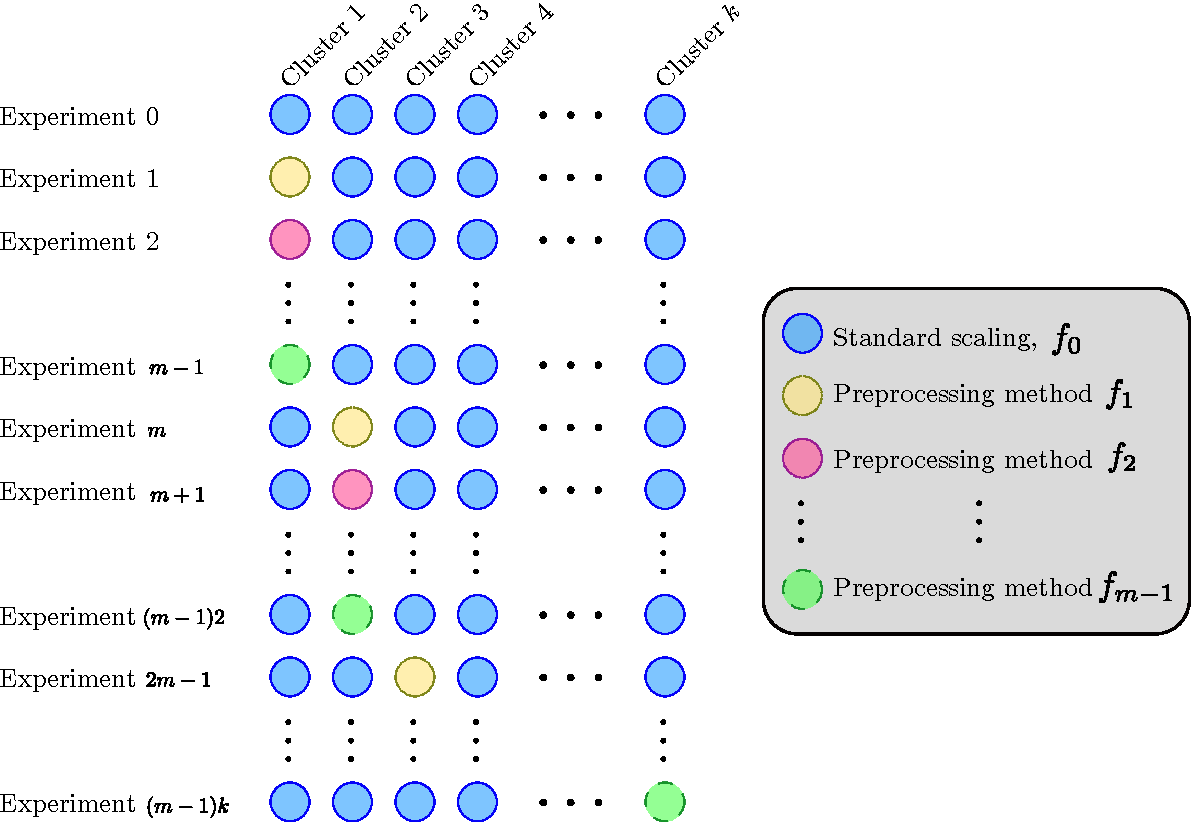
\includegraphics[width=\textwidth]{diagrams/prepmix-diagram.pdf}
    \end{center}
    \caption{Illustration of the ``ablation studies'' performed to determine
       the optimal preprocessing method
    for each cluster, as part of the \ac{PREPMIX-CAPS} routine.}
    \label{fig:prepmix}
\end{figure}

With the \ac{PREPMIX-CAPS} method, we want to transform the
data using the mixture of preprocessing techniques that gives the best
performance according to some validation metric. Usually, this is the
validation loss of the neural network being trained. As such, to determine
how effective some combination of the
$f_0, f_1,\dots,f_{m-1}$ preprocessing techniques are on the dataset,
we need train the model from scratch after transforming the training with
with our mixture. We will refer to this as one \textit{experiment}, and each experiment
gives us a value for the validation loss, which we interpret as the effectiveness
of the corresponding mixture of preprocessing techniques.
Recall that after clustering, we have $k$ clusters of variables and $m$ different
preprocessing methods to consider for each cluster. Trying all of the possible
combinations would require performing $m^k$ experiments, which is
computationally infeasible for large $k$ or $m$, especially if model training
is slow. Instead, we iteratively look at the isolated effect each of the
different preprocessing techniques have on a particular cluster, and repeat
this $k$ times, similar to an ablation study. This process is illustrated in
\cref{fig:prepmix}. For the clusters not being
considered in a particular experiment, a baseline preprocessing technique such
as standard scaling across time is applied to that cluster, as this technique in general
works well for most datasets \citep{preprocess_origin,nawi,singh}. This scheme reduces the number
of experiments from $m^k$ to $(m-1)k+1$, as we also do one experiment where the
baseline preprocessing technique is applied to all clusters. The scheme is
illustrated in \cref{fig:prepmix}, where we picked standard scaling as the
baseline preprocessing technique.

After these $(m-1)k+1$ experiments have been run, and the final validation loss has been recorded
for each experiment, we can analyse the results to determine what mixture of preprocessing
techniques to use. With \cref{fig:prepmix} as reference, let $\mathcal{L}_{C_{i},f_j}$
denote the validation loss associated with the experiment where
preprocessing method $f_j$, with $j>0$, was applied to cluster $C_i$.
For $C_1,\dots,C_k$, the validation loss
$\mathcal{L}_{C_i,f_0}$ is the validation loss from experiment 0, that is, the baseline experiment.
Then, the preprocessing method for cluster $C_i$ in the final mixture
is set to be $f_{\widehat{j}_i}$, where
\begin{equation}
    \widehat{j}_i=\argmin_{0 \leq j < m}  \mathcal{L}_{C_i,f_j}.
\end{equation}
Our approach to selecting the overall mixture based on separate marginal improvements in
performance makes the assumption
that the marginal improvements do not depend on how variables in a different cluster are
preprocessed.
This is a reasonable assumption to make.

\subsubsection{Optimisations}%
\label{ssub:Optimisations}

The different experiments, as shown in \cref{fig:prepmix}, have no dependencies
between them and can thus be executed in parallel. This allows speeding up the
experiment running phase through parallel computation.
Before starting the experiments, the set of \acp{GPU}
to use has to be configured, which we denote as $\mathcal{I}_{\textrm{device IDs}}$.
The number of jobs
to run concurrently on each \ac{GPU} at any point in time, denoted $n_{\textrm{num. jobs}}$, must
also be specified.
To allow parallel computation, all the experiments---or jobs---were encapsulated in a Python
\texttt{threading.Thread} object. The jobs were then allocated to the \acp{GPU} in
$\mathcal{I}_{\textrm{device IDs}}$ in a \textit{round-robin} fashion, that is, allocate the first
job to the first \ac{GPU}, the second job to the second \ac{GPU}, etc., wrapping around to the first
\ac{GPU} once we reach the last \ac{GPU}. This is done until up to
$\# \mathcal{I}_{\textrm{device IDs}} \cdot n_{\textrm{num. jobs}}$ have been allocated and
set to start executing.
When these jobs finish, subsequent experiments are scheduled in a similar
fashion. Unlike standard \textit{round-robin} scheduling, each job is run until completion instead
of switching while they execute.

% \subsection{Hyperparameters}%
% \label{sub:Hyperparameters}
%
% For my experiments, I used the following selection of preprocessing techniques:
% \begin{itemize}
%     \item Standard scaling \textit{with time- and dimension-axis}
%     \item Standard scaling \textit{across time}
%     \item Standard scaling followed by $\tanh(\cdot)$ \textit{with time- and dimension-axis}
%     \item Standard scaling followed by $\tanh(\cdot)$ \textit{across time}
%     \item Min-Max scaling to $[0,1]$ \textit{with time- and dimension-axis}
%     \item Min-Max scaling to $[0,1]$ \textit{across time}
% \end{itemize}
% This gives $m=6$. From hyperparameter tuning on $k$, also found $k=20$ for amex dataset
% (TODO: don't go into datasets yet...).
% For both clustering methods, the number of bins parameter, required for computing some of the
% statistics, as well as estimating the \ac{pdf} values required for estimating the
% \ac{KL-divergence} between the random variables, was set to be
% $n_{\textrm{num. bins}}=5000$. The number of clusters $k$ to use, was tuned using the specific
% dataset the \ac{PREPMIX-CAPS} method was applied to, which is described in section TODO.

% }}}

\section{Conclusion}% Conclusion
\label{sec:Conclusion}% {{{

We have now looked at three different novel preprocessing methods,
\ac{EDAIN}, \ac{EDAIN-KL}, and \ac{PREPMIX-CAPS}. The \ac{EDAIN} layer starts by applying
an adaptive outlier removal transformation, followed by an adaptive shift and scale operation,
and finally an adaptive power transform operation to reduce skewness. The layer also has
two modes, \textit{local-aware} and \textit{global-aware}, designed to handle highly
multimodal data and data with fewer modes, respectively. To optimise the parameters of
the \ac{EDAIN} layer, it is prepended to an existing neural network and the
\ac{EDAIN} parameters and neural network parameters are then simultaneously optimised using
stochastic gradient descent. We then looked at the \ac{EDAIN-KL} layer, which has the same
four sublayers as \ac{EDAIN}, but instead of optimising these using gradient descent, the layer
is treated as a bijector. Then it is optimized by minimizing the \ac{KL-divergence} between the
training data and a standard  normal distribution, transformed by the \ac{EDAIN-KL} layer.
After this, the training data is normalized by applying the inverse transformation.
The final method we looked at was the \ac{PREPMIX-CAPS} procedure, which is an automated
pipeline for selecting which static preprocessing technique to apply to each variable. It does this
by first clustering all the predictor variables. Then, through a parallel experiment
running phase, it selects the preprocessing method that minimizes the validation loss for each
cluster.

% }}}

%%%%%%%%%%%%%%%%%%%%%%%%%%%%%%%%%%%%%%%%%%%%%%%%%%
\chapter{Results} %%%%         Results        %%%%
%%%%%%%%%%%%%%%%%%%%%%%%%%%%%%%%%%%%%%%%%%%%%%%%%%
\label{ch:Results}

% Introduction
% Introduction {{{

In this chapter, we apply the methods proposed in \cref{ch:Methods} on both
synthetic data and two real-world datasets with very different characteristics.
The first real-world dataset contains
aggregated profile features of credit card customers at different statement
dates, and exhibits many traits commonly observed in
real-world datasets such as missing values, skewed distributions, and outliers
\citep{nawi,brits}.
The second dataset is based on a high-frequency stock market and
exhibits highly multi-modal distributions.
In our experiments, we give detailed descriptions of the
datasets used, describe the evaluation methodology, and specify the deep neural
networks used as well as describe how they are optimised and evaluated. In our
experiments, we also compare the performance of the proposed methods to
baseline static preprocessing methods, as well as other adaptive preprocessing
methods from the literature \citep{dain,bin}.

% }}}

%%%%%%%%%%%%%%%%%%%%%%%%%%%%%%%%%%%%%%%%%%%%%%%%%%%
\section{Simulation study}%%%  Simulation study   %%
\label{sec:Simulation study}%%%%%%%%%%%%%%%%%%%%%%%%%

% Introduction
% {{{
Before evaluating the different preprocessing methods proposed in \cref{ch:Methods} on real-world
data, we apply them on synthetic multivariate time-series data. This way, we can build
insight on how the different preprocessing methods transform the data and how effective the
transformations are, all in a controlled setup. As the different preprocessing techniques are
designed to handle irregularly-distributed data that might be skewed or contain outliers, just like
real-world data, we will synthesize data with such characteristics.
In this section, we first go through the novel data generation algorithm I propose, which
has several desirable properties for assessing the effectiveness of preprocessing
techniques. After this, we look at examples of how the distributions of the predictor variables
change when the dataset is transformed by the different preprocessing techniques. Then, we assess
their performance and discuss the results.

% TODO: add some benchmark times for how long it takes to generate samples?

% }}}

% Multivariate time-series data generation algorithm
\subsection{Multivariate time-series data generation algorithm}% {{{
\label{sub:data_gen}

The goal of the thesis is to design preprocessing methods that can increase performance,
ideally on a wide variety of irregular datasets.
As such, it will be very useful to have full control over how
the variables are distributed, ideally through only needing to specify an
unnormalized \ac{pdf} function for each variable.  Additionally, we
want the covariance structure of the generated data to resemble that of a
multivariate time-series. Lastly, as the time-series will be used in supervised
learning, we also want to generate a response $y \in \{0,1\}$ that is based on the
covariates. To my knowledge, there are no publicly-available
algorithms that meet all of these criteria, so I propose my own
data generation procedure that has all these properties.

We start by providing a general overview of the algorithm, then go more in-depth into
each part of it later.
The main input to the data generation procedure is the time-series length,
$T \in \mathbb{N}$, and the number of features, $d \in \mathbb{N}$.
For each predictor variable $j=1,2,\dots,d$,
we also specify an unnormalized \ac{pdf}, $f_j : \R \rightarrow {\R}^{+}$.
The  data generation procedure then generates a
multivariate time-series covariate $\bfX \in \R^{d\times T}$ and a corresponding response $y \in \{0,1\}$ in three steps,
each step providing one of the functional requirements we highlighted earlier. 
Note that this procedure is repeated $N$ times to, say, generate a
dataset of $N$ samples.
An overview of the the three steps of the data generation algorithm is shown in
\cref{eq:synth_algo1,eq:synth_algo2,eq:synth_algo3} below. Each row in the
three matrices corresponds to one predictor variable and the column specifies the timestep.
% Algorithm (equation diagram) TODO: add sample indices ^{(i)} to all the samples ?
% Also change all to lower-case to indiicate we are working with samples?
% Synth algo equation diagram {{{
\begin{align*}
    % Gaussian variable matrix left text
    \rotatebox[origin=c]{90}{{
            \parbox{3cm}{\textrm{Hidden correlated }\\
            \textrm{Gaussian RVs}}
    }}&\left\{
    \renewcommand\arraystretch{2}
    % Gaussian variable matrix
    \begin{matrix}
         N_{1,1} & N_{1,2} & \cdots & N_{1,T} \\
         N_{2,1} & N_{2,2} & \cdots & N_{2,T} \\
         \vdots & \vdots & \ddots & \vdots \\
         N_{d,1} & N_{d,2} & \cdots & N_{d,T}
    \end{matrix}\right.
    % Gaussian sample
    \;\sim\; \mathcal{N}(\mathbf{0}, \Sigma'), \textrm{ where } \Sigma' \in \R^{(dT) \times (dT)}%
    \addtocounter{equation}{1}\tag{\theequation}\label{eq:synth_algo1}
    \\%
     % Arrow down
     &\qquad\qquad\qquad\bigg\downarrow\quad U_{j,t}=\Phi_{\mathcal{N}}\left(
         N_{j,t} \big/\sqrt{\Sigma'_{jT+t,jT+t}}
     \right) \\
    % Uniform matrix text
    \rotatebox[origin=c]{90}{{
            \parbox{3cm}{\textrm{Hidden correlated }\\
            \textrm{uniform RVs}}
    }}&\left\{
    \renewcommand\arraystretch{2}
    % Uniform variable matrix
    \begin{matrix}
         U_{1,1} & U_{1,2} & \cdots & U_{1,T} \\
         U_{2,1} & U_{2,2} & \cdots & U_{2,T} \\
         \vdots & \vdots & \ddots & \vdots \\
         U_{d,1} & U_{d,2} & \cdots & U_{d,T}
    \end{matrix}\right.
    % Uniform form response
    \stackrel{\textrm{Form response}}{\xrightarrow{\hspace*{2cm} }}
    Y=\mathbb{I}\left(\sum^{d}_{j=1} \sum^{T}_{t=1} \beta_{j,t} U_{j,t}+\zeta > \frac{1}{2}  \right)
    \addtocounter{equation}{1}\tag{\theequation}\label{eq:synth_algo2} \\
     % Arrow down
     &\qquad\qquad\qquad\bigg\downarrow\quad X_{j,t}=\widehat{F^{-1}_j}\left(
         U_{j,t}
     \right) \qquad \forall t=1,2,\dots,T\\
    % Xs matrix text
    \rotatebox[origin=c]{90}{{
            \parbox{3.5cm}{\textrm{Output multivariate time-series}}
    }}&\left\{
    % Xs matrix
    \renewcommand\arraystretch{2}
     \begin{matrix}
         X_{1,1} & X_{1,2} & \cdots & X_{1,T} \\
         X_{2,1} & X_{2,2} & \cdots & X_{2,T} \\
         \vdots & \vdots & \ddots & \vdots \\
         X_{d,1} & X_{d,2} & \cdots & X_{d,T}
     \end{matrix}\right.
    \addtocounter{equation}{1}\tag{\theequation}\label{eq:synth_algo3}
\end{align*} 
% }}}

In the first step in \cref{eq:synth_algo1}, we generate Gaussian random variables that have
a similar covariance structure to a multivariate time-series. This ensures the covariates'
covariance more closely resemble that of real-world sequence data. In the second step, shown in
\cref{eq:synth_algo2}, we convert the Gaussian random variables into uniform random variables using
the inverse normal \ac{CDF}, after standardizing each variable.
In this step, we also form the response through a linear combination
of unknown parameters $\bm\beta$ and the uniform random variables. This ensures there is
some mutual information between the response and the covariates that are generated in the
final step.
In step 3, shown in \cref{eq:synth_algo3}, we form the final covariates using the provided
\acp{pdf} $f_1,f_2,\dots,f_d$. This is done by estimating each \ac{pdf}'s inverse \ac{CDF} using
numerical methods, and transforming the uniform random variables with these. This makes the samples
come from a distribution matching that of the provided \acp{pdf}.
We also note that the ``high-level covariance structure'' created in step 1 is maintained between
all the steps as the transformations are all monotonic, but the magnitudes might change somewhat.
Moreover, in \cref{eq:synth_algo1,eq:synth_algo2,eq:synth_algo3} we use random variable notation
for each of the steps, but in practice, all the transformations are applied on samples from these.

\subsubsection{Step 1: Generating random variables with a time-series covariance structure}%
\label{ssub:Step 1: Generating correlated random variables}

One approach to reproducing the covariance structure of a multivariate time-series is to assume
that each of the $d$ individual time-series follow a \textit{moving average} model, which is
a common type of theoretical time-series \citep{time-series}. With this model, the covariate at
timestep $t$ takes the form
\begin{equation}\label{eq:hs08da9sd}
    X_t=c-\sum^{q}_{j=0} \theta_j \epsilon_{t-j},
\end{equation}
where $c \in \R$ is a constant, $\epsilon_0,\epsilon_1,\dots$ are uncorrelated random variables with
zero mean and finite variance $\sigma_\epsilon\in\R$. Also, $\theta_0=-1$ and
$\theta_1,\dots,\theta_q \in (-1,1)$ are the unknown parameters.
Under this model, \cite{time-series} state that the covariance between a sample
from timestep $t$ and a sample from $\tau \in \mathbb{Z}$ timesteps into the
future is 
\begin{equation}\label{eq:osmmfoieie9}
    s_\tau=\textrm{cov}\{X_t,X_{t+\tau}\}=\sigma_\epsilon^2 \sum^{q-\tau}_{j=0}
    \theta_j \theta_{j+\tau}.
\end{equation}
We will not be generating our covariates using the model in \cref{eq:hs08da9sd} as this would
make it get samples that are distributed according to arbitrary \acp{pdf}. However,
we can use the covariance formula from \cref{eq:osmmfoieie9} to set the covariance between each
pair of variables generated. To do this, we first specify the parameters $q$, $\sigma_\epsilon$, and
$\theta_0,\dots,\theta_q$ for each of the $d$ predictor variables. Then, imagine stacking the
Gaussian random variables $N_{1,1}, N_{1,2}, \dots, N_{2,1}, N_{2,2}, \dots,
N_{d,T}$ in \cref{eq:synth_algo1} row-wise so that they form a $dT$-long vector. Let $\Sigma \in \R^{dT\times dT}$ denote the covariance matrix of this $dT$-long Gaussian multivariate random variable.
While still thinking of each $T$-length row as its own univariate time-series, fill out the 
entries in
$\Sigma$ based on \cref{eq:osmmfoieie9}, using the parameters specified for each of the $d$
time-series. The remaining entries of $\Sigma$ are randomly initialised with samples from
$\mathcal{N}(\mu=0,\sigma=\sigma_{\textrm{cor}})$, where
$\sigma_{\textrm{cor}}$ is a hyperparameter for the data synthesis, with the motivation being
to create some cross-dependence between each time-series.
In order to use $\Sigma$ as a valid covariance matrix for sampling from the
$dT$-dimensional
multivariate normal distribution, it needs to be
\textit{symmetric positive semi-definite}. The $\Sigma$ matrix we have constructed so far has no
guarantee of satisfying this. Therefore, we use the algorithm proposed by
\cite{nearest_psd} to find the symmetric positive semi-definite matrix
$\Sigma' \in \R^{dT \times dT}$ that is closest to $\Sigma$ according to the Frobenius norm.
More details on this procedure can be found in \cite{nearest_psd}.
After this, we generate a $dT$-dimensional sample $\mathbf{N} \sim
\mathcal{N}(\mathbf{0}, \Sigma')$ and imagine ``unrolling'' this into a
$d\times T$ matrix where we have a $T$-timestep-long time-series in each row,
just as in \cref{eq:synth_algo1}.

\subsubsection{Step 2: Forming the response}%
\label{ssub:Step 2: Forming the response}

Before forming the response $y$, we need to convert the Gaussian random variables generated in
step 1 into uniform random variables. It can be shown that if we divide a zero-mean normal random
variable by its standard deviation and pass it through its inverse \ac{CDF}-function, we obtain
a uniform random variable. Therefore, we do this for each of the normal random variables, as shown
in the transition between \cref{eq:synth_algo1} and \cref{eq:synth_algo2}, giving $d$ time-series
of uniform random variables, each of length $T$.

To form the response, we randomly sample a noise term $\zeta \sim \mathcal{N}(0,\sigma_\zeta^2)$
and set
\begin{equation}
    Y=\mathbb{I}\left(\sum^{d}_{j=1} \sum^{T}_{t=1} \beta_{j,t} U_{j,t}+\zeta > \frac{1}{2}  \right).
\end{equation}
The idea behind this is to make sure each variable contributes to the response, but the contribution
of each variable might differ and some might be completely irrelevant, just like in real-world
data.
Note that the noise term $\zeta$ 
is regenerated for each multivariate time-series $\bfX \in \R^{d \times T}$
we generate, while the
parameters $\bm\beta \in \R^{d \times T}$ are held fixed for each time-series generated
as part of a synthetic dataset.
When synthesizing a new dataset of say $N$ samples, we first generate \textit{one set} of
$\bm\beta \in \R^{d \times T}$ unknown parameters with
$\beta_{1,1},\dots,\beta_{d,T} \stackrel{\textsc{iid}}{\sim} \mathcal{N}\left(\frac{1}{dT},\sigma_{\beta}^2\right)$, where
$\sigma_\beta$ is another hyperparameter for the dataset synthesis. The mean $\frac{1}{dT}$
was set to
ensure the dataset generated is balanced, that is, the ratio between true and false labels is equal.
To show this, we first note that
\begin{align}
    \mathbb{E}\left(
        \sum^{d}_{j=1} \sum^{T}_{t=1} \beta_{j,t} U_{j,t}+\zeta
    \right)
    &=\sum^{d}_{j=1} \sum^{T}_{t=1}  \mathbb{E}\left(\beta_{j,t} U_{j,t} \right)+0 \nonumber\\
    &=\sum^{d}_{j=1} \sum^{T}_{t=1}  \mathbb{E}\left(\beta_{j,t}\right)
    \mathbb{E}\left(U_{j,t} \right), \textrm{ as } U_{j,t}, \beta_{j,t}\textrm{ are uncorrelated}\nonumber \\
    &=\sum^{d}_{j=1} \sum^{T}_{t=1} \frac{1}{dT} \frac{1}{2} =\frac{1}{2} \label{eq:s9sad}.
\end{align}
As the variables $\beta_{j,t}$s, $U_{j,t}$ and $\zeta$ are all symmetrically distributed, it can
be shown that the term inside the $\mathbb{E}(\cdot)$ is also symmetric, so it follows from
\cref{eq:s9sad} that $\mathbb{E}(Y)=\mathbb{P}(Y=1)=\frac{1}{2}$. This makes the class distribution in the
synthesized dataset balanced, which is a nice property to have.

\subsubsection{Step 3: Transforming the variables based on provided PDFs}%
\label{ssub:Step 3: Estimating the inverse CDF}

The third step of the data generation procedure involves taking samples from
uniformly distributed random variables $U_{j,t} \sim \textrm{U}[0,1]$ and transforming them
using the inverse \ac{CDF} of the corresponding specified \ac{pdf}, $f_j$, which results in
a sample from the distribution specified by $f_j$. To do this, we need to estimate the inverse
\ac{CDF} function $\widehat{F^{-1}_j}(\cdot)$ using only $f_j$. This is done by evaluating
$f_j$ on a fine-grid of values $\mathcal{X}=\{A_j,A_j+\delta,A_j+2\delta,\dots,B_j\}$, where
$A_j$, $B_j$, and $\delta$ are additional
hyperparameters specified in conjunction with the \ac{pdf} $f_j$.
Then we use \textit{trapezoidal numerical integration}, of which \cite{num_anal} provide
a reference for, to estimate
$\widehat{F_j}(x)=\int_{-\infty}^x f_j(x') dx'$  for all $x \in \mathcal{X}$. Since the provided
\acp{pdf} are unnormalized, we normalize the \ac{CDF} estimates by dividing them by
$\widehat{F_j}(B_j)$.
To get $\widehat{F_j^{-1}}(\cdot)$, we create an inverse \textit{look-up table} that maps the
$\widehat{F_j}(x)$-values to the corresponding $x$-values. When implementing this procedure,
the look-up table is \textit{cached} to ensure the integration only needs to be done
once for each $x \in \mathcal{X}$. Then, to evaluate $\widehat{F^{-1}_j}(u)$ for some $u \in (0,1)$,
we perform a \textit{binary search} on the look-up table to find the smallest $x \in \mathcal{X}$ such that
$\widehat{F_j}(x) \geq u$, which can efficiently be done since the values are already in sorted order
because \acp{CDF} are monotonically increasing. A reference for binary search is given by
\cite{algorithms_go_brrr}.


% }}}

% Preprocessing method experiments
\subsection{Preprocessing method experiments}% {{{
\label{sub:synth_data_exp_results}

We now use the data generation procedure described in \cref{sub:data_gen} to synthesize some
multivariate time-series data in order to assess the different preprocessing methods proposed
in \cref{ch:Methods}. We also use this synthetic data to illustrate how the different methods
transform the data distribution.
% Explaining the pdfs
To effectively asses how well the different preprocessing method work, and
to stretch them to their limits, we want to design variable distributions that are
highly irregular and infeasible for a simple linear transformation, like
standard scaling, to undo. We also note that these distributions are based on real-world
data like the Amex dataset and the FI-2010 LOB dataset, as we will see in
\cref{sec:amex_data} and \cref{sec:lob_data}.
We consider the following, possibly unnormalized, \acp{pdf}:
\begin{align}
    f_1(x)&= 10 \cdot\Phi_{\mathcal{N}}\left(10\left\{x+4\right\}\right)\cdot p_{\textrm{N}}(x+4)
    +  \mathbb{I}(8 < x < 9.5) \frac{e^{x-8}}{10}, \label{eq:synth_pdf1}\\
    f_2(x)&= \left\{
        \renewcommand\arraystretch{2}
        \begin{matrix*}[l]
            20 \cdot p_{\mathcal{N}}(x-20), & \textrm{ if } x > \pi; \\
            e^{x/6}\cdot\left(10\sin(x)+10 \right), & \textrm{ if } x \leq \pi,
        \end{matrix*}
    \right. \label{eq:synth_pdf2}\\
        f_3(x)&=
        2 \cdot \Phi_{\mathcal{N}}\left(-4 \{ x-4\}\right) \cdot p_{\mathcal{N}}(x-4), \label{eq:synth_pdf3}
\end{align}
where $p_{\mathcal{N}}(\cdot)$ and $\Phi_{\mathcal{N}}(\cdot)$ denotes the \ac{pdf}
and \ac{CDF} of the standard normal distribution, respectively.
Qualitatively, the first variable has a skewed normal distribution centred at $x=-4$ with some
outliers in the range $8 < x < 9.5$. The second variable has a multimodal distribution with
exponentially decaying mode heights as $x$ decreases, and there is a Gaussian mode
at $x=20$. The third variable is simply a skewed normal distribution centred at
$x=4$ with shape parameter $\alpha=-4$. Samples generated from the three distributions are
visualised in the first row of \cref{fig:synth_examples}.

% Experiment setup paragraph
For our synthetic data experiment, I synthesized $N_\mathcal{D}=100$ datasets, each with
$N=50\;000$ multivariate time-series of length $T=10$ and  $d=3$ predictor variables at each
timestep $t=1,2,\dots,T$. The predictor variables were configured to be distributed according to
the \acp{pdf} specified in \cref{eq:synth_pdf1,eq:synth_pdf2,eq:synth_pdf3}. Note that due to
an efficient implementation of the data generation procedure described in
\cref{sub:data_gen}, generating all this data took less than 10 seconds.
For each of the $N_{\mathcal{D}}$ datasets, we perform a 80\%-20\% train-test split and train
a new \ac{GRU} \ac{RNN} model on the training data after
using one of our preprocessing techniques to transform the whole dataset. The trained model
was then evaluated using the remaining 20\% of the data, that is, the validation data.
The loss, the binary classification accuracy, and the Amex metric, which is described
in \cref{sec:amex_meth}, were used to evaluate each preprocessing method.
The full details of the hyperparameters used for all these experiments can be found in
\cref{ch:synth_data_appendix}. This was repeated for standard scaling, the \ac{BIN} method
proposed by \cite{bin}, the \ac{DAIN} method proposed by \cite{dain}, the \ac{EDAIN-KL} method,
the local-aware \ac{EDAIN} method and the global-aware \ac{EDAIN} method, all proposed by me.
Additionally, we evaluate the model on unprocessed raw data and using a gold standard which I will
refer to as ``\ac{CDF} inversion''. This gold standard method assumes we have perfect information about the
data generation procedure, which means we know both $f_1,f_2,f_3$ and hence can
estimate their \acp{CDF} $\widehat{F_1},\widehat{F_2},\widehat{F_3}$.
This means we can transform the samples from $X_{j,t}$ using the transformation
\begin{equation}
    \tilde{x}_{j,t}=\Phi_{\mathcal{N}}^{-1}\left(\widehat{F_j}(x_{j,t})\right),
\end{equation}
which gives $\tilde{X}_{j,t} \sim \mathcal{N}(0,1)$. This data is a lot easier for the \ac{RNN} model
to handle compared to the irregularly-distributed samples from the unprocessed data.
In the last row of \cref{fig:synth_examples}, we can see how this method works in practice,
noting that it is able to perfectly transform each predictor variable such that the resulting
distribution is standard normal.

% Example transformation figure
% figure {{{
\begin{figure}
    \begin{center}
        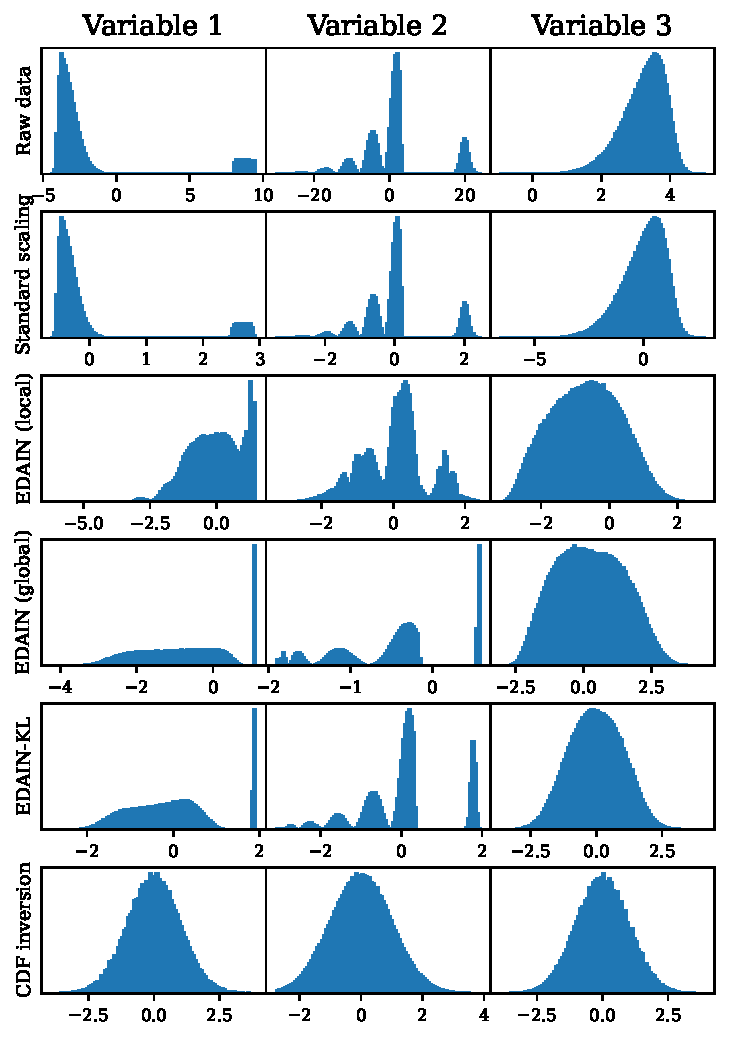
\includegraphics[scale=1]{figures/synthetic_data_example_transformations.pdf}
    \end{center}
    \caption{%
        Examples of applying the different preprocessing methods on the $d=3$ different
        predictor variables from the synthesized multivariate time-series dataset.
        In each plot, we consider the data points
        $\mathcal{X}=\left\{x^{(i)}_{j,t}\right\}_{i=1,2,\dots,N,t=1,2,\dots,T}$ where
        $j \in \{1,2,3\}$ is specified by the column title.
        Additionally, the data points are only from the first of the
        $N_{\mathcal{D}}=100$ different dataset, and the preprocessing models are those that were
        fit on this dataset.
    }
    \label{fig:synth_examples}
\end{figure}
% }}}

% Discussing example transformation paragraph
We now look more closely at how each of the proposed methods transform data in a visual manner.
Consider \cref{fig:synth_examples}, where I have plotted the unprocessed data along with the same
data transformed by each of the trained preprocessing models. We first
notice how standard scaling is not able to handle this data well as even the transformed data still
has many irregularities like significant outliers. Considering the local-aware \ac{EDAIN} method
next, we see how it is able to condition the transformation on the mode each sample from variable
2 came from. This allows it to push all the modes closer together in order to get closer to a
standardized Gaussian distribution, but we note that the result is still multimodal.
Likewise, the local-aware method was also able to merge the two modes seen in variable 1.
Turning our attention to the global-aware \ac{EDAIN} method, we see how it is able to utilise
the power transform and outlier removal sublayers to reduce the skewness and push the outlier
samples closer to the main distribution, respectively. The former is especially noticeable in
variable 3. The \ac{EDAIN-KL} method works similarly, but is able to reduce the skewness seen
in variable 3 to a greater extent since its optimisation objective is the normality of each
variable, not a low classification loss. Yet, this method has the highest performance
metric values after the gold-standard method and global-aware \ac{EDAIN}.
As discussed earlier, the \ac{CDF} inversion method is able to perfectly normalize each variable
because it assumes full knowledge of the data generation mechanism.

% Synthetic data experiment table
% Table {{{
\begin{table}[htp]
    \centering
    \begin{tabular}{l|ccc}
        \toprule
        Method        & Validation loss &     Validation Amex metric &            Validation ACC\% \\
        \midrule
        Unprocessed data   & $0.1900 \pm 0.0362$           & $0.8268 \pm 0.0359$          & $91.68 \pm 1.68$           \\
        Standard scaling   & $0.1873 \pm 0.0108$           & $0.8306 \pm 0.0136$          & $91.73 \pm 0.65$          \\
        \ac{CDF} inversion & $\mathbf{ 0.1627 \pm 0.0094}$ & $\mathbf{0.8504 \pm 0.0123}$          & $\mathbf{92.89 \pm 0.55}$ \\
        BIN                & $0.2191 \pm 0.0103$           & $0.8009 \pm 0.0120$          & $90.36 \pm 0.59$          \\
        DAIN               & $0.2153 \pm 0.0146$           & $0.8077 \pm 0.0152$          & $90.48 \pm 0.78$          \\
        EDAIN (local)      & $0.2099 \pm 0.0095$           & $0.8110 \pm 0.0109$          & $90.71 \pm 0.57$          \\
        EDAIN (global)     & $\mathbf{0.1636 \pm 0.0086}$           & $\mathbf{0.8506 \pm 0.0110}$ & $\mathbf{92.83 \pm 0.51}$          \\
        EDAIN-KL           & $0.1760 \pm 0.0094$           & $0.8402 \pm 0.0111$          & $92.24 \pm 0.59$          \\
        \bottomrule
    \end{tabular}%
    \caption{
        Evaluation results using the synthesized datasets. Lower loss, 
        higher Amex metric, and higher ACC\% is better. All confidence intervals are 95\% asymptotic
        normal based on $N_{\mathcal{D}}=100$ different metric values for
        each method. The ACC\% is the prediction accuracy, where the predicted class is the
        class with the highest assigned probability in the output of the model.
        The two best-performing methods have been highlighted in bold.
    }%
    \label{tab:synth_results}
\end{table}
% }}}

% Discussing experiment results table
For each of the preprocessing methods considered, we also recorded performance metrics for each
of the $N_{\mathcal{D}}=100$ times we trained it with an \ac{RNN} model on a new dataset.
The results are
shown in \cref{tab:synth_results}. We first notice how the performance metrics are more unstable
if the data is not preprocessed, as evident from the high variance. Second, we see how the
performance can be improved a lot by applying a suitable preprocessing method instead of just
using the unprocessed data. Moreover, we notice that the preprocessing of the data is
not limited to always applying standard scaling, as for instance the global-aware \ac{EDAIN} method
gives a significantly lower validation loss at significance level $\alpha=5\%$, when
compared to standard scaling. In fact, standard scaling barely improves on the unprocessed data,
likely due to irregularity of the data and the fact that a non-linear transformation is required
to normalize the variables.  This is a great motivation for the research conducted on more advanced
preprocessing methods in this thesis.

Another key takeaway from \cref{tab:synth_results} is that sequence
models such as \acp{RNN} handle normally-distributed data a lot better than irregularly-distributed
data. This is evident from how the \ac{CDF} inversion case gives the best performance, with the
transformed data being samples from a standard Gaussian distribution. This further motivates this
thesis' research on coming up with sophisticated preprocessing methods to normalize irregular data.
Since the \ac{CDF} inversion gives the best performance and it assumes perfect information of the
data generation mechanism, we can think of it as the ``gold standard'' in this experiment.
Yet, the global-aware \ac{EDAIN} method achieves very similar performance as their
average performance metric values only differ at the third or fourth decimal point. This highlights
how well the global-aware \ac{EDAIN} method is able to learn what sort of transformation
is most suitable to apply to the data in order to improve performance as much as possible.
Lastly, we note that three local-aware normalization methods, \ac{BIN},
\ac{DAIN} and local-aware \ac{EDAIN}, all perform worse than when the data is unprocessed.
This is likely due to them not being monotonic like the rest of the methods,
which hurts performance in this case due to the response being generated from a
linear combination of the hidden uniform random variables.

% }}}

%%%%%%%%%%%%%%%%%%%%%%%%%%%%%%%%%%%%%%%%%%%%%%%%%%%%%%%%%%%%%%%%%%%%%%%%
\section{American Express default prediction dataset}%%%  Amex dataset %%%
\label{sec:amex_data}%%%%%%%%%%%%%%%%%%%%%%%%%%%%%%%%%%%%%%%%%%%%%%%%%%%%%%

% Introduction
% {{{
The first real-world dataset we will test our proposed processing methods on is
the default prediction dataset published by \cite{amex-data} on behalf of
American Express.  This dataset was first used in a Kaggle%
\footnote{\url{https://www.kaggle.com/}} competition, where data scientists
competed online for three months to produce the model with the highest predictive performance
on the dataset
\citep{amex-data}.  For the rest of the thesis, I will refer to the dataset as
the \textit{Amex dataset}.

This section is structured as follows. We first describe the
dataset in more detail and give the motivation for why it was selected for the study of
preprocessing methods. Then, we present the initial data preprocessing performed to allow it to
be used for our experiments. After this, we
cover the  methodology used when evaluating the different preprocessing methods on
the dataset, including details on the deep sequence model used, how it was optimised, and
the metrics used for evaluating its performance.
We also list the hyperparameters selected for the different preprocessing methods.
Finally, we present the experimentation results and look at how well each of the proposed methods
perform on the Amex dataset. While doing this, we also compare their performance to state of
the art methods and a baseline preprocessing technique.
% }}}

% Description
\subsection{Description}% {{{
\label{sub:Description}

The Amex dataset contains data from $N=458\,913$ customers. For each customer
$i=1,2,\dots,N$, a vector of $d=188$ aggregated profile features has been
recorded at $T=13$ different credit card statement dates, producing a multivariate
time-series on the form $\bfX^{(i)}\in \R^{d \times T}$. Given this, the task is to predict
the binary label $y^{(i)} \in \{0,1\}$ indicating whether customer $i$
defaulted or not, that is, whether they were able to pay back their credit card
balance amount within 120 days after their latest credit card statement date
\citep{amex-data}. This is done by creating a model that takes input
$\bfX^{(i)} \in \R^{d \times T}$ and outputs the probability of a default
event, that is $\mathbb{P}(Y^{(i)}=1)$.  In the dataset provided by
\cite{amex-data}, the non-default records have been \textit{down-sampled} such
that the final default rate in the dataset is about 25\%.  Additionally, the
feature names have all been anonymized, but they can be categorised into the
five categories: delinquency variables, spend variables, payment variables,
balance variables, and risk variables \citep{amex-data}.  Additionally, 11 of
the 188 features are categorical, so only the 177 numerical features will be
considered for preprocessing in this thesis.

% EDA plot
% figure {{{
\begin{figure}
\begin{center}
    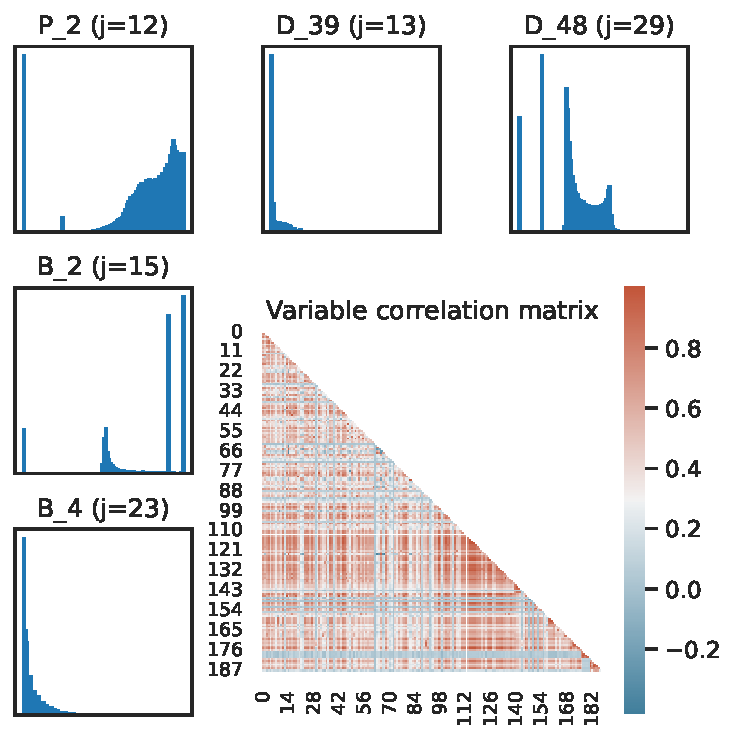
\includegraphics[scale=1]{figures/amex_data_eda_plot.pdf}
\end{center}
\caption{
    \ac{EDA} plot for the American Express default prediction
    dataset.  The bottom-right plot show a correlation matrix between each pair
    of the $d=188$ predictor variables. All correlations are computed using
    Pearson's correlation coefficient, $\rho$, and the colour indicates the
    value of the coefficient.  The other five plots show histograms of five
    different predictor variables with $n_{\textrm{bins}}=100$,
    chosen to give a representative overview of
    how the different variables in the dataset are distributed.
    % Note on why axes dropped
    Note that both the $x$- and $y$-axes have been dropped because the histograms
    are meant to give an idea of the ``shape'' of the distributions, and 
    the scale and exact density values are not needed to convey this.
}
\label{fig:amex_eda}
\end{figure}

% }}}

% talk about motivation, why stuiable for preprocessing research, refer to EDA
% plots etc.
The Amex dataset is very suitable for research on preprocessing techniques for
deep learning. As we see in \cref{fig:amex_eda}, the dataset exhibits many traits commonly observed in
real-world datasets, such as skewed distributions, multiple modes, unusual
peaks, and extreme values \citep{nawi}. 
Recalling the synthesized irregular distributions visualised in \cref{fig:synth_examples},
the distributions in the Amex dataset show similar traits. For example, the
P\_2 variable in\ \cref{fig:amex_eda} looks like a mirrored version of the first variable in the
synthetic dataset. We also see a case of multiple modes in the D\_48 variable, which we
also synthesized. Even though the synthesized data contains highly irregularly-distributed data,
it is not too far away from what we might observe in real-world datasets, as examplified
by \cref{fig:amex_eda}.
The Amex dataset also has a lot of missing values, also common in
real-world dataset \citep{nawi, brits}. Moreover, most of the predictor variables are heavily
correlated, as seen in \cref{fig:amex_eda}.
As such, if the proposed preprocessing methods
work well on this dataset, they are likely to perform well to other real-world datasets as well.

% }}}

% Initial data preprocessing
\subsection{Initial data preprocessing}% {{{
\label{sub:Data formatting}

For privacy reasons, before the data was published by \cite{amex-data}, it was min-max
normalized to the range $[0, 1]$. Then a random noise term $\bm\epsilon \sim
\textrm{U}[-0.01,+0.01]$ was added to each variable for each sample.
For more accurate experimentation, I tried to undo this process. This was
done by first de-noising the dataset, and then undoing the min-max normalization by selecting
a random scale and shift for each variable. More details on the exact procedure can be found
in  \cref{ch:undo_amex_pre}.

The raw dataset contains many missing values, with some variables having up to 90\% missing
values.  Across the whole dataset, 8.50\% of the numeric data points are
missing. Five variables also have more than 91\% of their data points missing,
and only 138 out of the 177 numeric variables have less than 1\% missing
values. How to best handle missing values is its own active research area in deep learning
\citep{weerakody2023,brits}, and this project does not focus on that.  Instead, we
focus on preprocessing techniques applied to a dataset where the missing values
have already been treated. However, our neural network cannot process input
data that is not fully numeric, so we will need to fill in the missing values.
Dropping the time-series with missing values is also not an option
since every single time-series has at least one missing value. We choose the simplest
option of handling missing values, that is, replacing them with a constant.
Since the data is normalized to fall in the range
$[0,1]$, I chose to fill all the missing values with the value $-0.5$, to avoid
camouflaging the missing values among the non-missing ones.
For the categorical entries, the missing values are replaced with -1.

In addition to missing values, some customers also have fewer than 13 credit
statements recorded. This makes some time-series shorter than others in the
dataset, which is problematic for the preprocessing techniques that are applied
with the time- and dimension-axis.  Additionally, it makes batching the data
cumbersome. Therefore, the shorter time-series are \textit{padded} with numeric
constants such that they are all of length $T=13$. For this, I chose to pad the
numeric values with -1 and the categorical values with -2, to distinguish between
padded values and missing values.

% }}}

% Evaluation methodology
\subsection{Evaluation methodology}% {{{
\label{sec:amex_meth}

Before looking at the preprocessing experiment results on the Amex dataset in \cref{sub:amex_res},
we first describe how the experiments are conducted, including the choice of sequence model,
and a description of how it is trained and evaluated. In each experiment, we split the training data into five
20\% splits. We then train and evaluate the model using 5-fold cross-validation, which works
as follows: If relevant, we fit the preprocessing method on the 80\% training data split and use
it to transform all of the data. The sequence model is the trained using the 80\% training data
split, and its predictions on the unseen  20\%  split are used for computing validation losses
and evaluation metrics.
This is repeated for each of the five splits, giving us five different validation losses and
evaluation metric values.
This subsection is structured as follows:
We first present the architecture of the deep sequence model used for predicting the probability of
a default event for each customer. We then move onto describing the hyperparameters associated with
optimising this model, including choices such as the loss function and the optimizer. Then we
go over the evaluation metrics used for this particular dataset, which are computed on the 20\%
validation splits as described earlier.


\subsubsection{Sequence model}%
\label{ssub:Sequence model}

We chose to use a relatively simple \ac{RNN} sequence model, with a classifier head, as our
baseline model.
It consists of two stacked \ac{GRU} \ac{RNN} cells, both with a hidden dimensionality of 128.
Between these cells, there is a dropout layer with the dropout probability set to $p_{\textrm{drop}}=20\%$.
Dropout is a technique used during training where each neuron is randomly deactivated with
probability $p_{\textrm{drop}}$, which helps increase generalization performance \citep{dropout}.
We also have 11 categorical features. These are
passed through seperate embedding layers, each with a dimensionality of 4. The outputs of the
embedding layers and the numeric columns, after passing them through the two \ac{GRU} units,
are then combined and passed to the classifier head. The classifier head is a conventional
linear neural network consisting of 2 linear layers with
128 and 64 units each, respectively, and separated by a \ac{ReLU} activation function.
The output is then fed through
a linear layer with a single output neuron, followed by a sigmoid activation function to constrain
the output to be a probability in the range $(0,1)$. This allows feeding the model with
a multivariate time-series $\bfX^{(i)} \in \R^{d \times T}$ and get a probability
$p_i \in (0,1)$ as the output, which we interpret as the probability of a default event.
The details on how we arrived at the hyperparameters for the model architecture can be found in \cref{sec:hyp_amex_mod}.

\subsubsection{Optimising the model}%
\label{ssub:Optimising the model}

Since the targets are binary labels $y_1,y_2,\dots,y_N \in \{0,1\}$ and our predictions are
probabilities $p_1,p_2,\dots,p_N \in (0,1)$, a suitable loss function is binary cross entropy loss.
This gives the criterion
\begin{equation}
    \mathcal{L}(p_i,y_i)=- \left\{y_i \log p_i + (1-y_i) \log\left( 1- p_i \right)\right\}.
\end{equation}
After preprocessing the data according to whatever preprocessing method we are evaluating,
the data is fed
in batches to the \ac{GRU} \ac{RNN} model and its unknown parameters are optimised according
to the description in \cref{sec:Deep learning}. This is done using a batch size of 1024 and
a base learning rate of $\eta=10^{-3}$. The optimizer used was the Adam optimizer proposed by
\cite{adam}, with the momentum parameters set to $\beta_1=0.9$ and $\beta_2=0.999$.
Model training efficiency and convergence speed can be improved by selecting a suitable learning
rate during model training, which is easier with dynamic learning rates selected by a learning
rate scheduler \citep{lr_demyst}. Therefore, we use a multi-step learning rate scheduler with milestones
at 4 and 7 epochs, and a stepsize of $\gamma=0.1$. This means that the learning rate for epochs
1 to 3 is $\eta$, from 4 to 6 is $\gamma\eta$ and from epoch 7 and beyond is $\gamma^2\eta$.
The maximum number of epochs was set to 40, but we also used an early stopper on the validation loss
with a patience of 5 epochs, so training could terminate earlier.
The details on how all of these hyperparameters were selected can be found in \cref{sec:hyp_amex_opt}.

\subsubsection{Evaluation metrics}%
\label{ssub:Evaluation metrics}

%%% The metric used %%%
For evaluating the performance on the Amex dataset, we will consider the binary cross-entropy loss
computed on the 20\% validation split, referred as the \textit{validation loss}. Additionally,
we will use a metric referred to as the \textit{Amex metric }, proposed for use on this dataset
by \cite{amex-data}. The Amex metric is 50\%-50\% weighted split between the
normalized Gini coefficient, $G$ and the default rate captured at 4\%, denoted $D$
\citep{amex-data}.

Assume we have made predictions $p_1,p_2,\dots,p_N$ for each of the $N$ customers, and assume these
predicted default probabilities have been sorted in non-increasing order. Also assume they have
associated normalized weights $w_1,w_2,\dots,w_N$ such that $\sum_{i=1}^N w_i=1$.
To compute $D$, we take the predictions $p_1,p_2,\dots,p_\omega$
captured within the highest-ranked 4\% of our predictions considering the
weights $w_1,w_2,\dots,w_N$. Then, we look at the default rate within these predictions, normalized
by the overall default rate. In other words,
\begin{equation}
    D= \frac{\sum^{\omega}_{i=1} y_i}{\sum^{N}_{i=1} y_i},
    \textrm{ where } \omega \textrm{ is the highest integer such that }
    \sum^{\omega}_{i=1} w_i \leq 0.04. %\cdot\sum^{N}_{i=1} w_i.
\end{equation}

We now describe how to compute $G$, which requires computing the Gini coefficient in two ways for
$k \in \{0,1\}$.
From \cite{gini}, we know the Gini coefficient can be computed as
\begin{equation}\label{eq:fdjf09j}
    G_k=2  \sum^{N}_{j=1} w_{i^{(k)}_j} \left(\frac{p_{i^{(k)}_j} - \overline{p}}{\overline{p}}\right)
    \left(\hat{F}_{i^{(k)}_j} - \overline{F} \right),
\end{equation}
where $\hat{F}_{i^{(k)}_j}={w_{i^{(k)}_j}}\big/{2} +\sum^{j+1}_{\ell=1}
w_{i^{(k)}_\ell}$ and $\overline{p}=\sum^{N}_{j=1} w_{i^{(0)}_j}
p_{i^{(0)}_j}=\sum^{N}_{j=1} w_{i^{(1)}_j} p_{i^{(1)}_j}$
and $\overline{F}=\sum^{N}_{j=1} w_{i^{(0)}_j}
\hat{F}_{i^{(0)}_j}=\sum^{N}_{j=1} w_{i^{(1)}_j} \hat{F}_{i^{(1)}_j} $.
To compute the normalized Gini coefficient, we first sort the predictions in non-decreasing order
by the \textit{true labels} $y_1,y_2,\dots,y_N$, and denote this ordering $i^{(0)}_1, i^{(0)}_2, \dots, i^{(0)}_N$.  Let $G_0$ denote the result of computing \cref{eq:fdjf09j} with this sorting.
Then we sort the values by the \textit{predicted probabilities} $p_1,p_2,\dots,p_N$ in non-decreasing order, denoting this ordering as $i^{(1)}_1, i^{(1)}_2, \dots, i^{(1)}_N$.
Let the value of \cref{eq:fdjf09j} computed with this ordering be denoted $G_1$.
The normalized Gini coefficient is then $G=G_1/G_0$, which is what we use in the final metric
\begin{equation}
    \textrm{Amex metric}=\frac{1}{2} \left(G +D \right)= \frac{1}{2} \left(\frac{G_1}{G_0}  +D \right).
\end{equation}

% }}}

% Preprocessing method experiments
\subsection{Preprocessing method experiments}% {{{
\label{sub:amex_res}

We now look at the performance of
the three novel methods that were proposed in \cref{sec:EDAIN-method,sec:EDAIN-KL-method,sec:PREPMIX-CAPS-method}, that is, the \ac{EDAIN} method, the \ac{EDAIN-KL} method, and the \ac{PREPMIX-CAPS} method.
All these methods were compared to the state of the art within research on adaptive preprocessing
methods for multivariate time-series data, which includes the \ac{DAIN} method proposed
by \cite{dain} and the
\ac{BIN} method proposed by \cite{bin}. Additionally, as a baseline method, we also compare the
aforementioned methods to standard scaling applied across time, as this is a commonly used
preprocessing method \citep{singh,nawi,stanislav}.
Before providing an overview of the results found, we briefly go over the
hyperparameters chosen for each of the preprocessing methods tested.

\subsubsection{Hyperparameters}%
\label{ssub:Learning rate tuning}

As described in \cref{sub:edain_opt_sgd}, when optimising the adaptive preprocessing methods
through stochastic gradient descent, we should select individual learning rates for each part
of the adaptive preprocessing layer, lest the convergence might be unstable.
As the \ac{DAIN} and \ac{BIN} layer has never been applied to the Amex dataset, we need
to tune these learning rates ourselves. The details of how I performed this tuning is found in
\cref{sec:hyp_amex_prep}.

% Move onto specific mentions of learning rates for the different layers
For the DAIN layer, the optimal learning rate parameter for the shift layer
and scale layer were found to be $\eta_{\textrm{shift}}=\eta_{\textrm{scale}}=1.0$. Recall that
the actual learning rate is this parameter multiplied by the base learning rate $\eta$.
Despite the \ac{DAIN} layer consisting of three sublayers: an adaptive shift layer, an adaptive
scale layer, and an adaptive gating layer, the adaptive gating layer is not used in my
experiments because \cite{dain} found its inclusion to decrease
performance when used together with an \ac{RNN} sequence model, likely due to the \ac{GRU}
\ac{RNN} model having its own gating mechanism.
For the \ac{BIN} layer, the optimal learning rate modifiers for the different parameters were
found to be $\eta_\beta=10.0$, $\eta_\gamma=1.0$ and $\eta_\lambda=10^{-6}$.
For the \ac{EDAIN} layer, the optimal learning rate modifiers were found to be
$\eta_{\textrm{scale}}=10^{-2}$, $\eta_{\textrm{shift}}=10^{-2}$, $\eta_{\textrm{outlier}}=10^{2}$,
and $\eta_{\textrm{power}}=10$. Additionally, for this method, we only consider the global-aware
mode as the local-aware mode was designed to handle more multimodal datasets, of which the Amex
dataset is not. The local-aware \ac{EDAIN} method is thus not expected to outperform the global-aware
version on the Amex dataset.

% Tuning for EDAIN-KL and PREPMIX-CAPS
The \ac{PREPMIX-CAPS} and \ac{EDAIN-KL} layers also have hyperparameters that need
tuning. With the \ac{PREPMIX-CAPS} routine, we need to select $k$. The optimal $k \in \mathbb{N}$
was found to be $k=20$, and the detail of how this was found is in \cref{sec:hyp_amex_prep}.
Additionally, the statistics-based clustering method was used instead of the \ac{KL-divergence}-based
method, and the linkage criteria was set to \textit{average}. Additionally, the number of bins
was set to be $n_{b}=5000$. For the \ac{EDAIN-KL} layer, the optimal learning
rate modifiers were found to be
$\eta_{\textrm{scale}}=10$, $\eta_{\textrm{shift}}=10$, $\eta_{\textrm{outlier}}=10^{2}$,
and $\eta_{\textrm{power}}=10^{-7}$.


\subsubsection{Overview of results}%
\label{ssub:amex-results}

% Amex convergence plot (a) loss (b) AMEX metric
% multi-figure {{{
\begin{figure}[htp]
    \centering
    \begin{subfigure}[b]{0.99\textwidth}
        \centering
        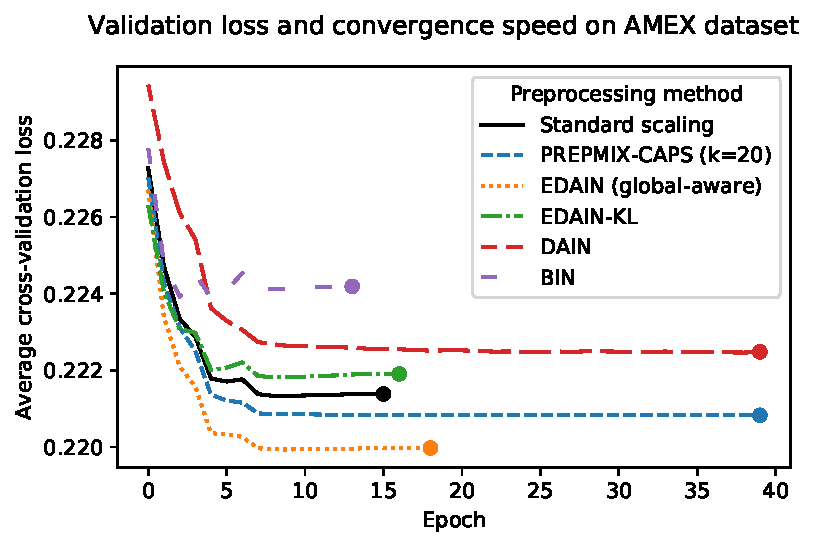
\includegraphics[scale=.9]{figures/amex_performance_convergence.pdf}
        \caption{Average cross-validation loss of \ac{RNN} model after each training epoch.
        Lower is better.}
        \label{fig:amex_performance_loss}
    \end{subfigure}
    \hfill
    \begin{subfigure}[b]{0.99\textwidth}
        \centering
        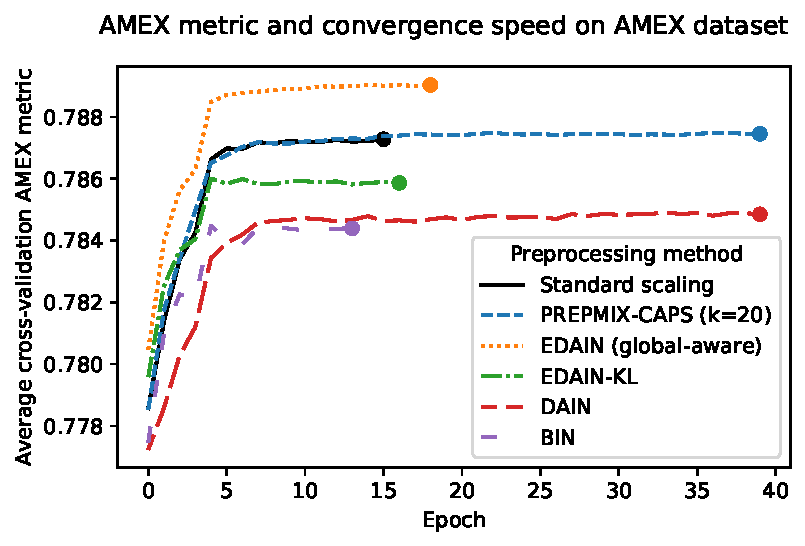
\includegraphics[scale=.9]{figures/amex_performance_convergence_metric.pdf}
        \caption{Average cross-validation American Express competition metric of the \ac{RNN} model
        after each training epoch. Higher is better.}
        \label{fig:amex_performance_metric}
    \end{subfigure}
    \caption{
        The plots show the average cross-validation performance of different preprocessing methods
        applied to the American Express dataset when training a \ac{RNN} binary classification model.
        The cross-validation was done using five disjoint 20\% validation sets.
        The dot highlights the earliest epoch where all five models are deemed to have converged by
        the early stopper, and can be interpreted as the convergence speed. A dot further left is
        better.
    }%
    \label{fig:amex_performance}
\end{figure}
% }}}

% Amex performance table
% table {{{
\begin{table}[htp]
    \centering
    \begin{tabular}{lcc}
        \toprule
        Method & Validation loss & Amex metric \\
        \midrule
        Standard scaling & $0.2213 \pm 0.0039$ & $0.7872 \pm 0.0068$ \\
        PREPMIX-CAPS (k=20) & $0.2208 \pm 0.0033$ & $0.7875 \pm 0.0053$ \\
        EDAIN (global-aware) & $\mathbf{0.2199} \bm\pm \mathbf{0.0034}$ & $\mathbf{0.7890} \bm\pm \mathbf{0.0078}$ \\
        EDAIN-KL & $0.2218 \pm 0.0040$ & $0.7858 \pm 0.0060$ \\
        DAIN & $0.2224 \pm 0.0035$ & $0.7847 \pm 0.0054$ \\
        BIN & $0.2237 \pm 0.0038$ & $0.7829 \pm 0.0064$ \\
        \bottomrule
    \end{tabular}%
    \caption{
        Evaluation results using the American Express default prediction dataset. Lower validation
        loss and higher Amex metric is better.
        All confidence intervals are based on evaluation metrics from 5 cross-validation folds,
        and are asymptotic normal 95\% confidence intervals.
        The experiment methodology, including a description of the metrics,
        is given in  \cref{sec:amex_meth}.
    }%
    \label{tab:amex_performance}%
\end{table}
% }}}

% Amex fold breakdown
% TODO: augment with plot of the metric folds as well!
% figure {{{
\begin{figure}[htp]
    \begin{center}
        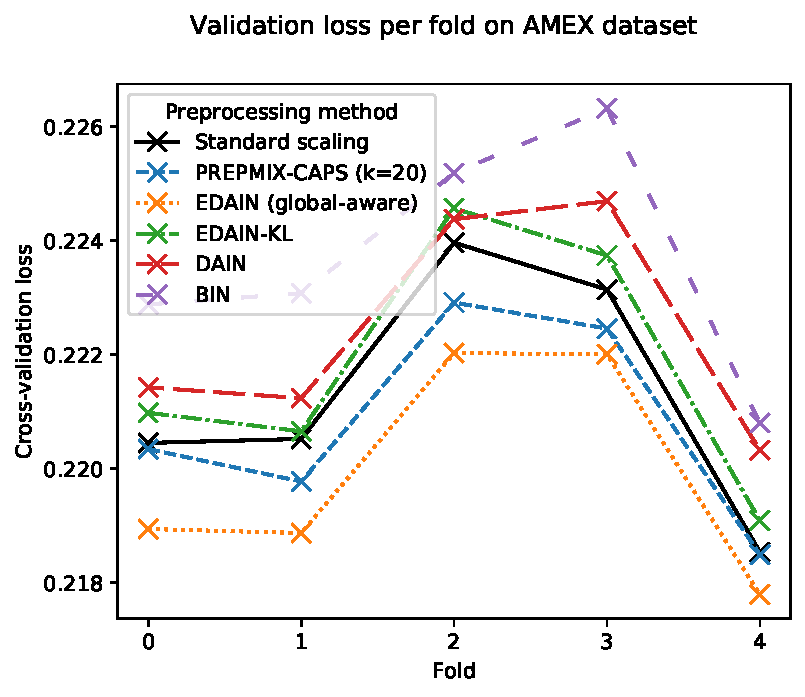
\includegraphics[scale=0.9]{figures/amex_performance_convergence_per_fold}
    \end{center}
    \caption{
        Validation loss at convergence for each of the five folds in the American Express
        default prediction dataset. Lower is better.
    }%
    \label{fig:amex_folds}
\end{figure}
% }}}

In \cref{fig:amex_performance}, we see the average validation loss and Amex metric for the
5-fold cross-validation experiments using the different preprocessing methods. From the plots,
we see that the global-aware \ac{EDAIN} outperforms all the other methods tested, both
when looking at the average validation loss and when looking at the average Amex metric value.
However, it is slightly slower to convergence when compared to standard scaling,
\ac{EDAIN-KL} and \ac{BIN}, but only by a few epochs.
% The subfigures:
% In \cref{fig:amex_performance_loss} and \cref{fig:amex_performance_metric},
In \cref{tab:amex_performance}, we present a confidence interval for the validation loss and Amex
metric, based on the 5 different folds. For both
the Amex metric and validation loss,
these 95\% confidence intervals overlap for all the methods. As such, from this table
alone, we cannot conclude that the proposed global-aware \ac{EDAIN} is significantly better than
the other methods. However, most of the variance comes from the folds themselves. Consider the
validation loss shown for each of the 5 folds in \cref{fig:amex_folds}. Here, we see that despite
the validation loss varying from fold-to-fold, the global-aware \ac{EDAIN} method beats the
competition on all folds. From this plot, we can also rank the methods with \ac{EDAIN} as the
best performing, \ac{PREPMIX-CAPS} in second place, and standard scaling in third place.
The performance difference between \ac{EDAIN-KL} and \ac{DAIN} is then somewhat overlapping,
but \ac{BIN} performs the worst out of the methods tested on the Amex dataset.
Looking at the average validation loss and Amex metric in \cref{tab:amex_performance}, we notice
that all the methods, even standard scaling, improves upon \ac{DAIN} and \ac{BIN}, even though
the latter methods are recent, novel preprocessing methods. A possible explanation for this
observation is presented later in \cref{sub:local_vs_global}.

% TODO: also integrate comments from Francesco on the results plot in this section!

% }}}

%%%%%%%%%%%%%%%%%%%%%%%%%%%%%%%%%%%%%%%%%%%%%%%%%%%%%%%%%%%%%
\section{FI-2010 Limit order book dataset}%%%  LOB dataset %%%
\label{sec:lob_data}%%%%%%%%%%%%%%%%%%%%%%%%%%%%%%%%%%%%%%%%%%%

% Introduction
% {{{

The second real-world dataset we apply the proposed preprocessing techniques to
is a publicly available%
\footnote{\url{https://etsin.fairdata.fi/dataset/73eb48d7-4dbc-4a10-a52a-da745b47a649}},
large-scale dataset called FI-2010, which contains several \ac{LOB} records from
a high-frequency stock market \citep{lob-data}.
Due to the differing characteristics between the stocks in this market, this dataset is a lot
more multi-modal compared to the Amex dataset. In \cref{fig:lob_eda}, we see the distribution of
some of the predictor variables. Notice how it is highly multi-modal and resembles the
second predictor variable synthesized in \cref{fig:synth_examples}.
We start this section off by providing a more detailed description of the \ac{LOB} dataset,
as well as some relevant terminology. Then we go through the methodology used for evaluating
the preprocessing techniques, including descriptions of the sequence model  architecture,
how it is optimised, and what evaluation metrics we use. Lastly, we look at the performance
of the proposed local-aware and global-aware \ac{EDAIN}  method and the proposed \ac{EDAIN-KL}
method, and compare it to the state of the art \ac{DAIN} and \ac{BIN} methods proposed
by \cite{dain} and \cite{bin}, respectively.

% }}}

% Description
\subsection{Description and terminology}% {{{
\label{sub:Description}

% EDA plot
% figure {{{
\begin{figure}
    \begin{center}
        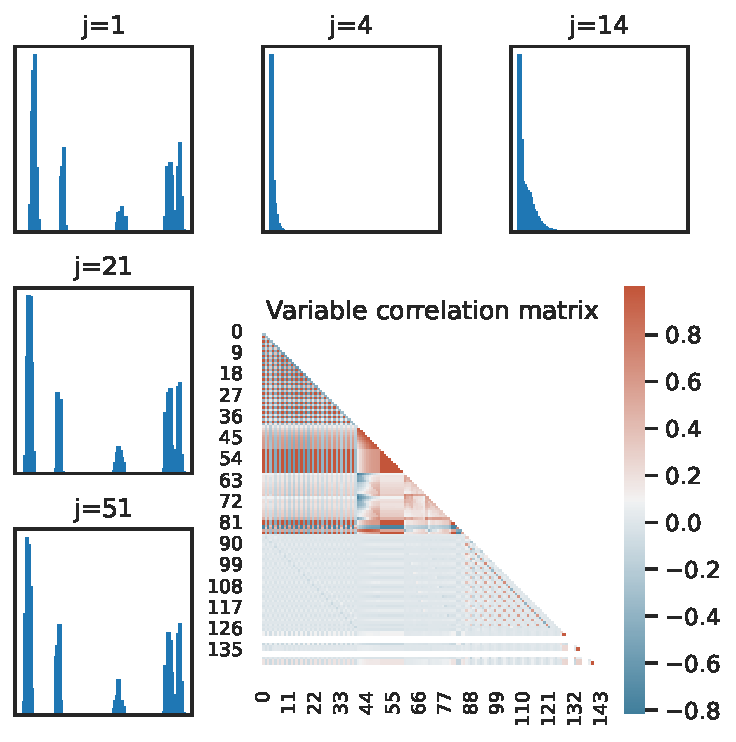
\includegraphics[scale=1]{figures/lob_data_eda_plot.pdf}
    \end{center}
    \caption{
        \ac{EDA} plot for the FI-2010 \ac{LOB} dataset.
        The bottom-right plot show a correlation matrix between each pair
        of the $d=144$ predictor variables. All correlations are computed using
        Pearson's correlation coefficient, $\rho$, and the colour indicates the
        value of the coefficient.  The other five plots show histograms of five
        different predictor variables, chosen to give a representative overview of
        how the different variables in the dataset are distributed.
        % Note on axes dropped
        Note that both the $x$- and $y$-axes have been dropped because the histograms
        are meant to give an idea of the ``shape'' of the distributions, and 
        the scale and exact density values are not needed to convey this.
    }
    \label{fig:lob_eda}
\end{figure}

% }}}

We start by explaining some of the terminology related to the FI-2010 \ac{LOB} dataset.
A limit order is an order to buy or sell an asset or stock with a restriction on the maximum
or minimum price, respectively.
There are two types of limit orders: A bid order indicates the highest price at
which someone is willing to buy an asset, while an ask order is the lowest
price at which someone is willing to sell their asset \citep{gould2013limit}.
The FI-2010 dataset contains \acp{LOB}, that is,
records of limit orders, gathered from a high-frequency stock market.
The data was collected over 10 business days in June 2010
from five Finnish companies \citep{lob-data}. Note
that only the ten lowest and ten highest ask and bid order prices were recorded.
The data from \cite{lob-data} was cleaned and features were extracted based on the pipeline
proposed by \cite{lob_preprocess}, of which \cite{dain} has made publicly available%
\footnote{The preprocessed FI-2010 dataset can be found here: \url{https://github.com/passalis/dain}}.
%
This resulted in $N=453\,975$ vectors of dimensionality $d=144$, which can all be ordered by their
timestamp.
To use this data efficiently, we slide across the vectors using a window of
$T=15$ timesteps.
The task is then to predict whether the \textit{mid price} will increase, decrease or remain
stationary $H$ timesteps after the end of the current window. That is, given a multivariate
time-series $\bfX^{(i)} \in \R^{d \times T}$ with $d=144$ and $T=15$, predict whether the
mid price will decrease, remain stationary or increase $H=10$ timesteps into the future.
The integer $H$ is called the
\textit{horizon}, and to follow suite with the experiments conducted by \cite{dain},
we use the horizon $H=10$.
The mid price is the average of the highest bid price and the lowest ask price. We label a stock
as stationary if the mid price changes by less than 0.01\% within the horizon of $H=10$ timesteps.


% }}}

% Evaluation methodology
\subsection{Evaluation methodology}% {{{
\label{sec:lob_meth}

In this subsection, we describe the methodological approach to evaluating the proposed
preprocessing methods on the FI-2010 \ac{LOB} dataset.
Like with the Amex dataset, we split our
data into several folds, fit the preprocessing techniques and sequence model on the training
data, and evaluate the fit using various evaluation metrics on the corresponding validation split.
However, the splitting of the dataset, the model and loss function used, and the evaluation metrics
considered differ from our experiments on the Amex dataset. Therefore, in this subsection, we first
describe how we perform cross-validation on \ac{LOB} dataset. Then we describe the sequence
model used. After this, we describe the loss function and optimizer used to fit the sequence
model. Finally, we consider the evaluation metrics.

\subsubsection{Cross-validation}%
\label{ssub:Cross-validation}

We use the \textit{anchored cross-validation scheme}  proposed by \cite{lob-data}.
This means we use the first day of data to train the model, then evaluate it on the second
day of data. Afterwards, the first two days of data is used for training, and the third day
for evaluation. This is repeated until we use the first 9 days of data and the 10th day for evaluation. This scheme is illustrated in \cref{fig:lob_anchor}.
In total, we evaluate the model and preprocessing methods on 9 different folds.

% This figure was produced by running
%     pdfcrop --margins '0 0 0 -377' lob_paper_p12.pdf lob_cross_val_diagram.pdf
% on a PDF copy of the 12th page of the LOB FI-2010 paper
\begin{figure}
\begin{center}
    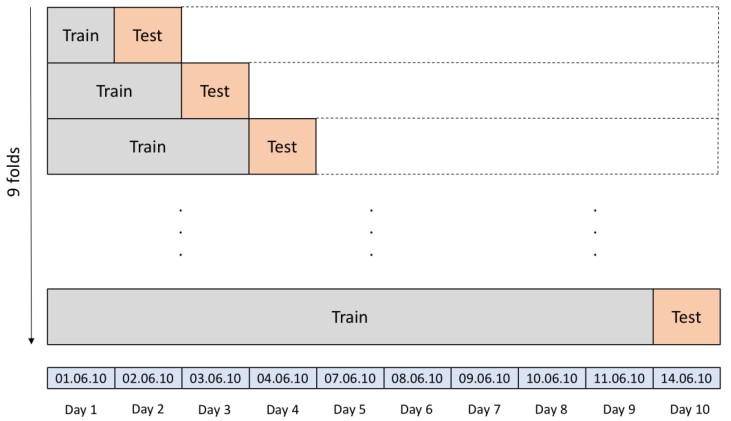
\includegraphics[width=\textwidth]{diagrams/lob_cross_val_diagram.pdf}
\end{center}
\caption{Anchored cross-validation experimental setup framework. This diagram is taken from
page 12 of \cite{lob-data}.}
\label{fig:lob_anchor}
\end{figure}

\subsubsection{Sequence model}%
\label{ssub:Sequencemodel2}

For the FI-2010 \ac{LOB} dataset, we use
a similar \ac{GRU} \ac{RNN} model as with the Amex dataset, but change the architecture slightly
to match the \ac{RNN}
model used by \cite{dain} in their paper. This was done to make the comparison between the
proposed \ac{EDAIN} method and their \ac{DAIN} method more fair, seeing as they also used the
\ac{LOB} dataset to evaluate \ac{DAIN}.
We now describe the model architecture.
Instead of using two stacked \ac{GRU} cells as described in
\cref{ssub:Sequence model}, we just have one with 256 units.
We also do not need any embedding layers because all the predictor variables are numeric, that is,
there are no categorical variables.
The classifier head that follows the \ac{GRU} cells then consists of one linear
layer with 512 units, followed by a \ac{ReLU} layer and a dropout layer with dropout probability
set to $p_{\textrm{drop}}=0.5$.  The output layer is
a linear layer with 3 units, as we are classifying the multivariate time-series into one of
three classes, $\mathcal{C}=\{\textrm{decrease}, \textrm{stationary}, \textrm{increase}\}$.
These outputs are then passed to a \textit{softmax} activation function such that the
output is a probability distribution over the three classes and sums to 1.
The softmax activation function is defined as
\begin{equation}
    \left[\textrm{softmax}(\bfy)\right]_j=\frac{e^{y_j}}{\sum^{k}_{i=1} e^{y_i}} ,\qquad j=1,2,\dots,k.
\end{equation}
In our case, we have $k=3$.

\subsubsection{Optimising the model}%
\label{ssub:as8dhasdh}

Recall that the targets are ternary labels $y_1,y_2,\dots,y_N \in \{0,1,2\}$, denoting whether the mid-price
decreased, remained stationary, or increased. The output of the model is, as discussed above,
probability vectors $\mathbf{p}_1, \mathbf{p}_2,\dots, \mathbf{p}_N \in
(0,1)^3$. Therefore, a suitable loss function is the cross-entropy loss
function, defined as
\begin{equation}
    \mathcal{L}(\mathbf{p}_i, y_i)=-\sum^{2}_{c=0} \mathbb{I}\{y_i=c\} \log \left( p_{i,c} \right),
\end{equation}
where $p_{i,c}$ denotes the predicted probability of class $c$ for the $i$th input sample.
For example, we interpret $p_{42,0}$ as the predicted probability that the mid price will decrease
based on 42$^{\textrm{nd}}$ multivariate time-series sample.
The \ac{GRU} \ac{RNN} model was then trained according to the description in
\cref{sec:Deep learning}. This was done using a batch size of 128. The optimizer used
was the RMSProp optimizer proposed by \cite{rmsprop}. The base learning rate was set to
$\eta=10^{-4}$. No learning rate scheduler nor early stoppers were used%
\footnote{%
    Despite not using any early stoppers,
    all the metrics were computed based on the model state at the epoch where the validation loss
    was lowest. This was because
    the generalization performance started to decline in the middle of training in most cases.
}.
This was done to best reproduce the methodology used by \cite{dain}.
At each training fold, the model was trained for 20
epochs. The details on how all these hyperparameters were selected can be found in
\cref{sec:hyp_lob_opt} and \cref{sec:hyp_lob_prep}.

\subsubsection{Evaluation metrics}%
\label{ssub:Evaluation metrics}

For evaluating the model performance on the FI-2010 \ac{LOB} dataset, we look at the
macro-$F_1$ score and Cohen's $\kappa$ metric.
Recall that we have three classes for our true labels,
$\mathcal{C}=\{\textrm{decrease}, \textrm{stationary}, \textrm{increase}\}$.
We consider the predicted label to be the entry with the highest probability in the
probability vector $\mathbf{p}_i \in (0,1)^3$, which is the output of the model.
Then, let $\textrm{TP}_c$, $\textrm{FP}_c$, $\textrm{TN}_c$
and $\textrm{FN}_c$ denote the true-positive, false-positive, true-negative and
false-negative rates for each class $c \in \mathcal{C}$. We then have that the precision and
recall for class $c \in \mathcal{C}$ is defined as
\begin{equation}
    \textrm{precision}_c= \frac{\textrm{TP}_c}{\textrm{TP}_c+\textrm{FP}_c}
    \qquad \textrm{recall}_c=\frac{\textrm{TP}_c}{\textrm{TP}_c+\textrm{FN}_c}.
\end{equation}
The $F_1$ score for a single class $c \in \mathcal{C}$ is then
\begin{equation}
    F_1^{(c)}=2\frac{\textrm{precision}_c  \cdot \textrm{recall}_c}{\textrm{precision}_c+\textrm{recall}_c} .
\end{equation}
The \textit{macro-}$F_1$ score metric is then simply the arithmetic mean of the $F_1$ score for
the different classes, that is
\begin{equation}
    \textrm{macro-}F_1=\frac{1}{|\mathcal{C}|}  \sum^{}_{c \in \mathcal{C}}  F_1^{(c)}.
\end{equation}

The second metric we consider is Cohen's $\kappa$ metric, which is computed as
\begin{equation}
    \kappa=\frac{p_o-p_e}{1-p_e} \in [-1,+1],
\end{equation}
where $p_o$ is the \textit{observed} probability of agreement between the true label and the
predicted label, and $p_e$ denotes the \textit{expected} agreement between the true and predicted
labels, assuming they are independently resampled from a distribution matching the empirical
distribution of the true labels and predicted labels, respectively \citep{kappa}.
Thus, this metric measures the level of agreement between the predicted and true labels,
accounting for agreement by chance. Perfect agreement is indicated by $\kappa=1$, and a value of
$\kappa=0$ indicates that there is no agreement between the predictions and the true labels,
other than what would be expected by chance \citep{kappa}.

% }}}

% Preprocessing method experiments
\subsection{Preprocessing method experiments}% {{{
\label{sub:Preprocessing method experiments}

For the preprocessing method experiments on the FI-2010 \ac{LOB} dataset, we look at the
performance of the proposed \ac{EDAIN} method, including both its local-aware and global-aware
mode, and the proposed \ac{EDAIN-KL} method. The performance of the proposed methods
are compared to the state of the art in
adaptive preprocessing techniques for multivariate time-series, those being
\ac{DAIN} and \ac{BIN}, both of which have already been evaluated on the \ac{LOB}
dataset by \cite{dain} and \cite{bin}, respectively. We also make comparisons to baseline
preprocessing methods such as standard scaling and min-max scaling. However, before looking
at all of these results, we briefly go over the hyperparameters selected for each of the
adaptive preprocessing methods tested.

\subsubsection{Learning rate hyperparameters}%
\label{ssub:Learning rate tuning}

As with the Amex dataset, we should also tune the individual learning rates of the sublayers in
all the adaptive preprocessing methods, otherwise convergence might be unstable.
Both \ac{DAIN} and \ac{BIN} have been applied to the \ac{LOB} dataset, but only \ac{DAIN} has been
used with an identical \ac{RNN} architecture as what we use in this thesis \citep{dain}. Therefore, the
optimal learning rate modifiers found by \cite{dain} for the \ac{DAIN} layer will be used
in our testing, those being $\eta_{\textrm{shift}}=10^{-2}$ and $\eta_{\textrm{scale}}=10^{-8}$.
For the \ac{EDAIN} and  \ac{BIN} methods, a grid search was performed to find the optimal learning
rates. This gave $\eta_\beta=1$, $\eta_\gamma=10^{-8}$, and $\eta_\lambda=10^{-1}$ for \ac{BIN},
$\eta_{\textrm{scale}}=\eta_{\textrm{shift}}=10$, $\eta_{\textrm{out}}=10^{-6}$ and $\eta_{\textrm{pow}}=10^{-3}$ for
global-aware \ac{EDAIN}, and
$\eta_{\textrm{scale}}=10^{-4}$, $\eta_{\textrm{shift}}=10^{-2}$, $\eta_{\textrm{out}}=10$ and $\eta_{\textrm{pow}}=10^{-1}$ for
local-ware \ac{EDAIN}.
More details on the procedure for determining these modifiers can be found in \cref{sec:hyp_lob_prep}.

\subsubsection{Overview of results}%
\label{ssub:Overview of results}

% LOB performance table
% table {{{
\begin{table}[htp]
    \centering
    \begin{tabular}{lcc}
        \toprule
        Method & Cohen's Kappa, $\kappa$ & Macro $F_1$-score \\
        \midrule
        Standard scaling & $0.2772 \pm 0.0550$ & $0.5047 \pm 0.0403$ \\
        Min-max scaling & $0.2618 \pm 0.0783$ & $0.4914 \pm 0.0603$ \\
        BIN & $0.3670 \pm 0.0640$ & $0.5889 \pm 0.0479$ \\
        DAIN & $0.3588 \pm 0.0506$ & $0.5776 \pm 0.0341$ \\
        EDAIN (local-aware) & $\bm{0.3836 \pm 0.0554}$ & $\bm{0.5946 \pm 0.0431}$ \\
        EDAIN (global-aware) & $0.2820 \pm 0.0706$ & $0.5111 \pm 0.0648$ \\
        EDAIN-KL & $0.2870 \pm 0.0642$ & $0.5104 \pm 0.0519$ \\
        \bottomrule
    \end{tabular}%
    \caption{
        Evaluation results using the FI-2010 limit order book dataset.
        Higher $\kappa$ and higher macro-$F_1$-score is better.
        All confidence intervals are based on evaluation metrics from 9 cross-validation folds,
        and are asymptotic normal 95\% confidence intervals.
        The experiment methodology, including a description of the metrics,
        is given in  \cref{sec:lob_meth}.
    }%
    \label{tab:lob_performance}%
\end{table}
% }}}

% LOB cross-validation breakdown
% figure {{{
\begin{figure}[htp]
\begin{center}
    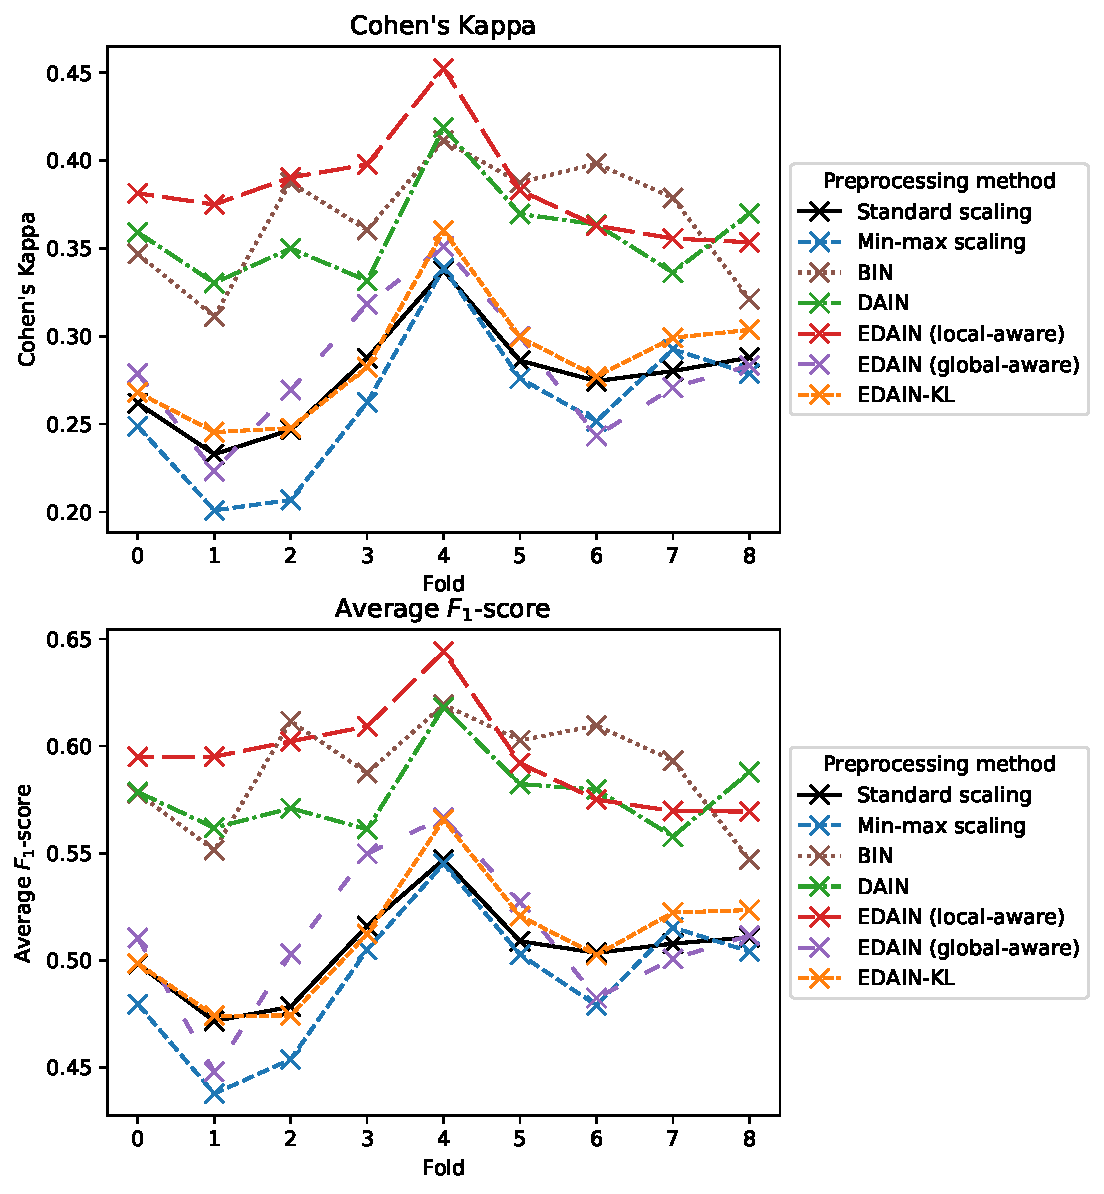
\includegraphics[width=\textwidth]{figures/lob_performance_per_fold.pdf}
\end{center}
\caption{
    Validation $\kappa$ and macro-$F_1$-value at convergence for each of the
    nine folds in the FI-2010 limit order book dataset.
    Higher $\kappa$ and higher $F_1$-score is better.
    The experiment methodology, including a description of the metrics,
    is given in  \cref{sec:lob_meth}.
}
\label{fig:lob_folds}
\end{figure}
% }}}

In \cref{tab:lob_performance}, we see the average macro-$F_1$ score and Cohen's $\kappa$ metric
for the nine different validation folds, along with a 95\% confidence interval for each metric.
For both metrics, the different preprocessing methods' performance fall into two groups.
The first group consists of standard scaling, min-max scaling, global-aware \ac{EDAIN} and
\ac{EDAIN-KL}, all of which achieve similar performance with average $\kappa$ metric values
in the range 0.26-0.29 and macro-$F_1$ values around 0.49-0.51. The second group of methods,
 \ac{BIN}, \ac{DAIN} and local-aware \ac{EDAIN}, all perform noticeably better than the
first group, with average $\kappa$ values in the range 0.36-0.38 and mean macro-$F_1$ scores around
0.58-0.59. This is likely because all the methods in the second group do
\textit{local-aware normalization} where the shift and scale depends on summary statistics computed
for each sample. None of the methods in the first group do this. This phenomenon will be
discussed further  in \cref{sub:local_vs_global}.
% Mention how EDAIN ga and EDAIN-KL still better than ss
Within the first group, we notice that global-aware \ac{EDAIN} and \ac{EDAIN-KL} both slightly
outperform standard scaling. This is also somewhat evident in \cref{fig:lob_folds}, where
especially \ac{EDAIN-KL} beats standard scaling on most of the folds.
% Mention that EDAIN la still slightly better than BIN and DAIN
In the second group, the mean $\kappa$ metric and mean macro-$F_1$ score are higher for the
proposed local-aware \ac{EDAIN} method when compared to the existing \ac{BIN} and \ac{DAIN}
methods. However, when considering the per-fold performance in \cref{fig:lob_folds}, there are some
folds where either \ac{BIN} or \ac{DAIN} outperform the proposed local-aware \ac{EDAIN} method.

% }}}

\section{Conclusion}%
\label{sec:Conclusion} % Conclusion {{{

In this chapter, the preprocessing methods proposed in \cref{ch:Methods} were applied to
both synthetic and real-world data, and we found that the proposed \ac{EDAIN} method outperformed
all the other methods on both the synthetic dataset and the Amex dataset, and in most cases on the
\ac{LOB} dataset.
After describing the proposed synthetic data generation algorithm, we generated
several multivariate time-series datasets with highly-irregular distributions. In our
\ac{EDA} of the Amex dataset, and \ac{LOB} dataset, we also saw how such irregular distributions
are present in real-world data as well.
Before presenting the experimental results on both the real-world datasets, we covered
the deep neural network architectures used and the evaluation methodology applied.
On both the synthetic dataset and the Amex dataset, we found the global-aware \ac{EDAIN} method
to clearly outperform both standard scaling and recent methods from the literature, with
\ac{EDAIN} almost being as good as our gold standard in the former case.
The \ac{PREPMIX-CAPS} procedure and \ac{EDAIN-KL} also showed promising results, ranking second on the Amex dataset and the synthetic dataset, respectively, if we exclude the gold-standard.
On the \ac{LOB} dataset, which was more multi-modal in nature, the local-aware normalization
methods showed had clearly higher performance. Here, the proposed local-aware \ac{EDAIN} method showed
the best performance, but its ranking relative to the \ac{DAIN} and \ac{BIN} methods from recent
literature was not as clear-cut as on the other two datasets.

% }}}

%%%%%%%%%%%%%%%%%%%%%%%%%%%%%%%%%%%%%%%%%%%%%%%%%%%
\chapter{Discussion} %%%%    Discussion        %%%%
%%%%%%%%%%%%%%%%%%%%%%%%%%%%%%%%%%%%%%%%%%%%%%%%%%%
\label{ch:Discussion}

% Introduction
% Introduction {{{

We start our discussion with the \ac{EDAIN} method, comparing its local-aware mode
with the other local-aware preprocessing methods, such as
\ac{DAIN} and \ac{BIN}, and compare its global-aware mode with \ac{EDAIN-KL}.
In doing so, we provide some
interesting insight on how the ``local-awareness'' or ``global-awareness'' of a preprocessing method
affects its performance on the two datasets, and illustrate this difference with plots. We then move onto discussing the \ac{EDAIN-KL} method and highlight some of its key advantages
that sets it apart from some of the other preprocessing methods discussed in this thesis. Finally,
we discuss the \ac{PREPMIX-CAPS} routine briefly. For all the preprocessing methods proposed,
we also provide a detailed discussion on their limitations.

% }}}

% Examples figure
% figure {{{
\begin{figure}
\begin{center}
    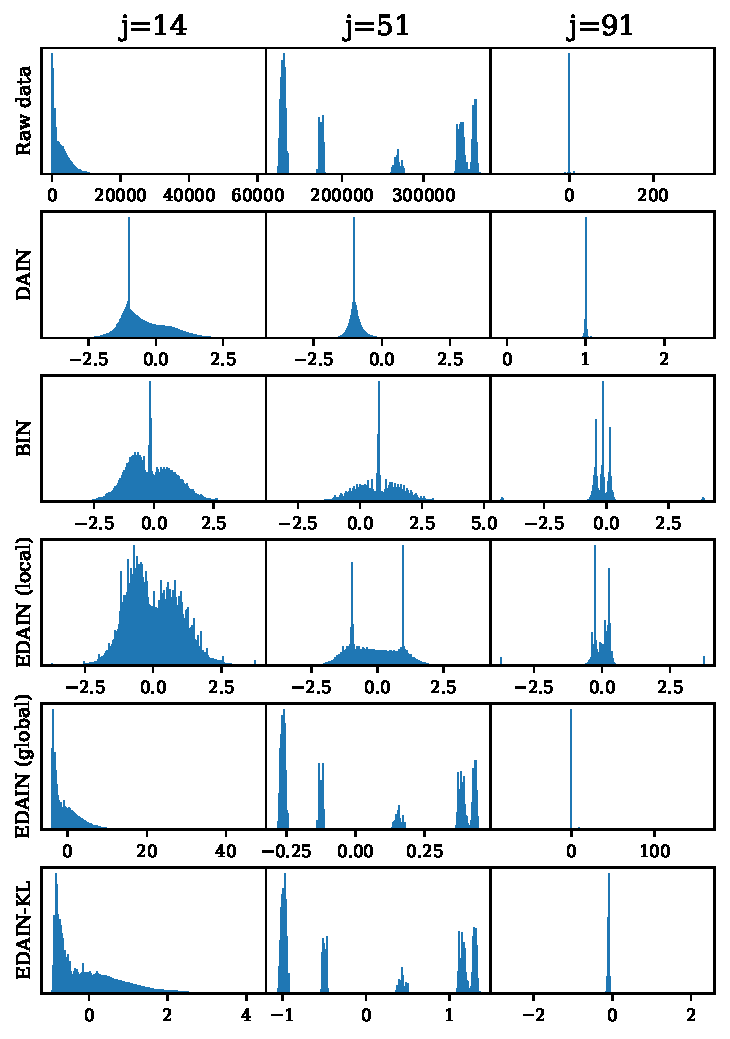
\includegraphics[scale=1]{figures/lob_example_transformations.pdf}
\end{center}
\caption{
    Examples of applying the different preprocessing methods to three different predictor
    variables from the FI-2010 \ac{LOB} dataset. In each plot, we consider the
    data points
    $\mathcal{X}=\left\{x^{(i)}_{t,j}\right\}_{i=1,2,\dots,N,t=1,2,\dots,T}$,
    where $j$ is specified in the column title.
    The 14$^{\textrm{th}}$, 51$^{\textrm{st}}$ and 91$^{\textrm{st}}$ predictor variables
    were chosen because they illustrate the different types of distributions found in
    the \ac{LOB} dataset.
    The preprocessing method used in each plot is specified by the left row title, where the top
    row shows the unprocessed, raw data. The $x$-axes show the variable values and the
    $y$-axes show the probability density.
}
\label{fig:lob_examples}
\end{figure}
% }}}

% EDAIN
\section{EDAIN}% {{{
\label{sec:EDAIN-discuss}

Based on the results observed in \cref{ch:Results},
we now present some insights related to the performance of the proposed
\ac{EDAIN} method, considering both its local-aware and global-aware modes.
As the local-aware \ac{EDAIN} resembles the
\ac{DAIN} and \ac{BIN} methods, and the global-aware \ac{EDAIN} method works similarly
to \ac{EDAIN-KL}, this discussion is expanded to compare all of these methods. In doing this,
we provide a holistic explanation for several of the observations related to
the methods' performance made in \cref{ch:Results}.
This explanation is augmented  with illustrative plots showing how the different preprocessing
methods transform real-world data.
Lastly, limitations of the \ac{EDAIN} layer are discussed.

\subsection{Local vs.\ global normalization}%
\label{sub:local_vs_global}

In \cref{sub:amex_res}, we made four observations about the performance of the adaptive
preprocessing methods on the two datasets:
\begin{enumerate}[(i)]
    \item The \ac{BIN}, \ac{DAIN}, and local-aware \ac{EDAIN} methods
        all performed relatively well on \ac{LOB} dataset.
    \item The EDAIN-KL method, standard scaling, and global-aware EDAIN method performed
        relatively poorly on the \ac{LOB} dataset.
    \item The global-aware \ac{EDAIN} method performs well on the synthetic dataset
        and the Amex dataset, outperforming all the other methods.
    \item The \ac{DAIN} and \ac{BIN} methods perform poorly on the synthetic dataset
        and the Amex dataset, even being outperformed by standard scaling.
\end{enumerate}
We now present some insight on the difference between local-aware and global-aware
normalization, which can explain why these phenomena occur.
%
First of all, we note that the \ac{BIN}, \ac{DAIN} and local-aware \ac{EDAIN} methods are
all local-aware as the normalization applied also depends on instance-specific summary statistics.
On the other hand, standard scaling, \ac{EDAIN-KL}, and the global-aware \ac{EDAIN} methods are
all global-aware because they all apply the same transformation to each sample. This categorisation
correlates with observations (i) and (ii): All the local-aware methods perform well on the
\ac{LOB} dataset, while the global-aware methods perform poorly.
This can be explained by the nature of the \ac{LOB} dataset: It contains limit orders from several
different company stocks, which gives rise to a mixture of data generation mechanisms within the
data. Aiming for a global normalization where all the samples are normalized equally does not bode
well for performance in such a case, hence observation (ii). Instead, it would make more sense to
condition the normalization on what data generation mechanism, or mode in the data, the sample
originated from, which is what the local-aware adaptive preprocessing methods
all learn to do during training. As such, it is expected that they perform better on this dataset,
compared to the preprocessing methods that treat all the samples the same, hence observation (i).
All this is clearly illustrated with the 51$^{\textrm{st}}$ predictor variable
in \cref{fig:lob_examples}:
The three local-aware methods are able to condition the normalization on which
of the five modes the sample came from, which allows them to transform all the samples into a common
unimodal representation space. The two global-aware methods, however, are not able to do this,
leading to a multimodal distribution after the transformation, which the neural network might
struggle to process.

We now turn our attention to the synthetic datasets and the Amex dataset, where
all the local-aware methods performed poorly according to observation
(iv), but the global-aware \ac{EDAIN} method performed very well, according
to observation (iii).
Unlike the \ac{LOB} dataset, the data generation mechanism for the Amex and synthetic data
is more global, especially in the synthetic data where we just have a single
data generation mechanism. Therefore, the relative ordering between the samples matters across
the whole distribution, not just around each mode as is the case for the \ac{LOB} dataset.
As such, it makes more sense to aim for a global instance-agnostic
normalization scheme, where all the samples are transformed by the same monotonic function,
such that their relative ordering is preserved.
This might explain observation (iv) as the \ac{DAIN} and \ac{BIN} methods do the opposite of this.
Therefore, even standard scaling outperform these methods as it shifts and
scales the data without changing the relative order of the samples.
It also explains observation (iii) as the global-aware \ac{EDAIN} method is a very flexible
transformation that can handle both the outliers and skewness present in the Amex dataset and
the synthetic dataset, all while preserving the relative order of the samples.
% Some notes:
% It’s to do with “local” vs “global” normalization. In amex data, batches aren’t
% really that different. They’re just “random samples” from a global
% distribution. Therefore, it makes more sense to aim for a global batch-agnostic
% normalization procedure, such as the EDAIN method I’ve implemented, and this is
% why DAIN and BIN does not work that well. On the other hand, for LOB dataset,
% have stocks from different companies and distributions are very multimodal,
% illustrating the difference in statistics between e.g. companies. On such
% problems, makes more sense to aim more more “local” mode-aware optimization,
% and reason why DAIN and BIN performs better

% Re-point-out that all the methods in Amex table improves upon DAIN and BIN
% Do some discussion in this, with silver lining that it's because latter are local-aware
% wheras Amex data follows global distribution, and very little multimodal nature, so from
% similar data generation mechanisms

\subsection{Examples}%
\label{sub:Examples}

In \cref{fig:lob_examples}, we highlight some example transformations from the adaptive
preprocessing methods.
The three local-aware methods, \ac{DAIN}, \ac{BIN} and local-aware \ac{EDAIN}, are all able
to transform the multimodal distribution in the second column into a more unimodal one,
but the \ac{BIN} method and local-aware \ac{EDAIN} method can also handle the skewness,
especially when compared to \ac{DAIN} when considering the $j=14$ variable.
We also notice that \ac{EDAIN} is better at centring the data to mean 0, compared to \ac{BIN}
and \ac{DAIN}. However, this may be due to the standard scaling applied before feeding the data
into the \ac{EDAIN} method to avoid numerical errors in the power transform sublayer.

We can also see the difference between  the local-aware and global-aware preprocessing methods in
\cref{fig:lob_examples}.
The local-aware methods are all able to turn the multimodal distribution into a more unimodal
one, while the global-aware methods mostly just change the scale and shift of the overall
distribution to make the range of values more standardized, but they do not change the shape of the
multimodal distribution much. However, they are better at transforming the unimodal distributions
in the first and third column. For example, both global-aware \ac{EDAIN} and \ac{EDAIN-KL}
are able to flatten the histogram to some degree and remove the outliers in the far-right of the
tail for $j=14$, with \ac{EDAIN-KL} being better at this due to its objective being based on how
Gaussian the transformed data is.

% Learns whether to apply a tanh activation or not, and as saw in \ac{PREPMIX-CAPS}, often mixture
% of tanh and standard scaler, so adaptive version???

\subsection{Limitations}%
\label{sub:Limitations}

One limitation of the \ac{EDAIN} layer is its many hyperparameters. We need to specify the
learning rate modifiers for the outlier removal, shift, scale and power transform sublayers
during training. Otherwise, training might be unstable.
Additionally, if we pass extreme values to an untrained \ac{EDAIN} layer, the gradients computed
for the power transform sublayer might produce \texttt{NaN}s due to numerical errors. To avoid
this, we apply standard scaling to the data before passing it to
the \ac{EDAIN} layer for training.
Another limitation arises when coupling the training of the \ac{EDAIN}
layer together with the training of the neural network model: If one wants to use a different
neural network architecture for a given task, the \ac{EDAIN} layer will need to be retrained as the
learned transformations might depend on the specific deep neural network architecture used.
This last limitation also applies to the \ac{BIN} and \ac{DAIN} layers, but is not present in
\ac{EDAIN-KL}.

% }}}

% EDAIN-KL
\section{EDAIN-KL}% {{{
\label{sec:EDAIN-KL-discuss}

% Note: Don't need subsection on performance; Can instead briefly mention that this method
%       performs poorly in the introduction with 2-3 sentences, then move onto discussing
%       the other aspects of this method

We now discuss the second proposed preprocessing method of this thesis, the \ac{EDAIN-KL} method.
We start this section by looking at some example transformations from this
preprocessing method. Then, we look at a big advantage of \ac{EDAIN-KL} when it comes to applying
it to unsupervised learning problems or for preprocessing data for non-neural-network models.
Finally, we look at some of the limitations of this preprocessing method, including a discussion
on its performance on the Amex dataset and \ac{LOB} dataset.

\subsection{Examples}%
\label{sub:Examples}

In the last row of \cref{fig:lob_examples}, we can see some example transformations from the
\ac{EDAIN-KL} method.
From the $j=14$ and $j=91$ plots, we see that the \ac{EDAIN-KL} method is able to handle outliers
well, as most of the low-density areas in the raw data has been pushed closer to the higher
density areas of the histogram. These observations are also present for variable 1
in \cref{fig:synth_examples}.
In \cref{fig:lob_examples} the skewness in variable $j=14$ is handled to some degree as well,
but the histogram still do not resemble that of a normal distribution. However, \ac{EDAIN-KL}
handles the skewness in variable 3 in \cref{fig:lob_examples} very well.
In the $j=51$ plot in \cref{fig:lob_examples}, we see that the \ac{EDAIN-KL} method
is not able to preprocess the multimodal data well, as it looks very similar to the raw data.
This is one of its weaknesses as it does not have a local-aware mode.

\subsection{Advantages}%
\label{sub:edain_kl_advantages}

% Unsupervised learning, no need to have responses
\ac{EDAIN-KL} is fully unsupervised, that is,
we no not need the target labels  to fit the bijector. This
allows the method to preprocess data for unsupervised machine learning tasks
such as dimensionality reduction, clustering, or anomaly detection.
Additionally, these tasks do not need to fit into the deep learning
framework because the \ac{EDAIN-KL} bijector is trained separately from
the neural network. This allows \ac{EDAIN-KL} to be used
in a wider range of problems compared to \ac{EDAIN}, which also includes supervised
non-neural-network machine learning models.
However, as the scope of this thesis did not cover non-neural network models
nor unsupervised learning problems, the effectiveness of the \ac{EDAIN-KL}
preprocessing method has not been evaluated on such tasks. 
Regardless, the rest of this subsection looks at how \ac{EDAIN-KL} might be useful,
and provide benefits beyond traditional methods like standard scaling,
in such scenarios.

% Linear regression OLS example
One especially relevant application of \ac{EDAIN-KL} is performing linear regression with
\ac{OLS}.
% In linear regression, we typically assume the error terms
% $\epsilon_1,\dots,\epsilon_N$ follow a normal distribution \citep{wasserman}. Thus, if we want
% to apply \ac{OLS} to a dataset where the covariates follow a very skewed distribution or one with
% a lot of outliers, we can reduce the effect of incorrectly assuming Gaussian errors by first
% preprocessing our data with the \ac{EDAIN-KL} method to reduce the effect of outliers and reduce
% the skewness with the power transform sublayer. 
%
In linear regression, we typically assume the response variable $Y$ can be expressed as a linear
combination of the predictor variables $X_1,X_2,\dots,X_d$ \citep{wasserman}. However, this
assumption is not always reasonable as we might have a relationship of the form
$Y=\log(X_1)+\dots+\log(X_d)+\epsilon$ or a mixture of more complicated transformations:
$Y=f_1(X_1)+\dots+f_d(X_d)+\epsilon$.
There might also be outliers present. In such a case,
simple power transformations such as what \cite{boxcox} and \cite{yeoJohnson} propose
might not be sufficient. Instead, one could preprocess the covariates with \ac{EDAIN-KL} first
to correct for this non-linearity as much as possible using its four flexible sublayers to
approximate $f_1^{-1}, f_2^{-1},\dots,f_d^{-1}$.

Another relevant example is
performing dimensionality reduction with \ac{PCA}. This method is usually sensitive to the
scale of the different variables, so one typically applies standard scaling to ensure all the
variables are treated fairly in the \ac{PCA} routine. However, this does not remove potential
skewness
and outliers that may be present in the dataset. For this, one could normalize the data with
\ac{EDAIN-KL} first as this layer can both standardize the data like standard scaling, but
also remove skewness and reduce the effects of outliers.

% TODO: squeeze in the second avantage: Can swap out the neural network or try
% different architectures, without needing to retrain the \ac{EDAIN-KL} layer
% as seperate... Can't do this with the EDAIN layer
% Don't add the adaptive layer overhead during training of the final neural network with this...

\subsection{Limitations}%
\label{sub:Limitations}

% Architecture-based limitations
% * Cannot do local-aware mode
% * Outlier removal transformation simplified from \ac{EDAIN} method to make the
%   inverse transformation into an analytic expression
The \ac{EDAIN-KL} layer cannot run in local-aware mode like the \ac{EDAIN} layer.
As we saw in \cref{sub:opt_with_kl}, to train the \ac{EDAIN-KL} layer, we need analytic and
differentiable expressions for the inverse of each of the sublayers: outlier removal, shift,
scale, and power transform. Recalling how the local-aware \ac{EDAIN} architecture presented
in \cref{sub:edain_arch} used summary representations
\begin{equation}
    \mu_\bfx^{(i)}=\frac{1}{T} \sum^{T}_{t=1} \bfx^{(i)}_t  \quad\textrm{ and }\quad
    \sigma_\bfx^{(i)}=\sqrt{\frac{1}{T}  \sum^{T}_{t=1} \left(\bfx^{(i)}_t- \mu_\bfx^{(i)} \right)^2}
\end{equation}
in the expressions for the shift and scale operations, respectively, we would need to be able to
invert these summaries to get an expression for the inverse shift and scale operations. However,
that is not possible as taking the sum of the data along the time-axis discards information.
Therefore, with a local-aware shift and scale operation, we cannot fulfil the requirements
we set out in \cref{sub:opt_with_kl} for optimising the layer with \ac{KL-divergence}.
This constrains the \ac{EDAIN-KL} layer to only being able to perform global-aware normalization,
so it cannot be made suitable for highly multimodal datasets such as the \ac{LOB} dataset.

% Performance, need to motivate why EDAIN-KL is not doing well on the LOB dataset
% Discuss why perform poorly here: Can theoretically generalise standard scaling,
% but requires learning the shift and scale parameters for all the variables, and
% it is not guided by the loss gradients like EDAIN method, so might waste time
% trying to standardize variables that are not even important to predicting the
% response, while leaving the important variables untouched, as optimised with
% how close dataset is to standardized normal, where all variables weighted
% equally, but clear variable importance difference when it's actually time to
% train the neural network. This disparity ...
%
% Point out that even worse than standard scaling even though it should be able to generalize
% standard scaling in theory, so even more flexible. Why worse?

Another limitation of the \ac{EDAIN-KL} method is its relatively poor performance on the two
real-world datasets that we evaluated the method on. Despite its good
performance on the synthetic dataset and it outperforming
min-max scaling and standard scaling on the
\ac{LOB} dataset, its performance is nowhere near that of the local-aware preprocessing
methods on the \ac{LOB} dataset. Additionally, it underperforms standard scaling on the Amex dataset despite
the \ac{EDAIN-KL} layer being designed to be a generalisation of standard scaling through
its flexible shift and scale sublayers. One possible reason for this might be the high
dimensionality of the dataset, with $d=188$ predictors. As the \ac{EDAIN-KL} bijector is trained
based on the \ac{KL-divergence} between the dataset and a transformed normal distribution, instead
of using the loss function related to the prediction task, the variable prioritisation will be
completely different when compared to \ac{EDAIN}. This may cause
the \ac{EDAIN-KL} layer to waste time determining how to transform variables that are not
important for the prediction task, while possibly neglecting the most important variables,
as it has no information about the variable importance due to the training process being separated
from the neural network training.

% Others
% * Many hyperparameters to tune,
% * Power transform numerical errors while computing gradients, sometimes need
%   to be combined with Z-Score scaling to avoid this
% * separate training procedure, adds overhead to training, but also several
%   advantages as discussed above
% TODO: include this???
% Some other limitations are the many hyperparameters required to tune, as the learning rates for
% all four sublayers need to be fine-tuned. Additionally, the power-transform layer usually
% encounters numerical errors when its gradients are computed, causing training to need to be
% restarted or the power transform layer turned of or configured with a very low learning rate.

% }}}

% PREPMIX-CAPS
\section{PREPMIX-CAPS}% {{{
\label{sec:PREPMIX-CAPS}

% TODO: comment on why might not be that much better than just standard scaling:
% * E.g. potential that all the important features are in one clustering, and other features
%   not that important, so does not matter what preprocessing method apply to them
% * But in the validation split method, see that outperforms standard scaling across time
%   on some of the splits, so somewhat good
% * Additionally, interesting to see the mixture of the preprocessing methods selected for
%   the method. See appendix ....
% * Comment from Leonie as well on this:
%   """
%     I skipped some parts so I don’t know if this is included anywhere else, but
%     maybe mention here the hypothesis that we had, why the results of PREPMIX-CAPS
%     and standard scaling are so similar, i.e. almost identical 
%   """

We now look at the third proposed preprocessing method, the \ac{PREPMIX-CAPS} procedure.
Performance-wise, \ac{PREPMIX-CAPS} achieves the second-best performance on the Amex dataset
out of all the methods tested, outperforming standard scaling slightly while underperforming the
proposed global-aware \ac{EDAIN} method. However, the method comes with several limitations, which
we will now discuss.

\subsection{Limitations}%
\label{sub:Limitations}

One of \ac{PREPMIX-CAPS}'s biggest limitations is its computational
inefficiency. As discussed in \cref{sub:prep_determine}, to determine what
preprocessing method to use for each cluster of predictor variables, $(m-1)k+1$
experiments need to be ran. Even though this search can be parallelised across
multiple \acp{GPU}, it still takes a significant amount of time, especially
compared to the other preprocessing methods such as Standard scaling and the
low overhead of \ac{EDAIN}, \ac{BIN} or \ac{DAIN}. This problem becomes even worse
when it comes to tuning the hyperparameter $k$, that is, the number of
clusters. For each candidate value for $k$, we need to run all the $(m-1)k+1$
experiments again.  In addition to the slow fit procedure, the preprocessing
method also leads to slow convergence when fitting the neural network.  As we
saw \cref{fig:amex_performance}, with the \ac{PREPMIX-CAPS} procedure, the
neural network took a bit more than twice as many epochs to converge compared
to with standard scaling or \ac{EDAIN}.  A third limitation is that the method
cannot perform local-aware transformations like the \ac{EDAIN}, \ac{BIN} and
\ac{DAIN} layers, as the procedure is not an adaptive one. It might therefore
not be suitable for highly multimodal datasets unless one of the $m$ static
preprocessing techniques can handle multiple modes well.

% TODO: talk about how very similar performance to standard scaling in \cref{fig:amex_performance_metric}, so might just use standard
%       scaling on the important variables...

% }}}

\section{Conclusion}%
\label{sec:Conclusion} %%% Conclusion {{{

In this chapter, we discussed the effectiveness of the main contributions of
this thesis--the \ac{EDAIN}, \ac{EDAIN-KL}, and \ac{PREPMIX-CAPS}
preprocessing techniques--by explaining the results observed in
\cref{ch:Results} and looking at the methods' limitations.
We started by
considering \ac{EDAIN} and similar methods, where we discussed why the local-aware
adaptive preprocessing methods all performed well on the \ac{LOB} dataset. This
was likely because they were able to transform the multimodal predictor
variables into a common unimodal representation space. We also saw this happening
in practice with the example transformation plots.
We also discussed potential reasons for why the local-aware methods did not perform well on Amex
dataset or on the synthetic data. In these datasets the relative ordering between the samples
matter more across the whole distribution, so global-aware
preprocessing methods perform better.  The skewness and outliers present in the
datasets may also explain why the global-aware \ac{EDAIN} performed so well on
these two datasets.

% Limitations of each method, and some advantages
We also saw how both the \ac{EDAIN} and \ac{EDAIN-KL} methods
were limited by their many hyperparameters that had to be tuned, as well as
possible numerical errors that may occur in the gradients of the power transform sublayer when
transforming extreme values.  Moving onto the \ac{EDAIN-KL} method, we discussed
its advantage when working with unsupervised learning tasks or with non-neural
network models, such as \ac{OLS} regression models or \ac{PCA} models for
dimensionality reduction. However, the \ac{EDAIN-KL} is limited by not having a
local-aware mode, and it performs somewhat poor on the two of the three datasets
considered, possibly due to its training objective being disjoint from the task
objective.
Finally, we briefly discussed the \ac{PREPMIX-CAPS} routine, mainly
focusing on its major limitation which is its computational inefficiency.


% }}}

% TODO:
% * Nice discussion point is how standard scaling across time outperforms the other standard scaling
%   method, and how this can be because the change in distribution from one
%   timestep to next conveys important information for each customer, so if
%   standard scaling across both time and dimension, then discard this
%   information
% * If I want to add this discussion point, I should also include the other
%   standard scaling method in my benchmarking experiments in the results chapter

% TODO:
% * Nice discussion point about synthetic: On the local-aware EDAIN, it did not merge the
%   modes in the synthetic data because the relative ordering of the data points (monotonicty)
%   was what affected the response. However, in the LOB dataset, it was the relative mode-based
%   variations of each data point was carried the important imformation for classification, hence
%   modes being merged in this case

%%%%%%%%%%%%%%%%%%%%%%%%%%%%%%%%%%%%%%%%%%%%%%%%%%
\chapter{Conclusion} %%%%     Conclusion      %%%%
%%%%%%%%%%%%%%%%%%%%%%%%%%%%%%%%%%%%%%%%%%%%%%%%%%
\label{ch:Conclusion}

To conclude the thesis, we provide summaries of the three novel preprocessing methods proposed,
the results we observed when applying them to three different datasets, and related
discussions. Afterwards, we clearly list the main contributions of the thesis, which includes
three novel preprocessing methods and a new synthetic data generation algorithm. Then we
discuss some possible future work that builds upon our contributions.

\vspace*{-10pt} % reduce number of pages hack :/

% Summary (1 - 1+1/2 pages of summary of thesis)
\section{Summary}% {{{
\label{sec:Summary}

% Summarise the three methods proposed
% EDAIN:
% * Inspired by DAIN and BIN \cite{dain} and \cite{bin}
% * prepend this adaptive preprocessing layer to the deep sequence model that will be used for the task,
%   and unknown parameters of both optimised simultaneously in end-to-end fashion while backprop
% * consists of four adaptive sublayers: outlier removal, shift, scale, and  power transform
% * two different modes: in the global-aware mode, the same shift and scale is
%   applied to all samples, while in local-aware mode, the amount of shifting and
%   scaling might also depend on summary statistics computed for the sample. The mode also affects
%   how the mean estimate is computed in the adaptive outlier sublayer.
% * The unknown parameters of the four sublayers are optimised with backpropagation while the
%   deep sequence model is being trained
In this thesis, we propose three novel preprocessing methods for multivariate time-series data.
The first method, \textit{\acl{EDAIN}} (\acs{EDAIN}), is based on existing work by \cite{dain} and
\cite{bin}. It has four adaptive sublayers: an outlier removal layer, a shift layer,
a scale layer, and a power transform layer. It also has two normalization modes: In the local-aware
mode, the amount of shifting and scaling applied to each sample also depends on summary
statistics computed for that sample; in the global-aware mode, the same amount
of shifting and scaling is applied to each sample. 
% All the unknown parameters of the preprocessing
% layer is optimised in an end-to-end fashion through backpropagation by attaching the \ac{EDAIN}
% layer in front of the deep sequence model that is to be trained.
% EDAIN-KL:
% * similar architecture as EDAIN and also inverted, but instead of attach to deep sequece model,
%   optimised seperately using ideas from normalizing flows
% * The layer is trated as an invertible transformation and we optimise its parameters
%   by minimize the \ac{KL-divergence} between the empirical distribution and a multivariate
%   independent normal distribution, our base distribution, that has been transfromed by the
%   \ac{EDAIN-KL} layer. Then, when it is time to normalize the data, we apply the inverse \ac{EDAIN-KL}
%   transformation to each sample in the dataset.
The second method we propose is \textit{\acl{EDAIN-KL}} (\acs{EDAIN-KL}).
Its architecture has the same four sublayers of
\ac{EDAIN}, but they are simplified slightly and are all inverted. Unlike \ac{EDAIN}, the
unknown parameters of \ac{EDAIN-KL} are optimised separately from the deep neural network by
using ideas from normalizing flows. % The preprocessing layer is treated as an invertible
% transformation we optimise its parameters by minimizing the \ac{KL-divergence} between the
% empirical distribution of the dataset and a multivariate normal
% distribution--our base distribution--that has been transformed by the
% \ac{EDAIN-KL} layer.
Then, to normalize the data, we apply \ac{EDAIN-KL}' inverse transformation to each sample.
% PREPMIX-CAPS:
% * auaomated pipeline for selecting which static preprocessing method to apply to each variable
% * done by first clustering the predictor variables, and then running several experiments in parallel
%   to select the optimal preprocesing method for each cluster of variables. This method then applied to each
%   variable in that cluster
The third preprocessing method we propose is named \textit{\acl{PREPMIX-CAPS}} (\acs{PREPMIX-CAPS}).
This method is an automated pipeline for selecting which static preprocessing method to apply
to each variable, which is done using clustering and running several experiments in parallel to
determine which preprocessing method to apply in each cluster.

% Summarise the experiments conducted (3 datasets)
% The methods were then evaluated on three different datasets.
% * First synthetic data considered, where we saw how the global-aware \ac{EDAIN}
%   method almost performed as well as if the data was perfectly normalized to a
%   standard Gaussian
% * (Mention how generated very irregular data)
% * We then assessed the methods on the Amex dataset, where we found the
%   global-aware methods work best, with global-ware \ac{EDAIN} outperforming all
%   the other methods
% * Then looked at the FI-2010 \ac{LOB} dataset, where the local-ware methods performed the best,
% with all of \ac{DAIN}, \ac{BIN} and proposed local-ware \ac{EDAIN} performing very closely at top,
% but latter with a slightly higher mean performance
The three proposed methods were evaluated on three different
datasets with very different characteristics. They were also compared to existing work by
\cite{dain} and \cite{bin}, and to other conventional preprocessing methods.
We first considered a synthetic dataset,
 configured to have very irregularly-distributed data. 
When evaluating the performance of the different preprocessing methods on this dataset, we find
the global-aware \ac{EDAIN} method to perform very closely to the gold-standard method.
We also evaluated all the methods on the Amex dataset, where we also find the
global-aware \ac{EDAIN} method to clearly outperform all the other methods. On
this dataset, the local-aware methods perform poorly. Finally, we looked at
the methods' performance on the FI-2010 \ac{LOB} dataset, where the local-aware
methods all perform very well, compared to the global-aware ones.
The proposed local-aware \ac{EDAIN} method has slightly higher mean metric values
than the \ac{DAIN} and \ac{BIN} methods, but there was no clear-cut best performing method.
% Summarise the discussion, including advantages, main results, **limitations** etc.
% Discussion:
% * discussed potential reasons for why the local-aware performed so well on the LOB data, but poorly on Amex data, and why
%   global-aware methods worked best on Amex data
% * also augmented this discussion with visual plots of the key differences and
%   cahracteristics of the two approaches to normalizing time-series data
After evaluating all the methods, we discussed potential reasons for why the local-aware methods
all perform very well on the \ac{LOB} dataset, but poorly on the Amex dataset,
which is likely due to the different underlying data generation mechanisms in each dataset.
This discussion was augmented with illustrative plots that showed how the different
preprocessing methods transformed the data distribution in practice.
Afterwards, we looked at some of the limitations of each of the three preprocessing
methods we propose.

% Also talk about main limitations of this study in general
% * Only applied to two real-world datasets, and experiments with synthetic
%   dataset were far from exhaustive
% * Only considered one type of sequence model architecture, a RNN model with GRU cells
% * ...

% }}}

% Main contributions (just bullet point of everything, underlining them very clearly)
\section{Main contributions}% {{{
\label{sec:Main contributions}

The main contributions of this thesis can be summarised as follows:
\begin{itemize}
    \item Proposed a new adaptive preprocessing method, named \ac{EDAIN}.
        This method extends the \ac{DAIN} layer proposed by \cite{dain} with an
        adaptive outlier removal sublayer and a power transform sublayer. It showed comparable
        performance to existing methods on the FI-2010 \ac{LOB} dataset.
    \item Further extended the proposed \ac{EDAIN} method with a novel global-aware
        mode, which allows it to efficiently normalize data from more unimodal data generation
        mechanisms, such as what underlies the Amex dataset. The global-aware \ac{EDAIN} method
        outperforms all the other methods, including those \cite{dain} and
        \cite{bin} propose, on both the Amex dataset and the synthetic dataset. On the latter dataset,
        it almost performs as well as the gold-standard.
    \item Proposed a second adaptive preprocessing method, named \ac{EDAIN-KL}.
        Like \ac{EDAIN}, this method can normalize skewed data with outliers, but
        in an unsupervised fashion and can be used in conjunction with non-neural-network models.
    \item Proposed a third automated preprocessing method, named \ac{PREPMIX-CAPS}.
        This method is an automated procedure for selecting how best to apply a
        mixture of preprocessing methods to a dataset.
    \item Proposed and implemented a novel and efficient synthetic multivariate
        sequence data generation algorithm. This generation mechanism has many
        desirable properties for generating synthetic data for research
        into preprocessing methods, such as allowing the user to specify arbitrary
        \acp{pdf} to generate samples from.
    \item Applied two state of the art preprocessing methods proposed by \cite{dain} and \cite{bin}
        on two new datasets, the Amex dataset and the synthetic data, in
        addition to the already considered FI-2010 \ac{LOB} dataset. Their performance
        on the three datasets was analysed and compared to that of the
        preprocessing methods proposed in this thesis. This led to interesting insight on
        local-aware vs.\ global-aware approaches to data normalization.
\end{itemize}

% }}}

% Future work
\section{Future work}% {{{
\label{sec:Future work}

% Evaluate on other sequence models
In this thesis, we only considered \ac{GRU} \ac{RNN} models, but there are other types of
deep sequence models such as \acp{LSTM} \citep{lstm} and the more 
sophisticated transformer architecture proposed by \cite{attention}. It is unknown how effective
the proposed adaptive preprocessing techniques are when using these alternative architectures, so
this would be a suitable and relevant extension to the project. Additionally, 
\cite{dain,rdain} found their adaptive local-aware preprocessing methods to significantly improve
the predictive performance of conventional feed-forward neural networks, so it would be
interesting to assess the effectiveness of the two modes of \ac{EDAIN} when using this
architecture.
% EDAIN (global) on non-sequence tasks
In fact, the global-aware \ac{EDAIN} method do not make any assumption on the
dataset being a multivariate time-series as we do not compute summary representations of each
sample. Therefore, it could also be used to preprocess non-sequence data such as conventional
tabular data for use in  feed-forward neural networks.

% Handling missing values with BRITS model
When applying our methods to the Amex dataset, we treat the missing values in
a very straightforward manner by simply replacing them with predetermined constants.
\cite{brits} propose a data-driven adaptive imputation method for sequence data
that makes minimal assumptions on the data generation mechanism.  Their method
integrates the imputation procedure into the \ac{RNN} model and learns how to
fill the missing values while training the neural network with backpropagation,
just as how \ac{EDAIN} learns how to preprocess data while the model is being
trained. As \cite{nawi,brits} observe, missing values are very common in
real-world sequence datasets, which we also confirmed during our \ac{EDA} of
the Amex dataset. Therefore, extending the proposed \ac{EDAIN} method with the
missing value imputation technique proposed by \cite{brits} could increase
the effectiveness  of our work in real-world applications.

% EDAIN-KL on unsupervised tasks
In  \cref{sub:edain_kl_advantages}, we talked about \ac{EDAIN-KL}'s potential
advantages when applied in unsupervised learning problems or for preprocessing data
for non-neural-network models. However, the effectiveness of the \ac{EDAIN-KL}
method in these settings was never tested and evaluated.
This deserves further investigation.

% More investigation of PREPMIX-CAPS
The \ac{PREPMIX-CAPS} method has a lot of potential for deriving new insight
related to automated preprocessing of predictor variables, which was not
investigated in depth in this thesis. For instance, after clustering the
predictor variables and determining the optimal static distribution
transformation to apply to each variable, one could reason about the characteristics
of the variables with the preprocessing technique selected for
them in mind. This way, one can build insight on what specific characteristics of a
variable makes a certain preprocessing method work well.
% Working toward replacing brute-force search with heuristic-based selection
This builds towards eliminating the main limitation of \ac{PREPMIX-CAPS}, which
is the brute-force search for the optimal preprocessing technique. In building
this insight, one could start working towards developing heuristics for
automatically selecting the preprocessing methods, without needing to train a
neural network.

% }}}

%%%%%%%%%%%%%%%%%%%%%%%%%%%%%%%%%%%%%%%%%%%%%%%%%%%%%%%%%%%%%%%%%%%%%%%%%%%%%%%%
%%%%%%%%%%%%%%%%%%%%%%%%%%%%%%%% Appendix %%%%%%%%%%%%%%%%%%%%%%%%%%%%%%%%%%%%%%
%%%%%%%%%%%%%%%%%%%%%%%%%%%%%%%%%%%%%%%%%%%%%%%%%%%%%%%%%%%%%%%%%%%%%%%%%%%%%%%%
% Appendix misc {{{
\clearpage
 %% reset page counter and start appendix pages with A
\pagenumbering{arabic}
\renewcommand*{\thepage}{A\arabic{page}}

%% Appendix goes here
\appendix
% }}}

\chapter{Implementation and hardware notes}%
% {{{
\label{cha:imp_notes}

In this chapter of the appendix, we present the deep learning framework that was used to
implement, train and evaluate all the deep neural networks used in this thesis. We also
give an overview of how the thesis code is structured. Finally, we provide the hardware
specifications of the machine that was used to run all the experiments.

\section{Deep learning frameworks used}%
\label{sec:Deep learning frameworks used}

For the whole of this thesis, we used the PyTorch deep learning framework,
developed by \cite{pytorch}. Additionally, the probabilistic programming framework Pyro,
developed by \cite{pyro}, was used for implementing parts of the \ac{EDAIN-KL} model.

\section{Repository overview}%
\label{sec:Repository overview}

All the code written as part of this thesis is publicly available at
\url{https://github.com/marcusGH/automated-preprocessing-for-deep-neural-networks}. Excluding
code from Jupyter notebooks, the repository contains 5027 lines of Python code that were all
written as part of this thesis, except where otherwise stated.

\begin{itemize}
    \item \texttt{notebooks/}
           contains several Jupyter notebooks that was used to prototype plots
                and code before it was rewritten into Python scripts and put in the \texttt{src/}
                directory.
    \item \texttt{reports/} 
            contains the latex code for this thesis and the poster.
    \item \texttt{scripts/}
            contains all the Python scripts that were use to create the plots
                presented in this thesis, as well as Bash shell scripts used to run the
                hyperparameter tuning experiments.
    \item \texttt{src/}
        \begin{itemize}
            \item \texttt{experiments/}
                contains the main \texttt{run\_experiment.py} script as well as related
                experiment configuration files that contains many of the hyperparameters used
                for the experiments. This directory also contains other miscellaneous scripts used
                to run the synthetic data experiments, among others.
            \item \texttt{lib/}
                contains utility functions used across the whole project, split across 8 different
                Python files. 
            \item \texttt{models/}
                contains the PyTorch code for all the \ac{GRU} \ac{RNN} models used in the
                experiments.
            \item \texttt{preprocessing/}
                contains four Python files: \texttt{adaptive\_transformations.py} contains the
                code for the \ac{DAIN} and \ac{BIN} method proposed by \cite{dain} and
                \cite{bin}, respectively. \texttt{mixture.py} contains code related to the
                \ac{PREPMIX-CAPS} procedure. \texttt{normalizing\_flows.py} contains code
                for the \ac{EDAIN} method, including all of its variants: local-aware, global-aware,
                and \ac{EDAIN-KL}. \texttt{static\_transformations.py} contains
                code for traditional preprocessing methods such as standard
                scaling and min-max scaling.
            \item \texttt{tests/} contains python scripts for unit testing parts of the code in
                \texttt{lib/}.
        \end{itemize}
\end{itemize}

\section{Hardware notes}%
\label{sec:Hardware notes}

All experiments were run on the \texttt{nvidia6} cluster offered by the Department of Mathematics
at Imperial College London. This machine is a \texttt{Asus ESC8000 G4} server with the following
specifications:
\begin{itemize}
    \item two 16-core CPUs of model \texttt{Intel(R) Xeon(R) Gold 6242 CPU @ 2.80GHz}
    \item 896 GiB of system memory
    \item eight GPUs of model \texttt{NVIDIA GeForce RTX 3090}, each with
        $24\;576~\textrm{MiB}$ of video memory (VRAM)
\end{itemize}

% }}}

\chapter{Hyperparameter tuning}%
% {{{
\label{cha:Hyperparameter tuning}

\section{Model architecture for the Amex dataset}%
\label{sec:hyp_amex_mod}

The \ac{GRU} \ac{RNN} architecture is based on a ``starter model'' found on the Kaggle competition
discussion page\footnote{
    \url{https://www.kaggle.com/competitions/amex-default-prediction/discussion}
} for the American Express default prediction competition, where the dataset
originate from \citep{amex-data}. The ``starter model'' architecture was initially
proposed by \cite{amex-starter}.

\section{Optimizer for the Amex dataset}%
\label{sec:hyp_amex_opt}

For the training the \ac{RNN} model on Amex dataset, we used a batch size of 1024.
This was chosen to give a good trade-off between the time required to train the model and
predictive performance. This model was also optimised with the Adam optimizer proposed by
\cite{adam}. This optimizer was chosen for its reputation of being an effective optimizer in
most cases. The learning rate was also set to $\eta=10^{-3}$ after testing what learning rate
from the set $H=\{10^{-1}, 10^{-2}, 10^{-3}, 10^{-4}\}$ gave the most stable convergence.
To momentum parameters $\beta_1$ and $\beta_2$ were set to their default values according to
the PyTorch implementation of the optimizer \citep{pytorch}.
For learning rate scheduler, the step size was set to $\gamma=\frac{1}{10}$ because this is
a natural step-size. For the milestones, we first tune the first step based on observing the
learning rate curve during training and setting the step epoch to ensure the performance did not
jump around too much. This was done until we got milestones at 4 and 7.
For the patience for the early stopper, the number $p_{\textrm{patience}}=5$ was chosen as a nice
non-zero number that was not too big.

\section{Hyperparameters of preprocessing methods for the Amex dataset}%
\label{sec:hyp_amex_prep}

\subsection{Adaptive preprocessing methods}

The \ac{BIN} method proposed by \cite{bin} and the \ac{DAIN} method proposed by \cite{dain} have
both never been applied to the Amex dataset before, so their hyperparameters should be tuned
for this dataset. We also tune the two modes of \ac{EDAIN} on this dataset. For all these
experiments, we run a grid-search with different combinations of the hyperparameters, specifically
the learning rate modifiers, using the validation loss from training a single model for 10
epochs on a 80\%-20\% split of the training dataset. We then pick the combination giving
the lowest validation loss. The grids use for the different preprocessing methods are:

\paragraph{BIN}%

We used the grids:

$H_{\beta}=\{10,1,10^{-1},10^{-2},10^{-6}\}$,

$H_{\gamma}=\{10,1,10^{-1},10^{-2},10^{-6}\}$, and

$H_{\lambda}=\{10,1,10^{-1},10^{-2},10^{-6}\}$.

The combination giving the lowest average cross-validation loss was found to be
$\eta_\beta=10$, $\eta_\gamma=1$, and $\eta_\lambda=10^{-6}$, giving 0.2234.

\paragraph{DAIN}%

We used the grids:

$H_{\textrm{shift}}=\{10,1,10^{-1},10^{-2},10^{-3},10^{-4}\}$ and

$H_{\textrm{scale}}=\{10,1,10^{-1},10^{-2},10^{-3},10^{-4}\}$.

The combination giving the lowest average cross-validation loss was found to be
$\eta_{\textrm{shift}}=1$ and $\eta_{\textrm{scale}}=1$, giving $0.2216$.

\paragraph{Global-aware EDAIN}%

We used the grids:

$H_{\textrm{scale}}=H_{\textrm{shift}}=H_{\textrm{outlier}}=H_{\textrm{pow}}=\{100,
10, 1, 10^{-1}, 10^{-2}, 10^{-3}\}$.

The combination giving the lowest average cross-validation loss was found to be
$\eta_{\textrm{shift}}=10^{-2}$,
$\eta_{\textrm{scale}}=10^{-2}$,
$\eta_{\textrm{outlier}}=10^{2}$, and
$\eta_{\textrm{pow}}=10$, giving $0.2190$.

\paragraph{EDAIN-KL}%

Note that due to numerical gradient errors in the power transform layers occurring for some
choices of power transform learning rates, the values considered are all low to avoid these
errors. We used the grids

$H_{\textrm{outlier}}=\{100, 10, 1, 10^{-1}, 10^{-2}, 10^{-3}\}$,

$H_{\textrm{scale}}=\{100, 10, 1, 10^{-1}, 10^{-2}, 10^{-3}\}$,

$H_{\textrm{shift}}=\{100, 10, 1, 10^{-1}, 10^{-2}, 10^{-3}\}$, and

$H_{\textrm{pow}}=\{10^{-7}\}$

The combination giving the lowest average cross-validation loss was found to be
$\eta_{\textrm{shift}}=10$,
$\eta_{\textrm{scale}}=10$,
$\eta_{\textrm{outlier}}=10^{2}$, and
$\eta_{\textrm{pow}}=10^{-7}$, giving $0.2208$.

\subsection{PREPMIX-CAPS}

% PREPMIX-CAPS
For the \ac{PREPMIX-CAPS} routine, we trained the \ac{GRU} \ac{RNN} model
using the hyperparameters specified in \cref{sec:hyp_amex_mod} using the \ac{PREPMIX-CAPS}
method with 7 different values for the number of clusters, $k \in \{2, 4, 6, 8, 10, 20, 30\}$.
The results are shown in \cref{fig:prepmix_tune}. As $k=20$ gave the best results, this is
the number of clusters used in the final benchmarking in \cref{ch:Results}.

\begin{figure}[htp]
    \begin{center}
        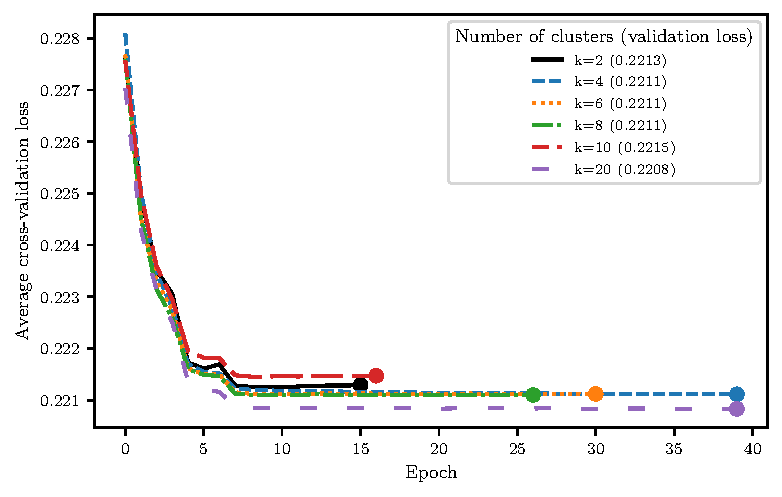
\includegraphics[scale=1]{figures/mixture-clustering-tuning.pdf}
    \end{center}
    \caption{Convergence rate and final average cross-validation loss for different $k$ parameters
    of the \ac{PREPMIX-CAPS} preprocessing method.}
    \label{fig:prepmix_tune}
\end{figure}

\section{Optimizer for the LOB dataset}%
\label{sec:hyp_lob_opt}

For the \ac{LOB} datasets, we used a \ac{GRU} \ac{RNN} architecture with the exact
same architecture as what \ac{DAIN} used when evaluating \ac{DAIN} on the same \ac{LOB} dataset.
This was to ensure a fair comparison to their work. For similar reasons, why also used the same
optimizer and learning rates as they did, giving us the RMSProp optimizer proposed by \cite{rmsprop}
with base learning rate $\eta=10^{-4}$. Since \cite{dain} did not use any early stoppers nor
learning rate schedulers, we also chose not to do this in our \ac{LOB} experiments.

\section{Hyperparameters of preprocessing methods for the LOB dataset}%
\label{sec:hyp_lob_prep}

The \ac{BIN} method proposed by \cite{bin} and the \ac{DAIN} method proposed by \cite{dain} have
already been applied to the \ac{LOB} dataset before, but only \ac{DAIN} have been applied
with the specific \ac{GRU} \ac{RNN} architecture we are using. Therefore, the learning rate
modifiers found by \cite{dain} will be used as-is, and the learning rate modifiers for
the remaining methods will be tuned. The details of this is presented here.
For all the learning rate tuning experiments, we used the first day of data from the FI-2010
\ac{LOB} for training and the data from the second day for validation. We then pick the
combination giving the highest validation Cohen's $\kappa$-metric.

\paragraph{BIN}

We used the grids:

$H_{\beta}=\{10,1,10^{-1},10^{-2},10^{-6},10^{-8}\}$,

$H_{\gamma}=\{10,1,10^{-1},10^{-2},10^{-6}, 10^{-8}\}$, and

$H_{\lambda}=\{10,1,10^{-1},10^{-2},10^{-6},10^{-8}\}$.

The combination giving the lowest average cross-validation loss was found to be
$\eta_\beta=1$, $\eta_\gamma=10^{-8}$, and $\eta_\lambda=10^{-1}$, giving $\kappa=0.3287$.

\paragraph{Global-aware EDAIN}%

We used the grids:

$H_{\textrm{scale}}=H_{\textrm{shift}}=H_{\textrm{outlier}}=H_{\textrm{pow}}=\{
10, 10^{-1}, 10^{-3}, 10^{-6}\}$.

The combination giving the lowest average cross-validation loss was found to be
$\eta_{\textrm{shift}}=10$,
$\eta_{\textrm{scale}}=10$,
$\eta_{\textrm{outlier}}=10^{-6}$, and
$\eta_{\textrm{pow}}=10^{-3}$, giving $\kappa=0.2788$.

\paragraph{Local-aware EDAIN}%

We used the grids:

$H_{\textrm{scale}}=\{10^{-1}, 10^{-4}, 10^{-8}\}$,

$H_{\textrm{shift}}=\{10^{-1}, 10^{-2}\}$,

$H_{\textrm{outlier}}=\{10, 1, 10^{-1}, 10^{-2}, 10^{-3}, 10^{-5}, 10^{-7}\}$, and

$H_{\textrm{pow}}=\{10, 1, 10^{-1}, 10^{-2}, 10^{-3}, 10^{-5}, 10^{-7}\}$.

The combination giving the lowest validation loss was found to be
$\eta_{\textrm{shift}}=10^{-2}$,
$\eta_{\textrm{scale}}=10^{-4}$,
$\eta_{\textrm{outlier}}=10$, and
$\eta_{\textrm{pow}}=10$, giving $\kappa=0.3859$.

\paragraph{EDAIN-KL}%


$H_{\textrm{scale}}=\{10^{-1}, 10^{-4}, 10^{-7}\}$,

$H_{\textrm{shift}}=\{10^{-1}, 10^{-2}\}$,

$H_{\textrm{outlier}}=\{10, 1, 10^{-1}, 10^{-2}, 10^{-3}, 10^{-5}, 10^{-7}\}$, and

$H_{\textrm{pow}}=\{10^{-2}, 10^{-3}, 10^{-5}, 10^{-7}\}$.

The combination giving the lowest average cross-validation loss was found to be
$\eta_{\textrm{shift}}=10^{-2}$,
$\eta_{\textrm{scale}}=10^{-4}$,
$\eta_{\textrm{outlier}}=10$, and
$\eta_{\textrm{pow}}=10^{-3}$, giving $\kappa=0.2757$.

% }}}

\chapter{Reversing the initial preprocessing of the Amex dataset}%
% {{{
\label{ch:undo_amex_pre}

For privacy reasons, before the Amex dataset was made public by \cite{amex-data}, the data was
normalized with Min-Max scaling and a noise term was added to each numeric value. That is,
if we let 
\begin{equation}
    x_j^{(min)}=\min_{t=1,\dots,T,i=1,\dots,N} x_{t,j}^{(i)}
    \quad \textrm{ and }\quad
    x_j^{(max)}=\max_{t=1,\dots,T,i=1,\dots,N} x_{t,j}^{(i)},
\end{equation}
then the transformation applied to the time-series in the Amex dataset can be formulated as
\begin{equation}
    \tilde{x}_{t,j}^{(i)} = \frac{x_{t,j}^{(i)}-x_j^{(min)}}{x_j^{(max)}-x_j^{(min)}}+0.01\cdot\epsilon_{t,j}^{(t)},
    \qquad \textrm{where }\epsilon_{t,j}^{(i)} \stackrel{\textsc{iid}}{\sim} \textrm{Uniform}[0,1].
\end{equation}
Not having the raw data available when part of the thesis' aim is to evaluate different ways to
preprocess completely raw data is not very convenient. Therefore, we first used post-processing
work conducted by \cite{raddar} to remove the additive noise terms $\epsilon_{t,j}^{(i)}$ wherever
possible. Afterwards, the Min-Max scaling was undone by randomly sampling a scale and shift
for each of the predictor variable, and assume these were the original scale and shifts.
The shifts were samples from $\textrm{shift}_j\sim\textrm{Uniform}[10^{-4}, 10^{4}]$ and the
scales were set to $\textrm{scale}_j=10^{s_j}$, where $s_j\sim\textrm{Uniform}[-1, 5]$.

% }}}

\chapter{Hyperparameters for the synthetic data experiments}%
% {{{
\label{ch:synth_data_appendix}

Here we present the hyperparameters used when synthesizing our irregular data. More details
on the synthetic data generation procedure can be found in \cref{sub:data_gen}.
We used the following bounds for the three \acp{pdf}:
$(A_1,B_1)=(-8, 10)$, $(A_2,B_2)=(-30, 30)$, and $(A_3, B_3)=(-1, 7)$.
The $\theta$s were all configured with $q=3$, and we used
\begin{equation}
    \bm\Theta=\begin{bmatrix}
        \bm\theta_1 \\
        \bm\theta_2 \\
        \bm\theta_3
    \end{bmatrix}
    =
    \begin{bmatrix}
        -1 & \frac{1}{2} & -\frac{1}{5} & \frac{4}{5} \\
        -1 & \frac{3}{10} & \frac{9}{10} & 0 \\
        -1 & \frac{4}{5} & \frac{3}{10} & -\frac{9}{10} 
    \end{bmatrix}
\end{equation}
The standard deviations were set to
$\sigma_{\textrm{cov}}=1.4$, $\sigma_{\eta}=\frac{1}{2}$, and $\sigma_\beta=2$.

The training was done using the Adam optimizer proposed by \cite{adam} using a base learning
rate of $\eta=10^{-3}$ and the model was trained for 30 epochs. I also used a multi-step
learning rate scheduler with decay $\gamma=\frac{1}{10}$ at the 4th and 7th epoch.
Additionally, an early stopper was used on the validation loss with a patience of 5.
The \ac{GRU} \ac{RNN} architecture consisted of two \ac{GRU} cells with a dimensionality
of 32 and dropout layer with $p=\frac{1}{5} $ between these cells. This was followed by
a linear neural network with 3 fully-connected layers separated by a \ac{ReLU} activation
function of 64, 32 and 1 units, respectively. The output was then passed through
a sigmoid layer to produce a probability $p \in (0,1)$. The model was trained using
binary cross-entropy loss, and the batch size was 128.

% }}}

% References
% References {{{
%%References part of appendices
% References: modify the file refs.bib
\bibliographystyle{plainnat}
\bibliography{refs}
% }}}
\end{document}
% vim: set foldmethod=marker:
